\documentclass{article}
\usepackage{amsmath,amssymb,amstext,mathtools,array,url,bm,graphicx,color,epsfig}
\usepackage{fullpage,setspace}
\usepackage{authblk}
\usepackage{filecontents}
\usepackage{natbib}
\usepackage{lineno}
%\usepackage[colorlinks]{hyperref}
\usepackage{hyperref}
\usepackage{subcaption}
\usepackage{float}
\usepackage[flushleft]{threeparttable}

\newtheorem{theorem}{Theorem}
\newtheorem{acknowledgement}[theorem]{Acknowledgement}
\newtheorem{algorithm}[theorem]{Algorithm}
\newtheorem{axiom}[theorem]{Axiom}
\newtheorem{case}[theorem]{Case}
\newtheorem{claim}[theorem]{Claim}
\newtheorem{conclusion}[theorem]{Conclusion}
\newtheorem{condition}[theorem]{Condition}
\newtheorem{conjecture}[theorem]{Conjecture}
\newtheorem{corollary}[theorem]{Corollary}
\newtheorem{criterion}[theorem]{Criterion}
\newtheorem{definition}[theorem]{Definition}
\newtheorem{example}[theorem]{Example}
\newtheorem{exercise}[theorem]{Exercise}
\newtheorem{lemma}[theorem]{Lemma}
\newtheorem{notation}[theorem]{Notation}
\newtheorem{problem}[theorem]{Problem}
\newtheorem{proposition}[theorem]{Proposition}
\newtheorem{remark}[theorem]{Remark}
\newtheorem{solution}[theorem]{Solution}
\newtheorem{summary}[theorem]{Summary}
\newenvironment{proof}[1][Proof]{\noindent\textbf{#1.} }{\ \rule{0.5em}{0.5em}}

\title{\textbf{Probabilistic forecasting of plausible debris flows from Nevado de Colima (MX) using data from the Atenquique debris flow, 1955}}
\author[1,2]{Andrea Bevilacqua}
\author[3,2]{Abani K. Patra}
\author[1]{Marcus I. Bursik}
\author[4]{E. Bruce Pitman}
\author[1]{David Hyman}
\author[5]{Ricardo Saucedo}
\author[6]{Jos\'e Luis Mac\'ias}

\affil[1]{\small\textit{Department of Earth Sciences, SUNY at Buffalo, NY, 14260} }
\affil[2]{\small\textit{Computational Data Science and Engineering program, SUNY at Buffalo, NY, 14260} }
\affil[3]{\small\textit{Department of Mechanical and  Aerospace Engineering, SUNY at Buffalo, NY, 14260} }
\affil[4]{\small\textit{Department of Materials Design and Innovation, SUNY at Buffalo, NY, 14260}}
\affil[5]{\small\textit{Instituto de Geolog\'ia, Facultad de Ingenier\'ia, UASLP, SLP, 78240}}
\affil[6]{\small\textit{Departamento de Vulcanolog\'ia, Instituto de Geof\'isica, UNAM, DF, 04510}}

\date{\texttt{\{abevilac,abani,mib,pitman,davidhym\}@buffalo.edu},\\ \texttt{rgiron@uaslp.mx}, \texttt{macias@geofisica.unam.mx}}

\begin{document}
\maketitle
\abstract
We detail a new prediction-oriented procedure aimed at volcanic hazard assessment based on geophysical mass flow models constrained with heterogeneous and poorly defined information. Our method relies on an itemized application of the empirical falsification principle over an arbitrarily wide envelope of possible input conditions. We thus provide a first step towards a nonsubjective and partially automated experimental design construction. In particular, instead of fully calibrating model inputs on past observations, we create and explore more general requirements of consistency, and then we separately use each piece of empirical data to remove those input values that are not compatible with it, hence defining partial solutions to the inverse problem. This has several advantages compared to a traditionally posed inverse problem: (i) the potentially non-empty intersection of the input spaces of partial solutions characterizes the solutions to the inverse problem; (ii) the partial solutions can provide hazard estimates under weaker constraints, potentially including extreme cases that are important for hazard analysis; (iii) if multiple models are applicable, specific performance scores against each piece of empirical information can be calculated. We apply our procedure to a case study of the Atenquique volcaniclastic debris flow, which occurred in the State of Jalisco (MX), 1955. We adopt and compare three depth averaged models currently implemented in the TITAN2D solver, available from vhub.org. The associated inverse problem is not well-posed if approached in a traditional way. We show that our procedure can extract valuable information for hazard assessment, allowing the exploration of the impact of synthetic flows similar to those that occurred in the past, but different in plausible ways. We also observe that model selection is inherently linked to the inversion problem.

\newpage
\tableofcontents

\newpage
\section{Introduction}
Hazard assessment of geophysical mass flows, such as landslides or pyroclastic flows, usually relies on the reconstruction of past flows that occurred in the region of interest. The available pieces of data $D_i$, $i\in I$ are commonly related to the properties of the deposit left by the flows, and to historical documentation. In general, this information can be affected by relevant sources of uncertainty (e.g., erosion and re-mobilization, superposition of subsequent events, unknown duration and source). Physical models provide us with a deterministic system to relate inputs and outputs of the dynamical system of the mass flow \citep{Gilbert91, Patra2018a}. In a probabilistic framework, for each model $M\in\mathcal M$ we define $\left(M, P_{M}\right)$, where $P_M$ is a probability measure over the parameter space of $M$.

While the support of $P_M$ can be restricted to a single value by solving an inverse problem for the optimal reconstruction of a particular flow, the inverse problem is not always well-posed \citep{Tarantola1982,  Tarantola1987}. That is, no input data, or multiple input data, are able to produce outputs consistent with the observed information. Sometimes the strict replication of a past flow is not even desirable, especially if we are interested in the general predictive capabilities of a model, where we are interested in the outcomes over a whole range. In this study, we thus generalize a poorly constrained inverse problem, decomposing it into a hierarchy of simpler problems. Our purpose is to provide a new prediction-oriented formulation to use in hazard assessment problems.

The study is organized as follows. In section \ref{s1}, we present our case study - debris flows from Nevado de Colima (MX); in section \ref{s2}, we introduce the physical models, we define and parameterize their input spaces, and we design our Monte Carlo simulation; in section \ref{s3} we statistically describe the characteristics of the outputs and contributing variables, mapping them globally and detailing them locally.  Finally, in section \ref{s4}, we use multiple pieces of information regarding an historical debris flow to condition the input space, and then we compare the performance of the models over that space. The results show that model selection is inherently linked to the inversion problem, that is, model performance depends on which of the observed data we seek to reproduce. This is a fundamental aspect to consider in the development of multi-model solvers, dynamically selecting the model based on performance against local data.

\subsection{Probabilistic description}
Our approach is characterized by three steps:
\begin{enumerate}
\item For each model $M_j\in\mathcal M$, we initially set up a uniformly probabilized \emph{general input space} that we define as arbitrarily wide, namely $(\Omega^j_0,\mathcal F_0^j, P^j_0)$. At this stage, we only require essential properties of feasibility in the models, namely the existence of the numerical output and the realism of the underlying physics.
\item After a preliminary screening, we  characterize a \emph{specialized input space} $\Omega^j\subseteq\Omega^j_0$, under additional requirements of plausibility that are related to the macroscopic properties of the outputs. For instance, a robust numerical simulation without spurious effects, meaningful flow dynamics, and/or the capability to inundate a designated region.
\item Through more detailed testing, $\forall i\in I$, we can thus define the subspace $\Omega^j_i\subseteq\Omega^j$ of the inputs that are consistent with a piece of empirical data $D_i$.
\end{enumerate}
We note that, $\forall j$, all the described subspaces of $\Omega^j_0$, if not negligible, are trivially probabilized by the push-forward measures $P^j$ and $P^j_i$ of their inclusion $\iota^j$, $\iota^j_i$, in $\Omega^j_0$, up to the multiplicative constant $P^j_0(\Omega^j_i)$, $\forall i,j$. That is, for each measurable set $A\in\mathcal F^j$,
$$P^j(A)=\iota^j_* \left(P_0^j(A)\right)/P^j_0(\Omega^j_i):=P_0^j\left((\iota^j)^{-1}(A)\right)/P^j_0(\Omega^j_i).$$

The philosophy of our method is based on an itemized application of the empirical falsification principle of K.R. Popper \citep{Popper1959}, over an arbitrarily wide envelope of possible input conditions. The construction of the subspaces $(\Omega^j_i)_{i\ge1}$ has several advantages compared to a traditionally posed inverse problem:
\begin{itemize}
  \item the intersection space $\Theta^j:=\bigcap_i \Omega^j_i$ describes the set of the inputs that solves the inverse problem;
  \item the partial solutions $(\Omega^j_i)_{i\ge1}$ provide information concerning flows that partially solve the inverse problem, and they may exist even if $\Theta^j=\emptyset$;
  \item each probability $P^j(\Omega^j_i)$ represents a performance score of the adopted model against the piece of empirical data $D_i$, and can therefore be used for model selection purposes.
\end{itemize}

\subsection{Functional structures}
Our meta-modeling framework is fully described in Figure \ref{scheme}. Let us assume that each model $M_j\in\mathcal M$ is represented by an operator:
$$f_{M_j}: \Omega^j_0 \longrightarrow \mathbb R^d,$$
where $d\in\mathbb N$ is a dimensional parameter which is independent on the model chosen, and characterizes a common output space. We also define the global set: of feasible inputs $$\Omega_G:=\bigsqcup_j \Omega^j_0.$$
This puts all the models in a natural meta-modeling framework. Then, we define the codomain $D_G\subset \mathbb R^d$ of plausible outputs, that is the target of our simulations - it includes all the outputs consistent with the observed data, plus additional outputs which differ in arbitrary, but plausible ways. Then $\forall j$, the specialized input space:
$$\Omega^j=f_{M_j}^{-1}\left(D_G\right).$$
In a similar way, $\forall i$, $\Omega^j_i=f_{M_j}^{-1}\left(D_i\right)$, and for this reason those sets are called partial solutions to the inverse problem.

We remark that the implementation of multiple models is a crucial aspect in our approach. Typically, the available models are not able to entirely cover $D_G$, and:
$$D_G\setminus\bigcup_j f_{M_j}\left(\Omega^j_0\right)\neq \emptyset.$$
Considering multiple models can considerably improve the exploration of $D_G$. Moreover, we show that the solution of the partial inverse problems and the model selection are strongly related.
\begin{figure}[H]
\centering
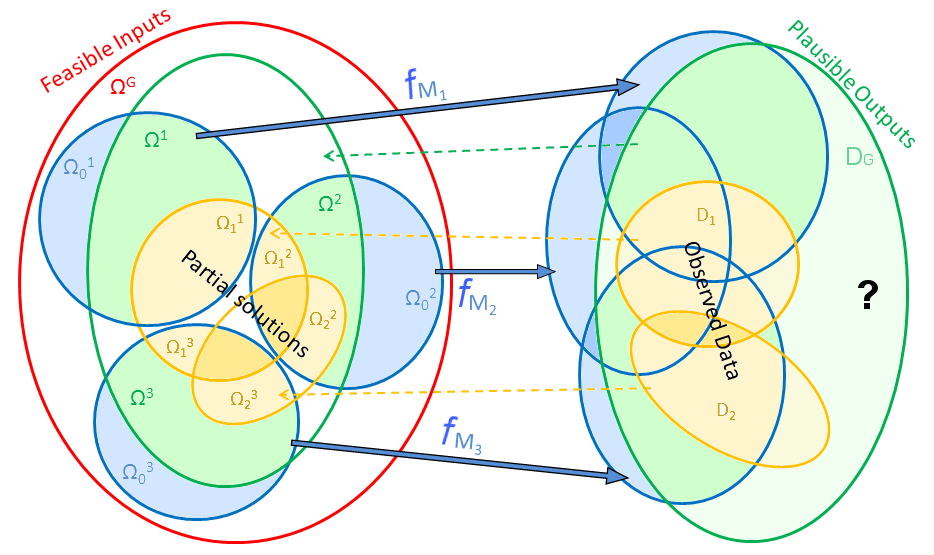
\includegraphics[width=0.85\textwidth]{Scheme_ok3.png}
\caption{Diagram of input spaces, model functions, and output space, with feasible inputs domain (red), plausible output codomain (green), and observed data and partial solutions subsets (yellow).}
\label{scheme}
\end{figure}

\subsection{Geophysical case study}
We apply our procedure to a case study of the Atenquique volcaniclastic debris flow, which occurred on the flanks of Colima volcano in 1955. We adopt and compare the three depth averaged models \emph{Mohr-Coulomb} (MC) \citep{SavageHutter1989}, \emph{Pouliquen-Forterre} (PF) \citep{Pouliquen1999, ForterrePouliquen2002, PouliquenForterre2002} and \emph{Voellmy-Salm} (VS) \citep{Voellmy1955, Salm1990}, based on the Saint-Venant equations. Input spaces are explored by Monte Carlo simulation based on Latin Hypercube sampling \citep{McKay1979,Owen1992b,Stein1987,Ranjan2014,Mingyao2016}. The three models are incorporated in our large scale mass flow simulation framework  TITAN2D \citep{Patra2005,Patra2006,Yu2009,Aghakhani2016,Patra2018}. So far, TITAN2D has been successfully applied to the simulation of different geophysical mass flows with specific characteristics \citep{Sheridan2005, Rupp2006, Norini2008, Charbonnier2009, Procter2010, Sheridan2010, Sulpizio2010, Capra2011}. Several studies involving TITAN2D were also directed towards statistical study of geophysical flows, focusing on uncertainty quantification \citep{Dalbey2008, Dalbey2009, Stefanescu2012b, Stefanescu2012a}, or on the more efficient production of hazard maps \citep{Bayarri2009, Spiller2014, Bayarri2015, Ogburn2016}.

\section{Nevado de Colima volcano and Barranca de Atenquique}\label{s1}
The Colima Volcanic Complex is located in the western portion of the Trans-Mexican Volcanic Belt (small box in Fig. 1). It consists of a N--S volcanic chain formed by C\'antaro, Nevado de Colima, and Colima volcanoes, within the Colima Graben \citep{Luhr1990}. It began forming 1.7 Ma ago with the growth of C\'antaro Volcano (2800 m.a.s.l), and continued with the formation of Nevado de Colima volcano 0.53 Ma ago \citep{Allan1986, Robin1987}. Activity was intermittent during the Pleistocene and Holocene and continues today at Colima volcano, south of  Nevado  \citep{Saucedo2010, Zobin2015, Macorps2018}.

Nevado de Colima (4320 m.a.s.l.) occupies the central part of the volcanic complex, being the most voluminous of the volcanoes (300�-400 km$^3$). It is characterized by three or four horseshoe-shaped craters \citep{Cortes2010}. The youngest crater is 4 km wide and opens to the east with 100 m deep, vertical walls. This structure contains the summit Picacho dome (4300 m). The eastern flank of Nevado exposes a thick sequence of debris flow, fluvial, pyroclastic flow and debris avalanche deposits known as the Atenquique Formation \citep{Mooser1961, Cortes2005, Saucedo2008}, covered by younger deposits. The crater morphology directs a large part of the drainage from the volcano into the Atenquique ravine, located on the ENE flank of the volcano and $\sim$25 km long. Figure 1 shows the ravine and its surrounding topography.

Plot (\ref{Fig1}b) includes elevation isolines from the SRTM DEM of 30-m cell size for UTM Zone 13N \citep{NASA2014}. The drainage begins at an elevation of 4000 m on the eastern flank of Nevado, is occupied by the perennial Atenquique river, and ends at its junction with the perennial Tuxpan River at 1040 m. Between, 4000 and 2000 m in altitude, the ravine has an average slope of 34$^\circ$. At an elevation of 1800 m, the Atenquique ravine is cut off by a 250 m cliff in the vicinity of the junction with the Dos Volcanes dry ravine. Beyond this cliff, the slope of the ravine suddenly decreases from 34$^\circ$ to 18$^\circ$, keeping this gradient to an elevation of 1600 m at 11.5 km from the summit. Between this site and the catchments of the Los Pl\'atanos and Arroyo Seco dry ravines, located at $\sim$21.5 km at an elevation of 1120 m, the ravine gradient varies from 10$^\circ$ to 6$^\circ$. The town of Atenquique is located at an altitude of 1050 m, and 18.5 km (25 km along the ravine path) from the head of the ravine, where the ravine channel has a gradient of 5$^\circ$, which is maintained down to the confluence with the Tuxpan River. Atenquique ravine has an average width of 30 m, although in the vicinity of Atenquique village it is up to 200 m wide.

\subsection{The Atenquique volcaniclastic debris flow, 1955}
On 16/10/1955, at 10:45 am, the inhabitants of Atenquique described the sudden arrival of an 8--9-m high wave carrying mud, boulders and tree trunks that devastated the buildings in the town and four bridges, including the railroad bridge. More than 23 people died, and the flood leveled everything but the tower of the church and the upper part of the market place that luckily served as shelter for survivors \citep{PonceSegura1983, Saucedo2008}. During the peak flow, eyewitnesses observed that complete walls of buildings were displaced several meters by the flood prior to their collapse. The deposits are exposed along the Atenquique, Arroyo Seco, Los Pl\'atanos and Dos Volcanes ravines, and their distribution, stratigraphy, granulometry, and volume have been  described in \cite{Saucedo2008}. Sixty stratigraphic sections were studied along the Atenquique ravine and its main tributaries  (Fig. \ref{Fig1}). Deposits cover a minimal area of 1.2 km$^2$, and with an average thickness of 4 m, a minimum volume of 3.2$\times10^6$ m$^3$ was estimated for the flow.
\begin{figure}[H]
\centering
\includegraphics[width=1\textwidth]{Fig1.jpg}
\caption{Barranca de Atenquique (M{\'e}xico) overview. (a) Stratigraphic sections of \citep{Saucedo2008} are marked with red dots, including 5 preferred locations (stars) and major ravines. Shaded sites are detailed in Supporting Information. Initial source piles are marked by blue dots. Coordinates and projection are UTM zone 13N WGS84. (b) Digital elevation map including isolines \citep{NASA2014}. Volume partition percentages among sources are reported. Regional map is included in a small box.}
\label{Fig1}
\end{figure}
The main flood probably formed in the Atenquique ravine, but was enhanced by the confluence of flows from its tributaries: Dos Volcanes at 11.2 km, Arroyo Seco and Los Pl\'atanos, at 22.5 km. During the first 10 km (as recorded by the proximal exposures) the flow moved down steep slopes, eroding and incorporating coarse alluvium and sand. Downstream, in the medial exposures, the flow encountered gentler slopes, reducing its velocity and promoting deposition of part of the sediment load. Just upstream of the village, below the junction with the Arroyo Seco and Los Pl\'atanos ravines, eyewitnesses reported peak flood levels, possibly enhanced by the engulfing of a small water reservoir. At the junction, the flow captured the fine-material load of flow from the Arroyo Seco and Pl\'atanos ravines, causing significant dilution and a sudden increase in the flow turbulence. Downstream from the town, the flow lost its capacity to transport large boulders, probably due to widening of the reach and the consequent fall in velocity, which was further reduced by the hydraulic roughness effects of the flow impacting buildings. The diluted flow probably had a velocity in the range of 4 to 6 m/s, obtained by comparison with analog flows \citep{Pierson1985, Saucedo2008}. The flood finally continued downstream to join with the perennial Tuxpan River, where it emplaced up to 6 m of deposits.

\subsection{Multiple sources and their locations}
The 1955 debris flow, according to eyewitness accounts and deposit analyses, emanated from multiple sources throughout the watershed. The existence of multiple source areas presents a unique challenge when attempting to model the flow. Eyewitnesses confirm that after the event, many small landslides scars were present along the main ravine and its tributaries. It is hypothesized that these landslides, triggered by rain infiltration, supplied the bulk of the material \citep{Saucedo2003, Saucedo2008}. To account for this, and based on the work in \cite{Rupp2004} we initiate the flow from five major source locations, reported in Fig. \ref{Fig1}. We remark that our numerical simulation toolkit allows for multiple starting points in the same run. Each source consists of a paraboloid pile of material with unitary aspect ratio. Two source locations (\#1 and \#2) are placed in the main ravine, one (\#3) in a lateral valley associated with the regional Tamazula fault, one source (\#4) in Arroyo Seco and one (\#5) in Arroyo Pl\'atanos. These locations are selected based upon local topography. The first three are located on steep upland slopes, while the other two are located along the main drainage due to the lack of steep terrain nearby \citep{Rupp2004}. The partition of volume $V=\sum^5_{k=1} V_k$ among the five sources is scaled based upon the size of the drainage basin they are located within. In particular, $\forall k$ we define $w_k=V_k/V$ as:
$$w_1=w_3=w_4=19.24\%, \quad w_2=37.58\%, \quad w_5=4.70\%.$$
This is equivalent to choosing pile radii of $80\ m$, $100\ m$ and $50\ m$ respectively. We note that, considering the thickness and volume of the related deposits, additional testing could be focused on tentatively increasing the weight of the fifth source. Nevertheless, if compared to the other ravines, Arroyo Seco basin is not characterized by steep topography (\ref{Fig1}). So, a significant volume increase would require a different definition of the source geometry, which is outside the purposes of this study.

We remark that source number, location, and volume partition will be preserved in the following analysis. However, we tested whether small variations affect the character of the simulated flow only proximally. Large variations would require additional field work to be justified, and are beyond the purpose of this study. More details about volume $V$ are provided in Section \ref{sub2.1}.

\section{Probabilistic modeling in a prediction-oriented framework}\label{s2}
Our numerical modeling of the Atenquique flow proceeds by first assuming that the laws of mass and momentum conservation hold for properly defined system boundaries. The flow had very small depth compared to its length, and hence we assume that it is reasonable to integrate through the depth to obtain simpler and more computationally tractable equations \citep{SavageHutter1989}. The depth-averaged Saint-Venant type equations that result are:
\begin{eqnarray}
\label{eq:D_A}
\frac{\partial h}{\partial t} +
\frac{\partial}{\partial x}(h \bar{u}) +
\frac{\partial}{\partial y}(h\bar{v}) &=& 0 \nonumber \\
\frac{\partial}{\partial t} (h\bar{u}) +
\frac{\partial}{\partial x}\left(h\bar{u}^2 + \frac{1}{2}k g_{z}h^2\right) + \frac{\partial}{\partial y}(h\bar{u}\bar{v}) &=& S_{x}\\
\frac{\partial}{\partial t} (h\bar{v}) +
\frac{\partial}{\partial x}(h\bar{u}\bar{v}) +
\frac{\partial}{\partial y}\left(h\bar{v}^2 + \frac{1}{2}k g_{z}h^2\right) &=& S_{y} \nonumber
\end{eqnarray}
Here the Cartesian coordinate system is aligned such that $z$ is normal to the surface; $h$ is the flow depth in the $z$ direction; $h\bar{u}$ and $h\bar{v}$ are respectively the components of momentum in the $x$ and $y$ directions; and $k$ is the coefficient which relates the lateral stress components, $\bar{\sigma}_{xx}$ and $\bar{\sigma}_{yy}$, to the normal stress component, $\bar{\sigma}_{zz}$. Note that $\frac{1}{2} k g_z h^2$ is the contribution of hydrostatic pressure to the momentum fluxes. $S_x$ and $S_y$ are the sum local stresses: their definition depends on the constitutive model of the flowing material \citep{Kelfoun2011}. These include the gravitational driving forces, the basal friction force resisting to the motion of the material, and additional forces specific of rheology assumptions.

In this study we adopt the \emph{Mohr-Coulomb} (MC), \emph{Pouliquen-Forterre} (PF) and \emph{Voellmy-Salm} (VS) models, detailed in Appendix  \ref{A-1}. These three models for large scale mass flows are incorporated in our large scale mass flow simulation framework  TITAN2D \citep{Patra2005}. The $\mathrm{4^{\mathrm{th}}}$ release of TITAN2D \footnote{available from vhub.org} offers multiple rheology options in the same code base. The availability of three distinct models for similar phenomena in the same tool provides us with the ability to directly compare  outputs and internal variables in all the three models and control for usually difficult to quantify effects like numerical solution procedures, input ranges and computer hardware \citep{Patra2018}.

\subsection{Preliminary definition of the input space}\label{sub2.1}
The definition of the input space hierarchy $\mathbb R_+^{d_j}\supseteq\Omega_0^j\supseteq\Omega^j\supseteq\Omega^j_i$, $\forall i,j$, is a fundamental part of our approach. The dimensionality $d_j$ is a characteristic of the model. The input spaces of MC and VS have three dimensions, and are therefore parameterized:
$$\Omega_0^{\mathrm{MC}} = \left\{(\phi_{bed}, \phi_{int}, V)\in \mathbb R_+^3\right\},$$
$$\Omega_0^{\mathrm{VS}} = \left\{\left[\arctan(\mu),\log_{10}(\xi),V\right]\in \mathbb R_+^3\right\}.$$
On the other hand, the input space of model PF originally has six dimensions - $(\phi_1, \phi_2, \phi_3, \beta, L, V)$. Following \cite{PouliquenForterre2002}, we constrain $\phi_3=\phi_1+1^\mathrm{\circ}$. Moreover, preliminary testing in our case study showed a very similar impact from the variation of $\beta$ and $L$. So, we were able to further reduce $d_{\mathrm{PF}}=4$, by assuming the empirical relationship:
\begin{equation}
\beta=f(\phi_2):=\frac{\phi_2 - 7^\circ}{20} + 0.1,
\end{equation}
which is  consistent with the $\beta$ values presented in literature \citep{PouliquenForterre2002, ForterrePouliquen2003}. We thus effectively parameterize:
$$\Omega_0^{\mathrm{PF}} = \left\{(\phi_1, \phi_2, L, V)\in \mathbb R_+^4\right\}.$$

\subsubsection{General input space}
The input space boundaries $\left(a_{k,{M_j}},b_{k,{M_j}}\right)_{1\le k\le d_j}$ of $\Omega_0^j$ are constrained by the general assumptions:
\begin{itemize}
\item \textbf{Total Volume:} $V\in[3.5,\ 5] \times 10^6\ m^3$, i.e. $4.25 \pm 0.75$ $\times 10^6\ m^3$.
\item \textbf{Input space constraints:}
\par\noindent \textbf{MC} - $\phi_{bed} \ge 5^\circ$, $\quad \phi_{int} \in [\phi_{bed},\ 45^\circ]$.

\vskip.1cm\noindent \textbf{PF} - $\phi_1 \ge 1^\circ$, $\quad \phi_2 \in [\phi_1+6^\circ,\ \phi_1+18^\circ]$, $\quad L \in [0.1,\ 0.5]\ m$.

\vskip.1cm\noindent \textbf{VS} - $\arctan(\mu)\ge 1^\circ$, $\quad \log_{10}(\xi)\le 4$.
\end{itemize}
In particular, a minimum volume of $3.2 \times 10^6\ m^3$ for the deposit left by the flow was obtained by \cite{Saucedo2008}. We assume that it is reasonable to increase this volume by about 10\% to 50\% to represent the potential real volume in the simulated flow, given the lack of recovery of any deposit for the portion of the flow reaching the Tuxpan river. We exclude basal friction angles below $5^\circ$ in MC, and $1^\circ$ in PF and VS because of numerical instability and unphysical behavior. In MC, we constrain $\phi_{bed}<\phi_{int}$, and we exclude internal friction angles over $45^\circ$ because these are not considered realistic. In VS we do not allow $\xi$ over $10^4$ because it produces unphysical results. In PF we constrain  $\phi_1+6^\circ<\phi_2<\phi_1 + 18^\circ$, extending the range of values presented in literature \citep{PouliquenForterre2002, ForterrePouliquen2003}. The parameter $L$ is related to the particle size \cite{ForterrePouliquen2003},  hence we define it consistent with the observed average clasts sampled in the field \citep{Saucedo2008}.

\subsubsection{Specialized input space}
The construction of $\Omega_0^j$ relies on extensive testing of the models over the general input space defined above. We base our analysis on two qualitative properties that any realistic  flow must have: (i) the flow must reach the town of Atenquique in a reasonable time, (ii) the flow does not over-top the ravine walls. We quantitatively re-formulate these properties as:
\begin{itemize}
\item[(i)] the flow reaches a minimum elevation $h<1200$ m a.s.l. before $t=1200$ s,
\item[(ii)] the maximum over-spill at the confluence of flows from different sources is $<0.1$ m thick.
\end{itemize}
In (i), we selected $1200$ m elevation because it is located about 1 km upstream from the village \citep{Saucedo2008}, and $t=1200$ s, because we observed that flows that require more time are not able to realistically inundate the village. In (ii) we focused on flow confluences because they are where the major over-spilling issues take place in our tests. Small changes in this definition  not significantly affect the following analysis.
\begin{figure}[H]
\centering
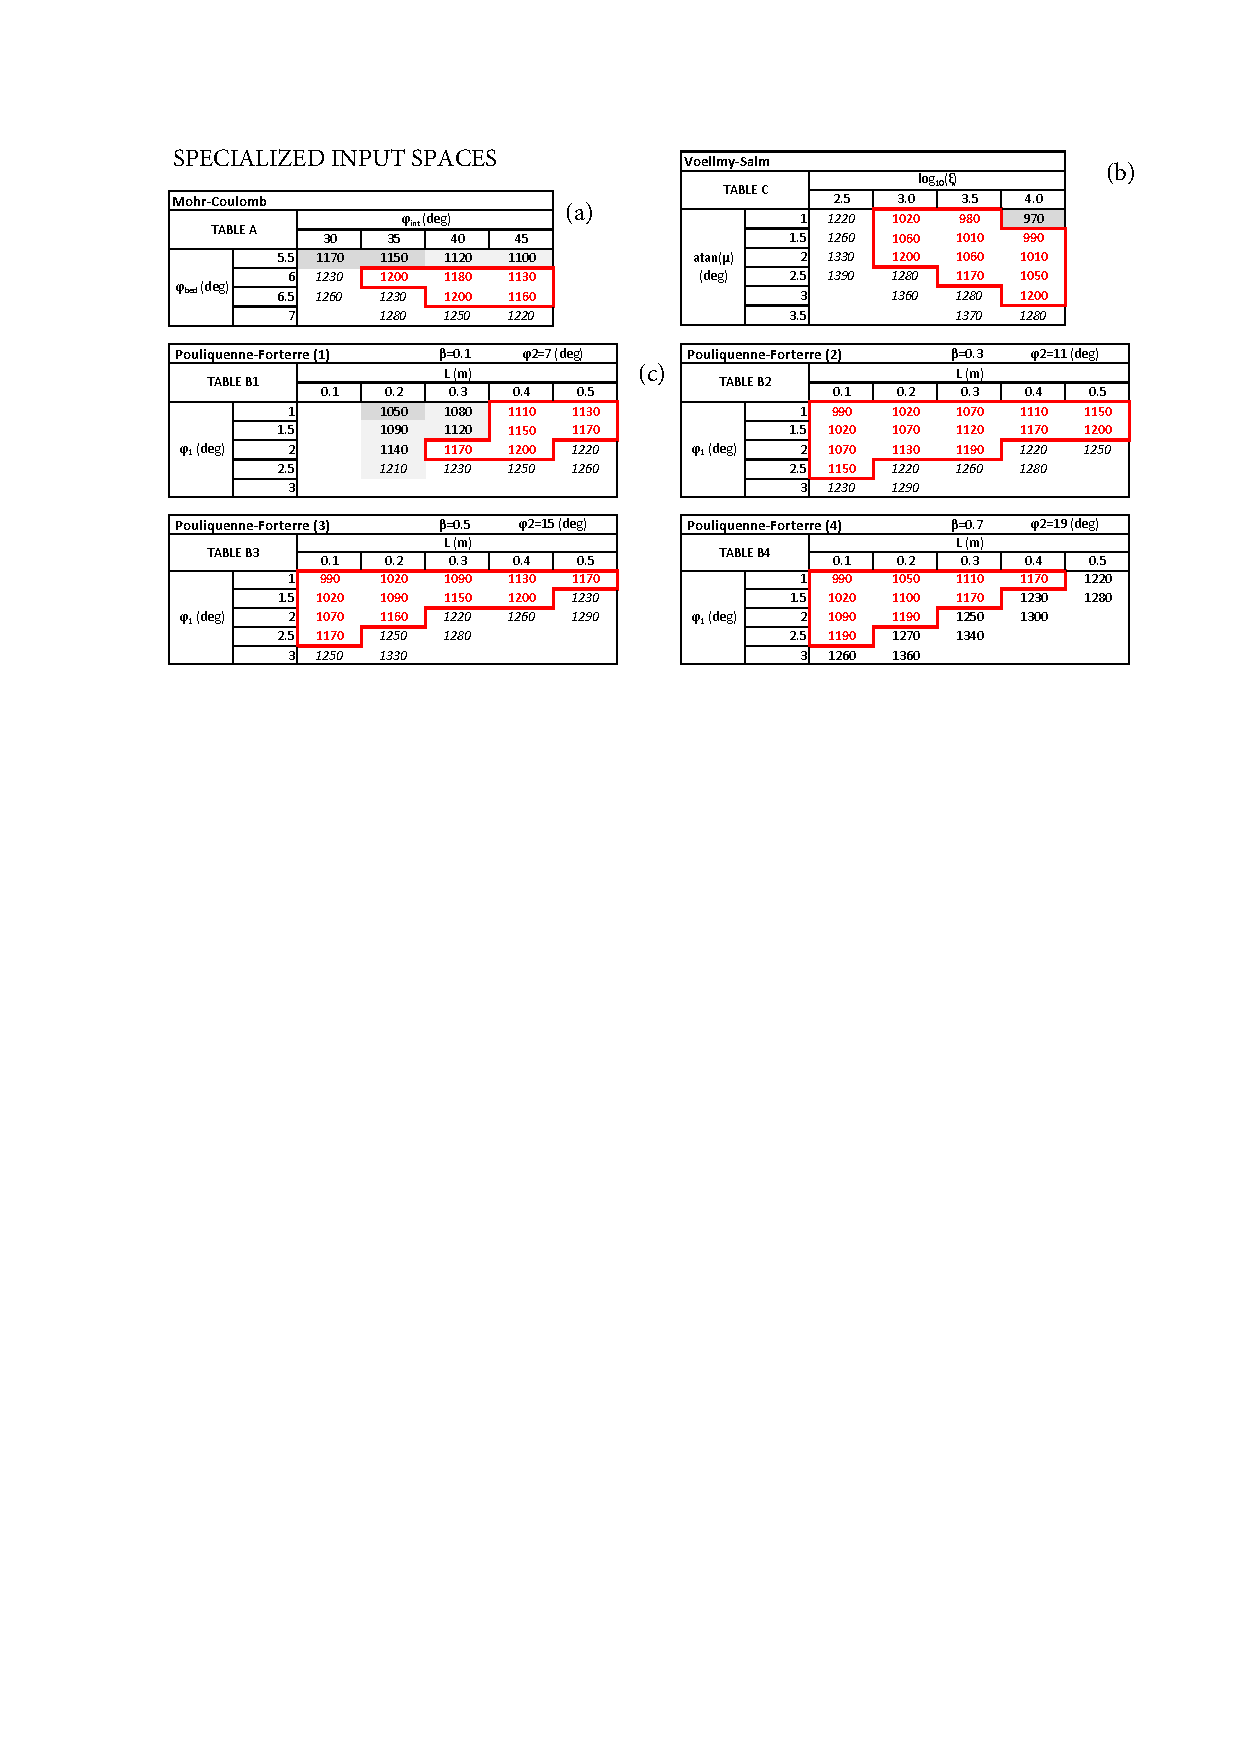
\includegraphics[width=0.95\textwidth]{Table1.pdf}
\caption*{Table 1: Input space explorative testing of (a) MC, (b) VS, (c) PF models, $V=4.18\times 10^6$ $m^3$. The 3D input space of PF is described by four 2D subspaces. Values reported are the minimum elevation $h$ reached at $t=1200$ s. A gray background marks those inputs that generate unphysical flow run-up and over-spill the ravine walls, light gray if $>0.1$ m, dark gray if $>1$ m. Red lines mark the subdomain $\Omega^j$ of flows with $h\le1200$ m and without significant over-spill issues.}
\end{figure}
Table 1 reports the minimum elevation inundated at $1200$ s, and a summary of over-spill issues. These values are generated with reference to a flow volume of $V=4.18\times 10^6$ $m^3$, roughly equivalent to the mean value of our range, and so the input spaces have two dimensions in MC and VS, and three in PF. Following the empirical falsification principle, we snip the input range by  deleting those regions that do not satisfy our requirements. The  subspaces obtained by this procedure do not have rectangular shape, but look like parallelograms - this is because the effects of the input variables on the output are not independent. Maximum flow height maps of all these tests are included in Supporting Information SI1-SI3.

\begin{itemize}
\item In MC we observe over-spill issues if $\phi_{bed} < 6^\circ$, and a  runout that is too short if $\phi_{bed} > 6.5^\circ$. We also note an increase in the runout distance as $\phi_{int}$ increases. In particular, $\phi_{int} \ge 35^\circ$ is required to inundate the village.
\item In VS the over-spill is observed in the region $\{\arctan(\mu)<1.5^\circ\} \times \{\log_{10}(\xi)>3.5\}$. In contrast, the region $\{\arctan(\mu)>3^\circ\} \times \{\log_{10}(\xi)<3\}$ produces runouts that are too short.
\item Model PF must be treated with greater care because of its higher dimensionality. We divide its behavior along four different hyperplanes, corresponding to different values of $\phi_2$ and $\beta=f(\phi_2)$. Over-spill was observed only in the hyperslice with $\phi_2=7^\circ$, and $L<0.4$ m. In general, $\phi_1<3^\circ$ is required to have a long-enough runout.
\end{itemize}

\subsection{Probability measures and specialized experimental design}
Initially, $\forall j$ we uniformly distribute the measure $P_0^j$ supported in the general input space $(\Omega_0^j, \mathcal F^j_0)$:
\begin{equation}
P_0^j\left(p^j_1,\dots,p^j_{d_j}\right)\sim \bigotimes_{k=1}^{d_j} Unif(a_{k,{M_j}},b_{k,{M_j}}),
\end{equation}
where $(p^j_1,\dots,p^j_{d_j})$ is the parametrization of model $M_j\in\mathcal M$ described above, and $\forall k$, $\left(a_{k,{M_j}},b_{k,{M_j}}\right)$ is the input range. Latin Hypercube Sampling is performed over $[0,1]^{d_j}$.

We enhance the sampling procedure by relying on orthogonal arrays \citep{Owen1992a,Tang1993, Patra2018}. Those dimensionless samples are thus linearly  mapped over the required intervals, providing the general experimental design. Then, according to the definition of the specialized input space, we remove the design points which lie outside of the boundary. The new design is distributed according to the probability measure $P^j$:
\begin{equation}
P^j=P^j_0(\Omega^j)\cdot \iota^j_*(P^j_0)
\end{equation}
push-forward of the inclusion $\iota^j$ of $\Omega^j$ in $\Omega_0^j$, normalized to be a probability. $P^j$ is naturally defined over the $\sigma$-field $\mathcal F^j:=(\iota^j)^{-1}\mathcal F_0^j$.

Figure \ref{Fig2} displays the plot of this specialized experimental design. In PF, the design is immersed in $\mathbb R^4$, and in Figure \ref{FigA1} we show the plot of ancillary experimental designs supported over the four hyperplanes described in Table 1, corresponding to different values of $\phi_2$ and $\beta=f(\phi_2)$.

In the following, our time domain is $T=[0,2400\ s]$, which provides sufficient time for simulated flows to realistically inundate the village, considering the inputs in $\Omega^j$. We call $t_f=2400$ s, the ending time of the simulation.

\section{Observable outputs and contributing variables}\label{s3}
We devise multiple statistical measures for analyzing the data according to the specialized LHS design described in the previous section. In general, we sample the model inputs in a Monte Carlo simulation, and the output of each sample run is calculated as a function $f(\underline{\textbf x},t)$, where $t$ is the time and $\underline{\textbf x}$ is a spatial element of the computational grid. The family of these functions naturally defines a random variable which expresses the model outputs with respect to the probability distribution $P^j$ over the input space $(\Omega^j, \mathcal F^j)$. This analysis generates a tremendous volume of data that we analyze using statistical methods. The results are summarized by a family of spatial maps and temporal graphs, displaying the expectation of the model outputs and also their 5$^{\mathrm{th}}$ and 95$^{\mathrm{th}}$ percentiles, with respect to $P^j$.

In particular, we select five sites and we gather detailed results from our simulations in those special locations. These are called Sites \#1-\#5  (stars in Figure 1). They all belong to the set of the sixty sections studied in \cite{Saucedo2008}, and the corresponding section numbers are also reported. In detail they are:
\begin{itemize}
\item\textbf{Site \#1}, section 23, UTM 656690.1N, 2160985.4E. Along the main ravine $\sim$6 km upstream from the Atenquique village.
\item\textbf{Site \#2}, section 28, UTM 660380.8N, 2162530.8E. In Arroyo Seco tributary $\sim$2.5 km upstream from the confluence.
\end{itemize} 

\begin{figure}[H]
\centering
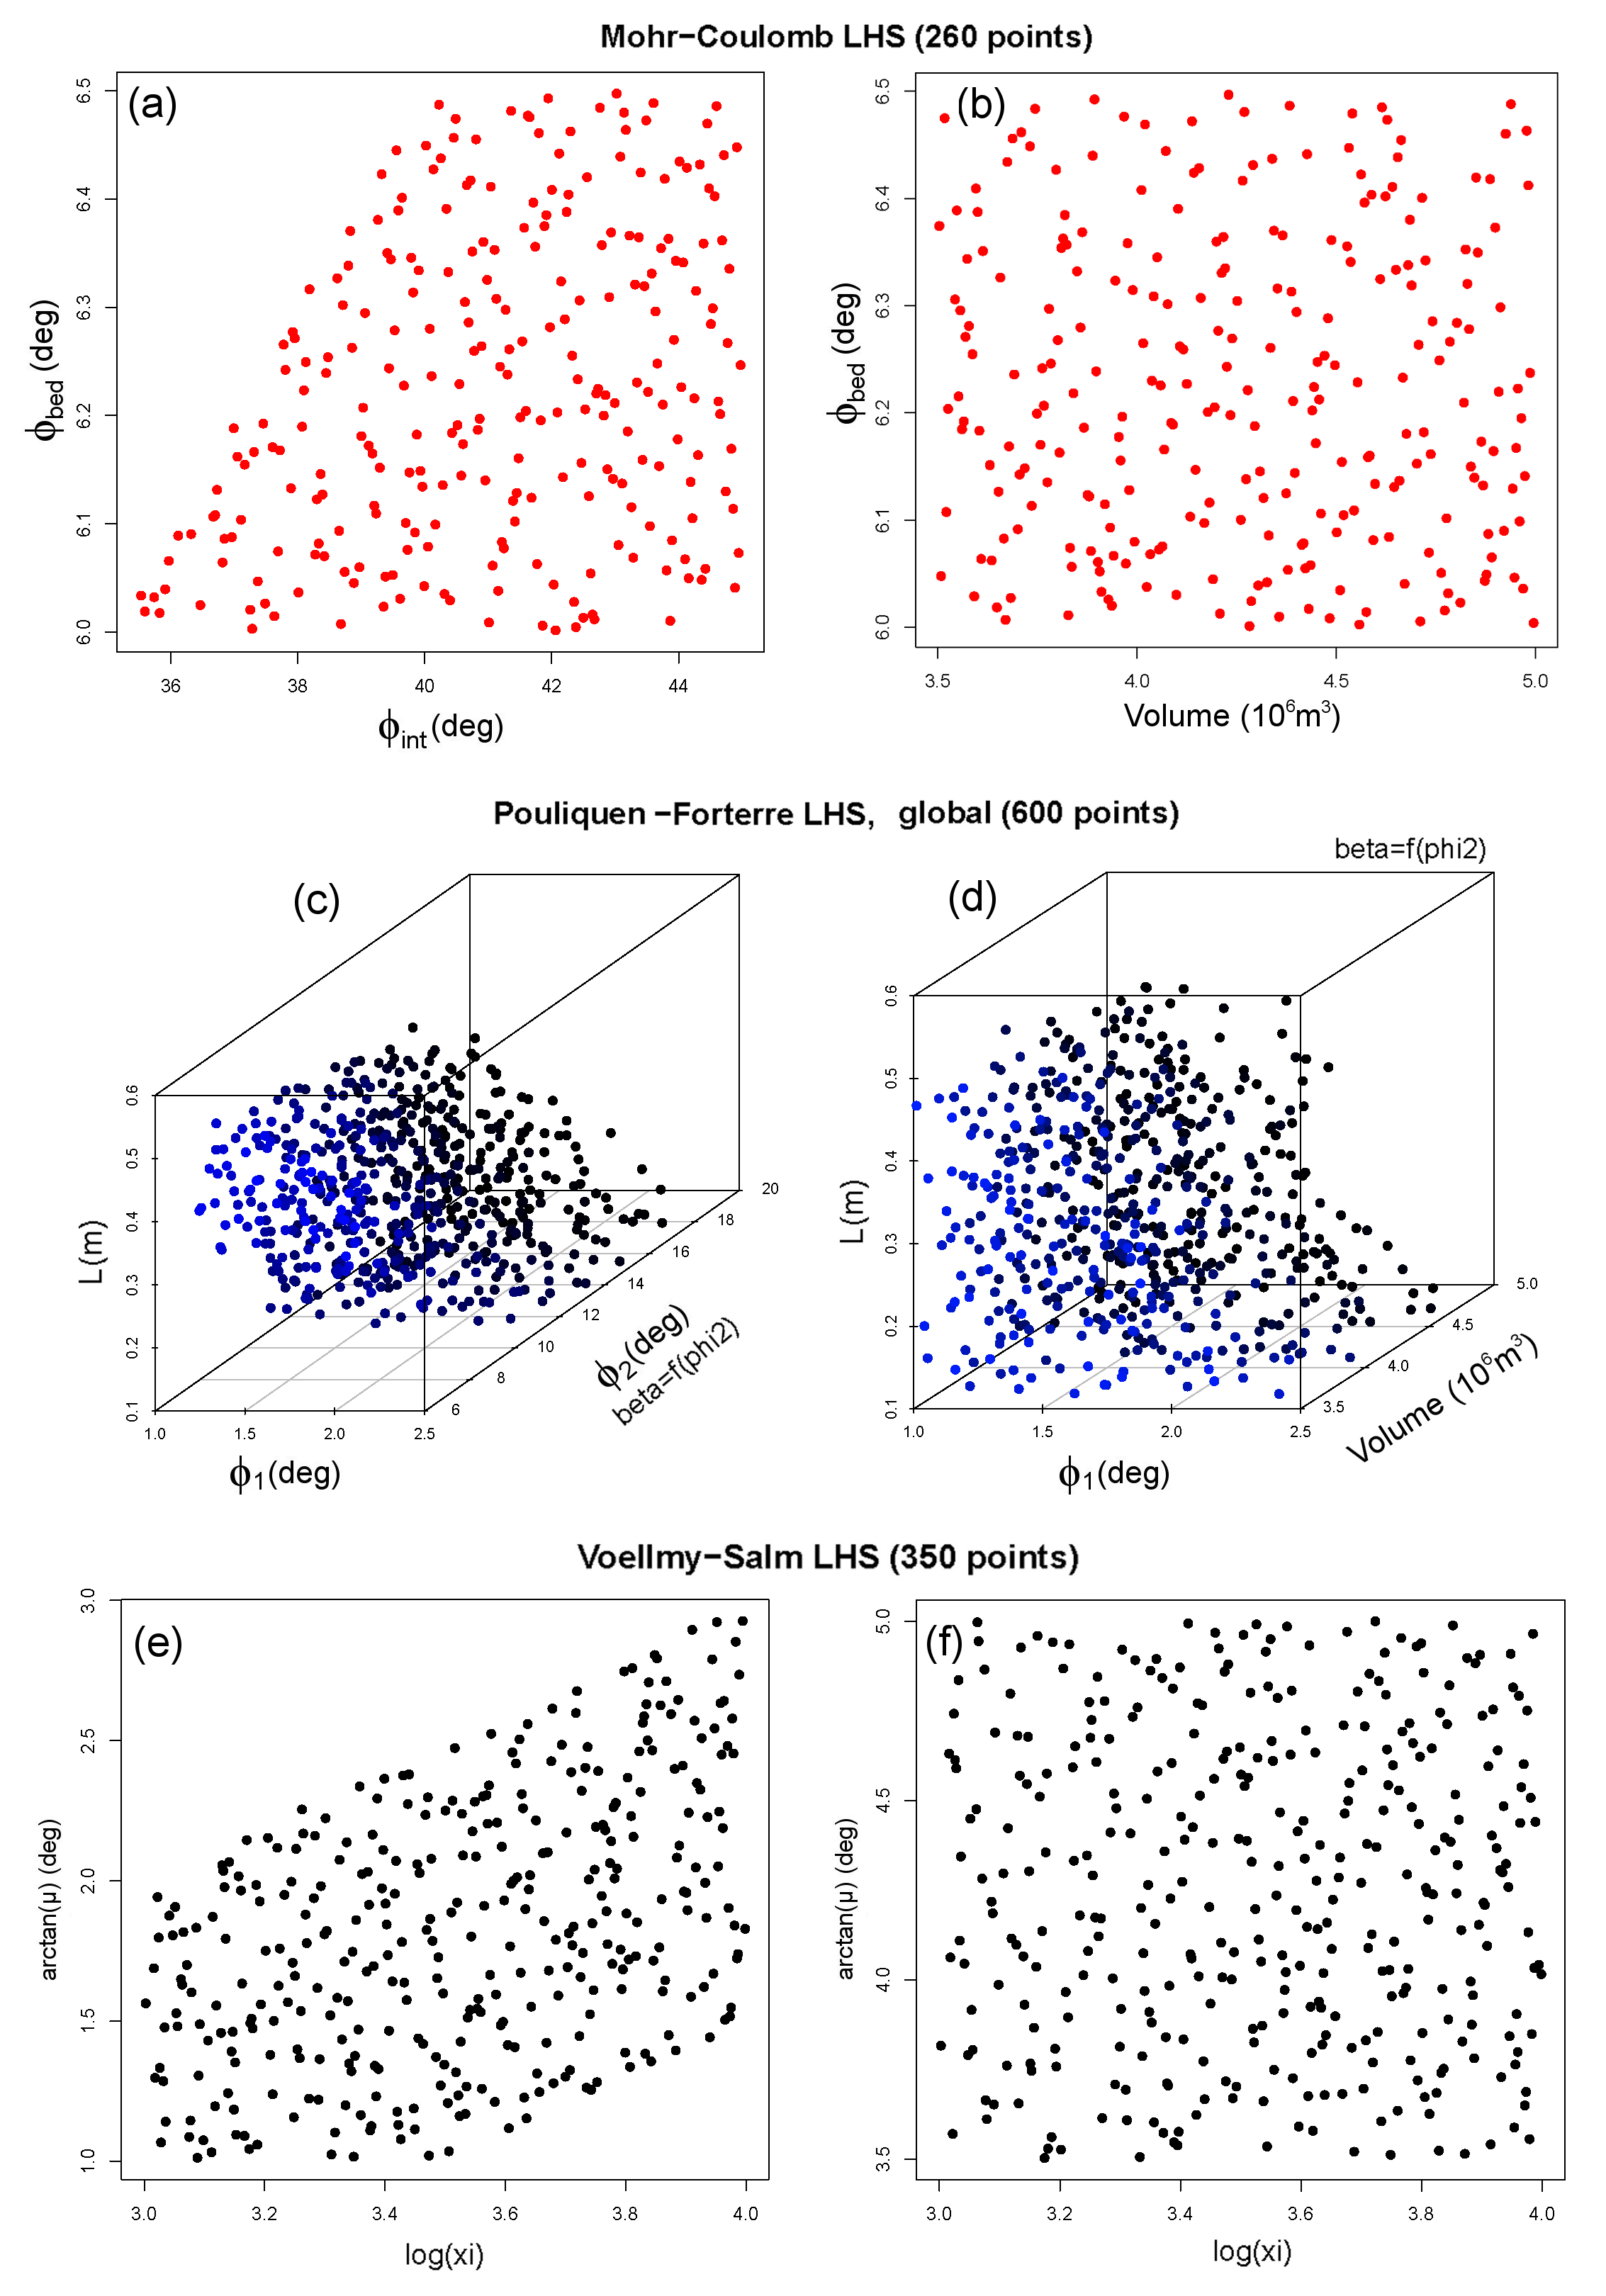
\includegraphics[width=0.87\textwidth]{Fig2.png}
\caption{Overview of the specialized experimental design in (a-b) MC, (c-d) PF, (e-f) VS models. (a-c-e) are projected along the $V$ coordinate, and (b-d-f) along $\phi_{int}$, $\phi_2$ and $\xi$ coordinates, respectively. In (c-d), the color expresses the distance along the third dimension.}
\label{Fig2}
\end{figure}

\begin{figure}[H]
\centering
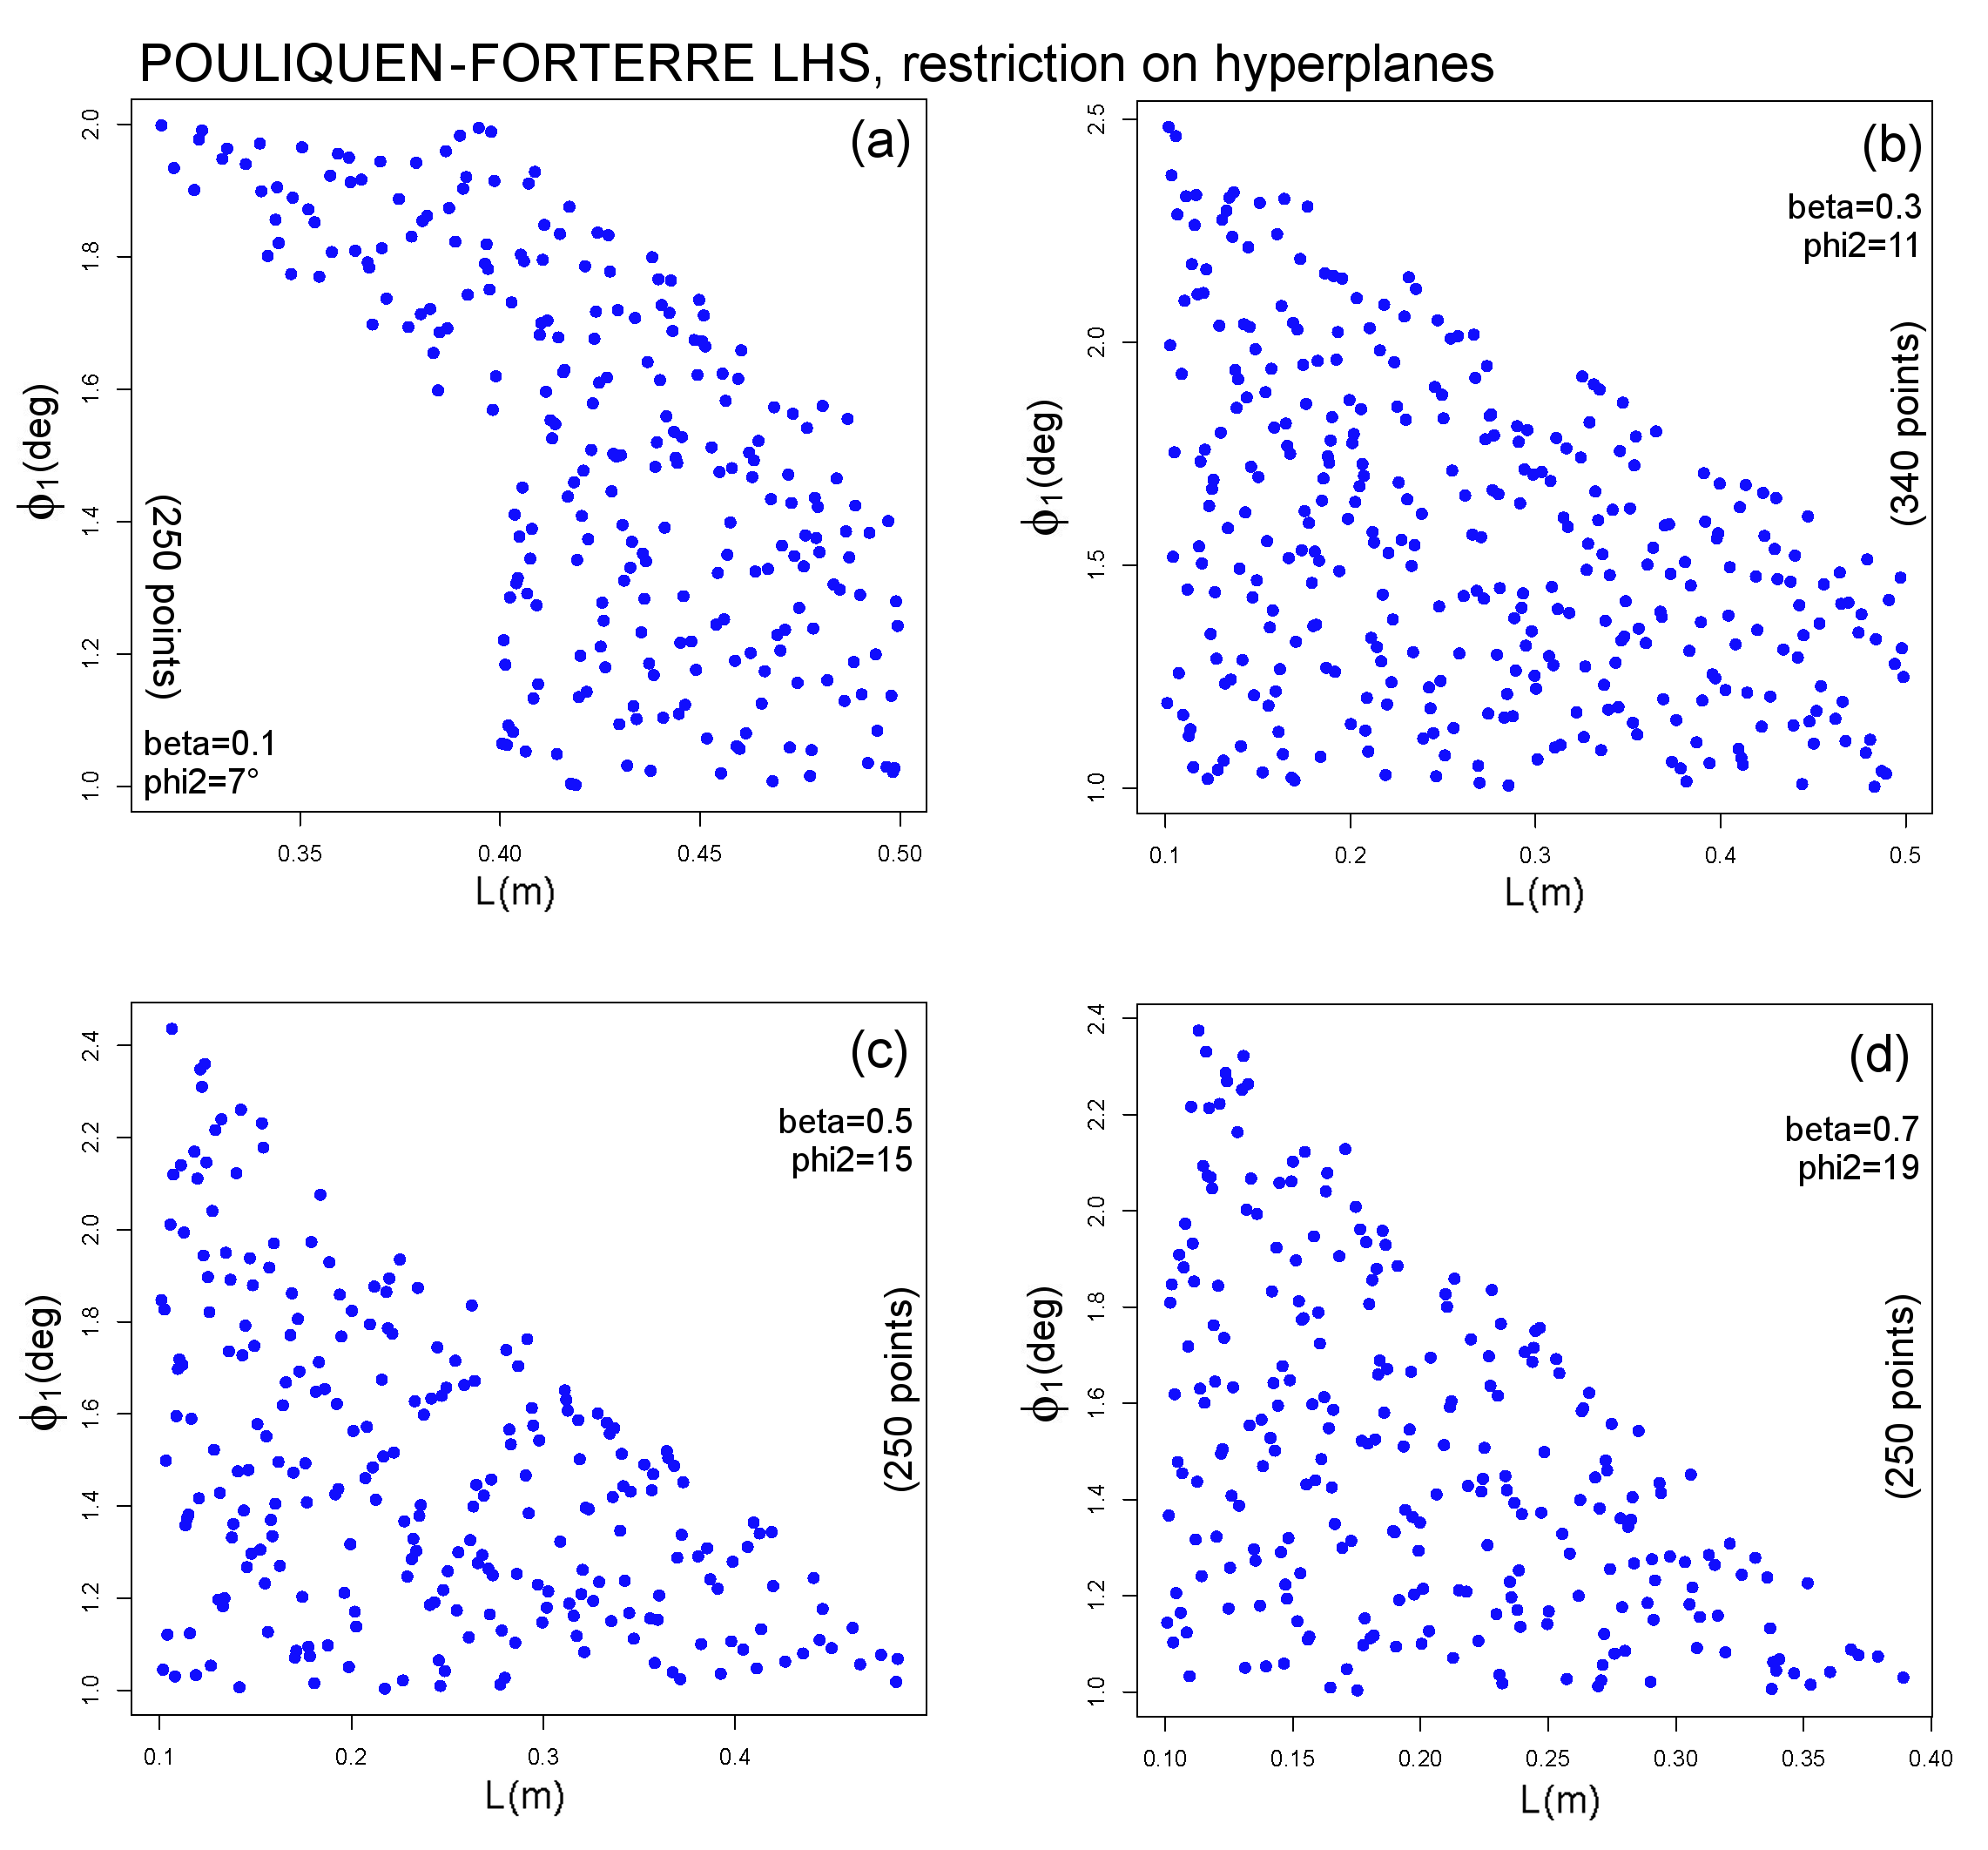
\includegraphics[width=0.85\textwidth]{FigA1.png}
\caption{Overview of modified specialized experimental designs in PF, supported over the four different hyperplanes described in Table 1. All plots are projected along the $V$ coordinate.}
\label{FigA1}
\end{figure}

These first two are not described in detail, but the related results are included in Supporting Information SI4-SI5. Conversely, we focus our analysis on the other three points, all placed along the main ravine in proximity to Atenquique village.
\begin{itemize}
\item\textbf{Site \#3}, section 21, UTM 660258.1N, 2161315.2E. It is $\sim$2 km upstream from the village;
\item\textbf{Site \#4}, section 17, UTM 662453.1N, 2160360.1E. Immediately upstream from the village, close to the confluence with Arroyo Seco and Arroyo Pl\'atanos tributaries;
\item\textbf{Site \#5}, section 42, UTM 663539.0N, 2160200.0E. In the village, $\sim$1 km downstream from the previous site.
\end{itemize}
We note that close to Site \#4 there are the supports of the new bridge of the freeway to the city of Colima.

\subsection{Percentile maps of maximum flow depth and kinetic energy}
First of all, we report the spatial maps of maximum flow depth, $h$, and  kinetic energy ,$\kappa$:
\begin{equation}
H:=\max_{t\in T} h(x,y), \quad K:=\max_{t\in T} \kappa(x,y).
\end{equation}

In our depth-averaged approach the \emph{kinetic energy} is defined as:
\begin{equation}
\kappa:=\frac{1}{2} \frac{(h\bar{u})^2+(h\bar{v})^2}{h},
\end{equation}
where $h\bar{u}$ and $h\bar{v}$ are, respectively, the components of momentum in the $x$ and $y$ directions. 
\begin{figure}[H]
\centering
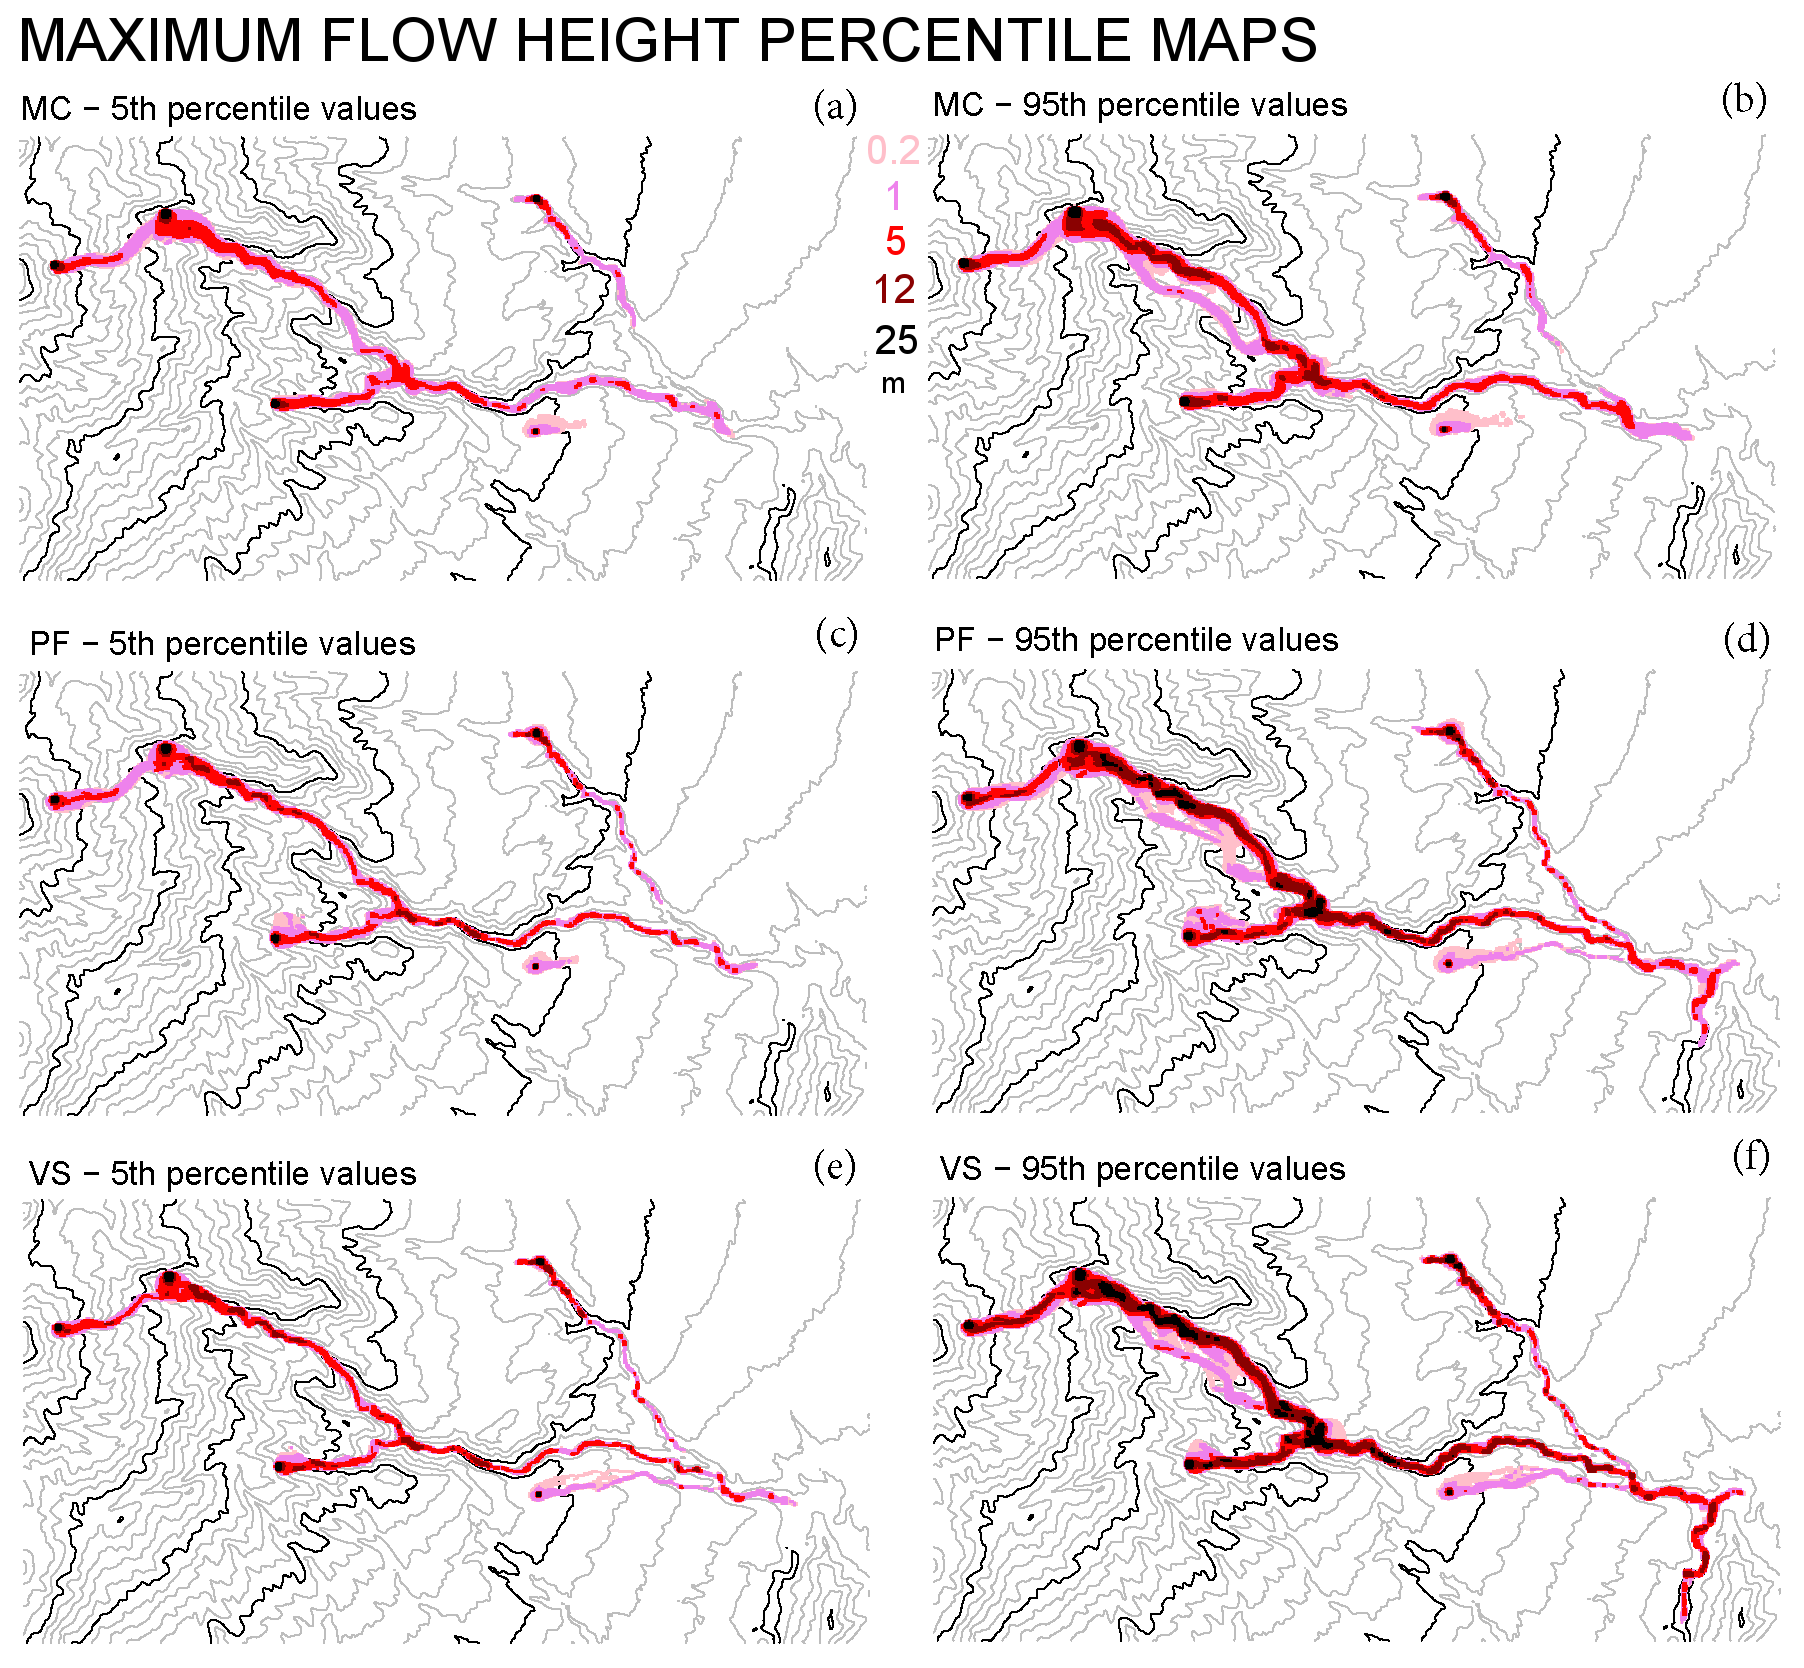
\includegraphics[width=1\textwidth]{Fig3.png}
\caption{Maximum flow height $H$ as a function of time in (a-b) MC, (c-d) PF, (e-f) VS model. (a-c-e) are the 5$^{th}$ and (b-d-f) are the 95$^{th}$ percentile values with respect to $P^j$. Colors are related to the flow height. Elevation contours are included at intervals of 100 m (gray) and 500 m (black) \citep{NASA2014}. Sites \#3,\#4,\#5 are displayed.}
\label{Fig3}
\end{figure}
This is equivalent to $\frac{1}{2} h ||(\bar{u},\bar{v})||^2$, that is half the flow height times the speed square. Thus $\kappa$ is formally the kinetic energy density per unit of surface area,  for a mass with unit density. The kinetic energy, $K$, in a traditional sense may be calculated over an arbitrary region $A$ as:
$$\textrm{Kin}(A)=\rho\int_A \kappa(x,y) dx dy=\rho\int_A \frac{1}{2} h(x,y)\left[\bar{u}(x,y)^2+\bar{v}(x,y)^2\right] dx dy,$$
where $\rho$ is the density of the flow, typically in $[1000,\ 2000]\ kg/m^3$, depending on the flow water content.

Figure \ref{Fig3} reports the maximum flow depth, $H$, and Figure \ref{Fig4} the maximum kinetic energy, $K$. MC shows the lowest values of both flow depth and energy, while VS the highest, especially in the distal part of the domain. In MC, the flow in the tributaries is not capable of reaching the village, while in the 95$^{th}$ percentile maps of PF and VS, it is. In VS, the flow in Arroyo Pl\'atanos joins the main ravine even in the 5$^{th}$ percentile map. In general, local maxima of flow depth are located in the ravine, while the kinetic energy shows a more regular decrease. The energy values at the head of the flow are in $[1,\ 10]\  m^3/s^2$, meaning a relatively slow flow compared to the dynamics observed upstream. Significant over-spill issues are absent, but in the 95$^{th}$ percentile maps all the models report some flow in the Dos Volcanes ravine, of about $[1,\ 5]\ m$ maximum height, and slightly less in PF.
\begin{figure}[H]
\centering
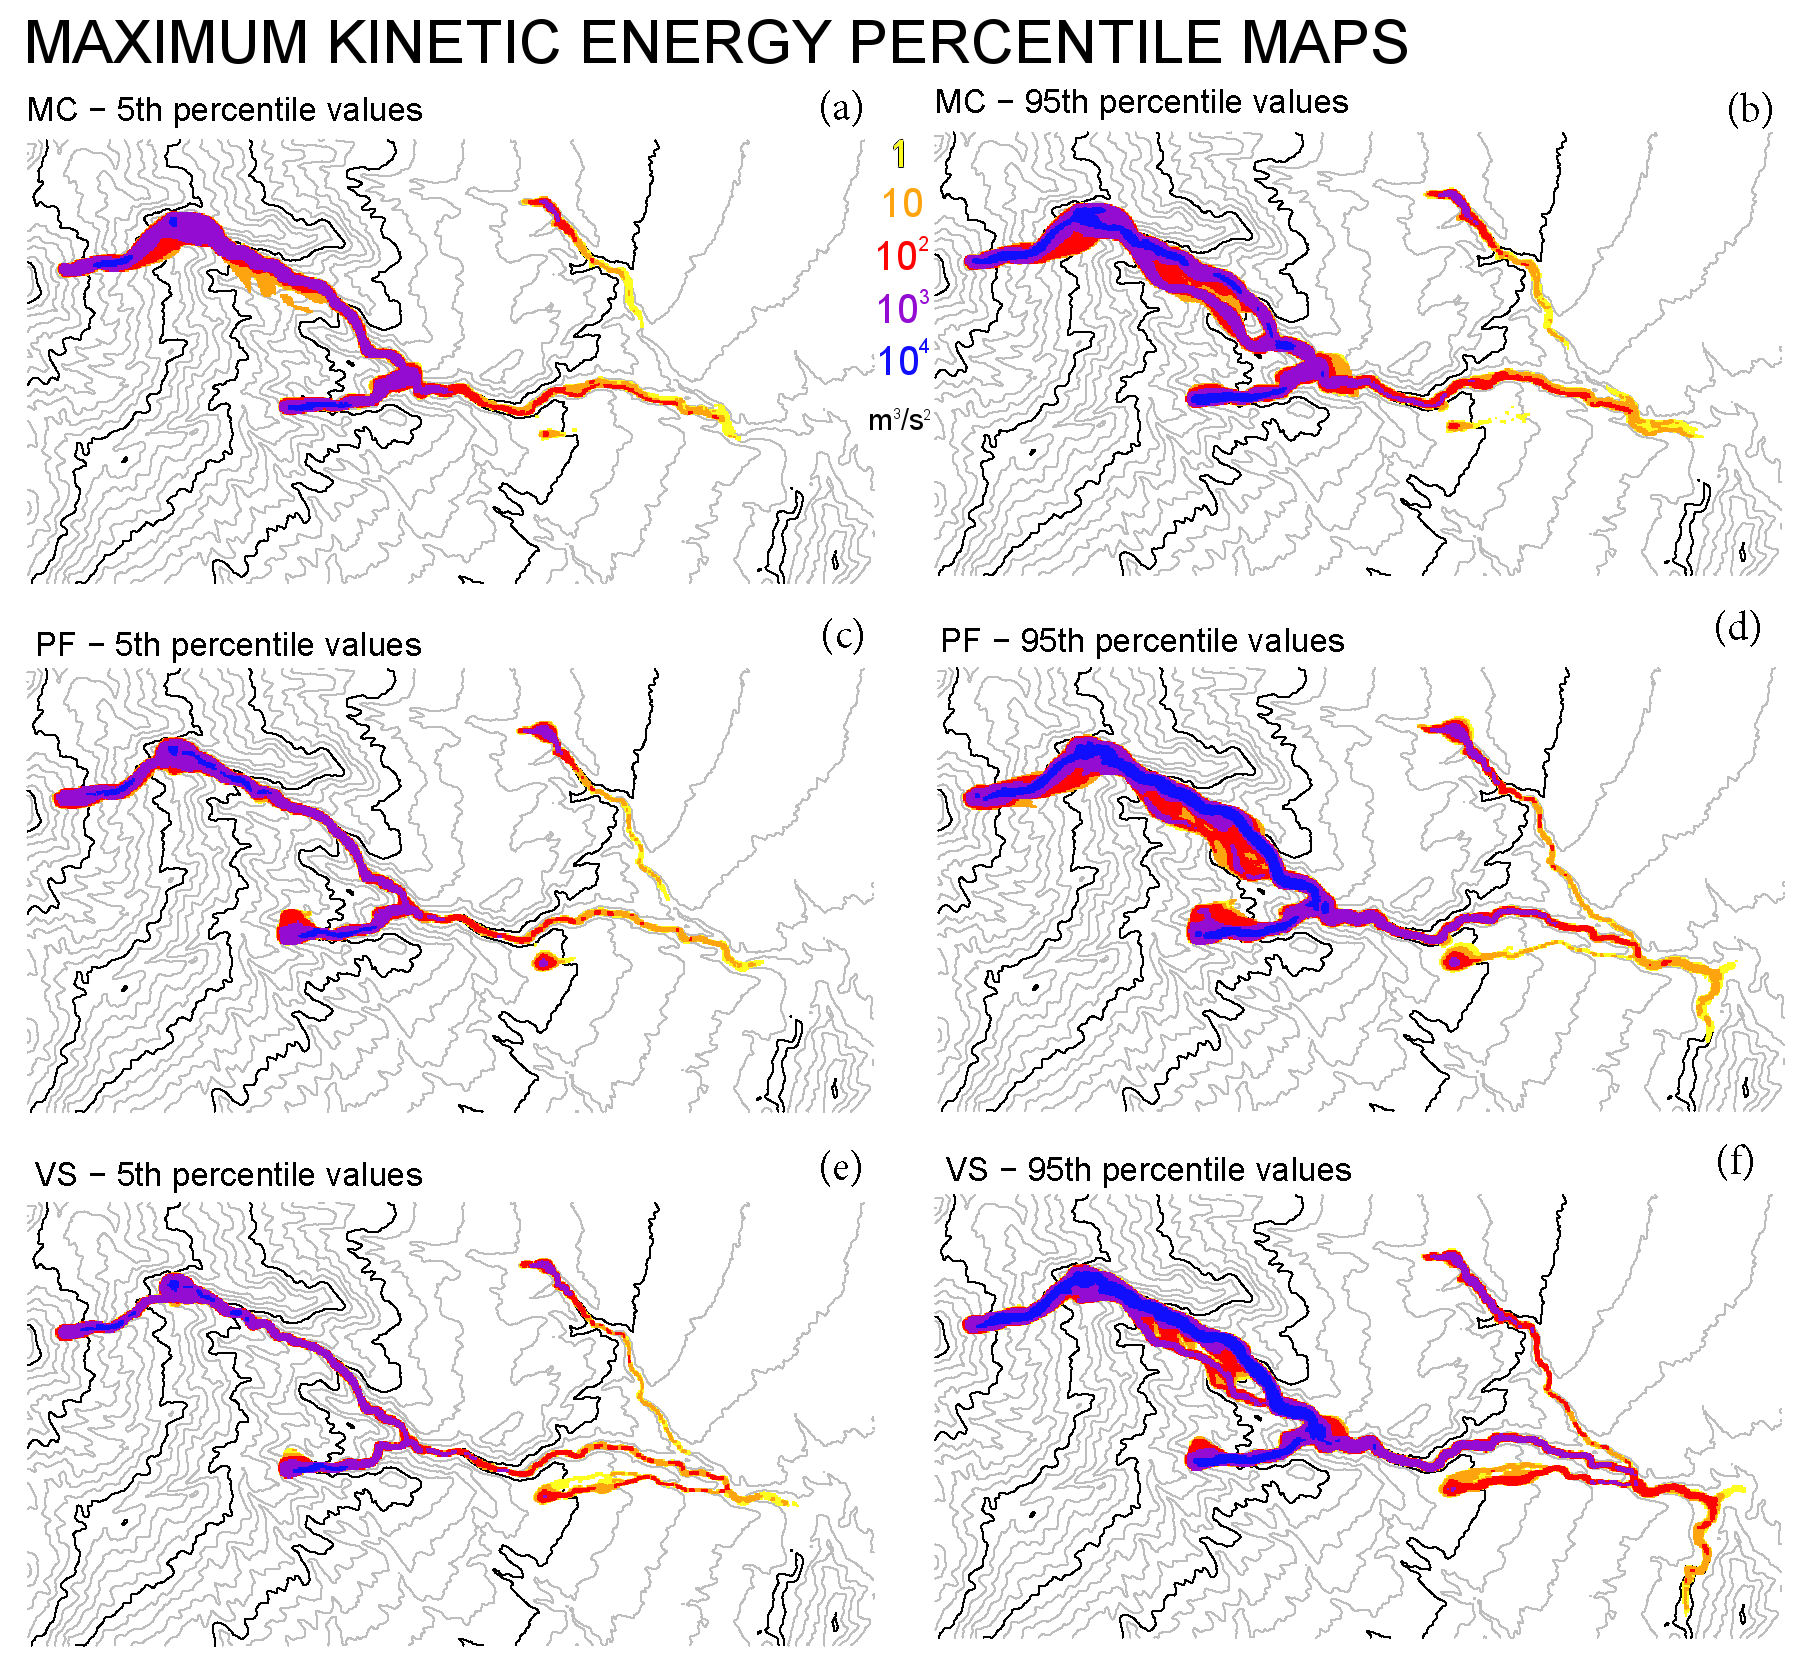
\includegraphics[width=1\textwidth]{Fig4.png}
\caption{Maximum kinetic energy $K$ as a function of time in (a-b) MC, (c-d) PF, (e-f) VS model. (a-c-e) are the 5$^{th}$ and (b-d-f) are the 95$^{th}$ percentile values with respect to $P^j$. Colors are related to the energy in logarithmic scale. Elevation contours are included at intervals of 100 m (gray) and 500 m (black) \citep{NASA2014}. Sites \#3,\#4,\#5 are displayed.}
\label{Fig4}
\end{figure}

\subsection{Local properties of the flow}
We further analyze the flow properties at the three sites selected above, and located in the distal part of the flow (Sites \#3,\#4, \#5), with very different results. All the quantities reported are estimated on the element of the grid which contains the coordinates of the site. We remark that the grid is adaptive, and hence the values can be affected by the size and position of the element. However, the integration over the input space significantly reduces this effect \citep{Patra2018}.

Along with the locally analyzed flow height and speed, we calculate the local \emph{contributing variables} in the modeling equations, that is, the \emph{dominance factors} and the \emph{expected contributions} related to the force terms in the conservation laws that characterize the models. In particular, $\forall n=1,\dots,N$ the dominance factor, $p_n$, is the probability that the force term, $F_n$, is largest. The no-flow probability, $p_0$, is also included, and $\sum_{n=0}^N p_n = 1$. In contrast, $\forall n$ the expected contribution $E^{P_j}\left[C_n\right]$ is the mean of the force term, $F_n$, divided by the greatest (dominant) term. It belongs to $[0,1]$ and represents the degree of relevance of the $n^{th}$ term with respect to the dominant one. Contributing variables and their statistics are introduced in \cite{Patra2018} and detailed in Appendix \ref{A-2}.

The higher dimensionality of $\Omega^{\textrm{PF}}$ requires additional testing. In particular, flow height and speed are  estimated on the hyperplane $\beta=0.5,$ $\phi_2=15^\circ$, and the probability distributions are not remarkably different. Additional plots concerning sites \#1 and \#2 are included in SI4-SI5.
\begin{figure}[H]
\centering
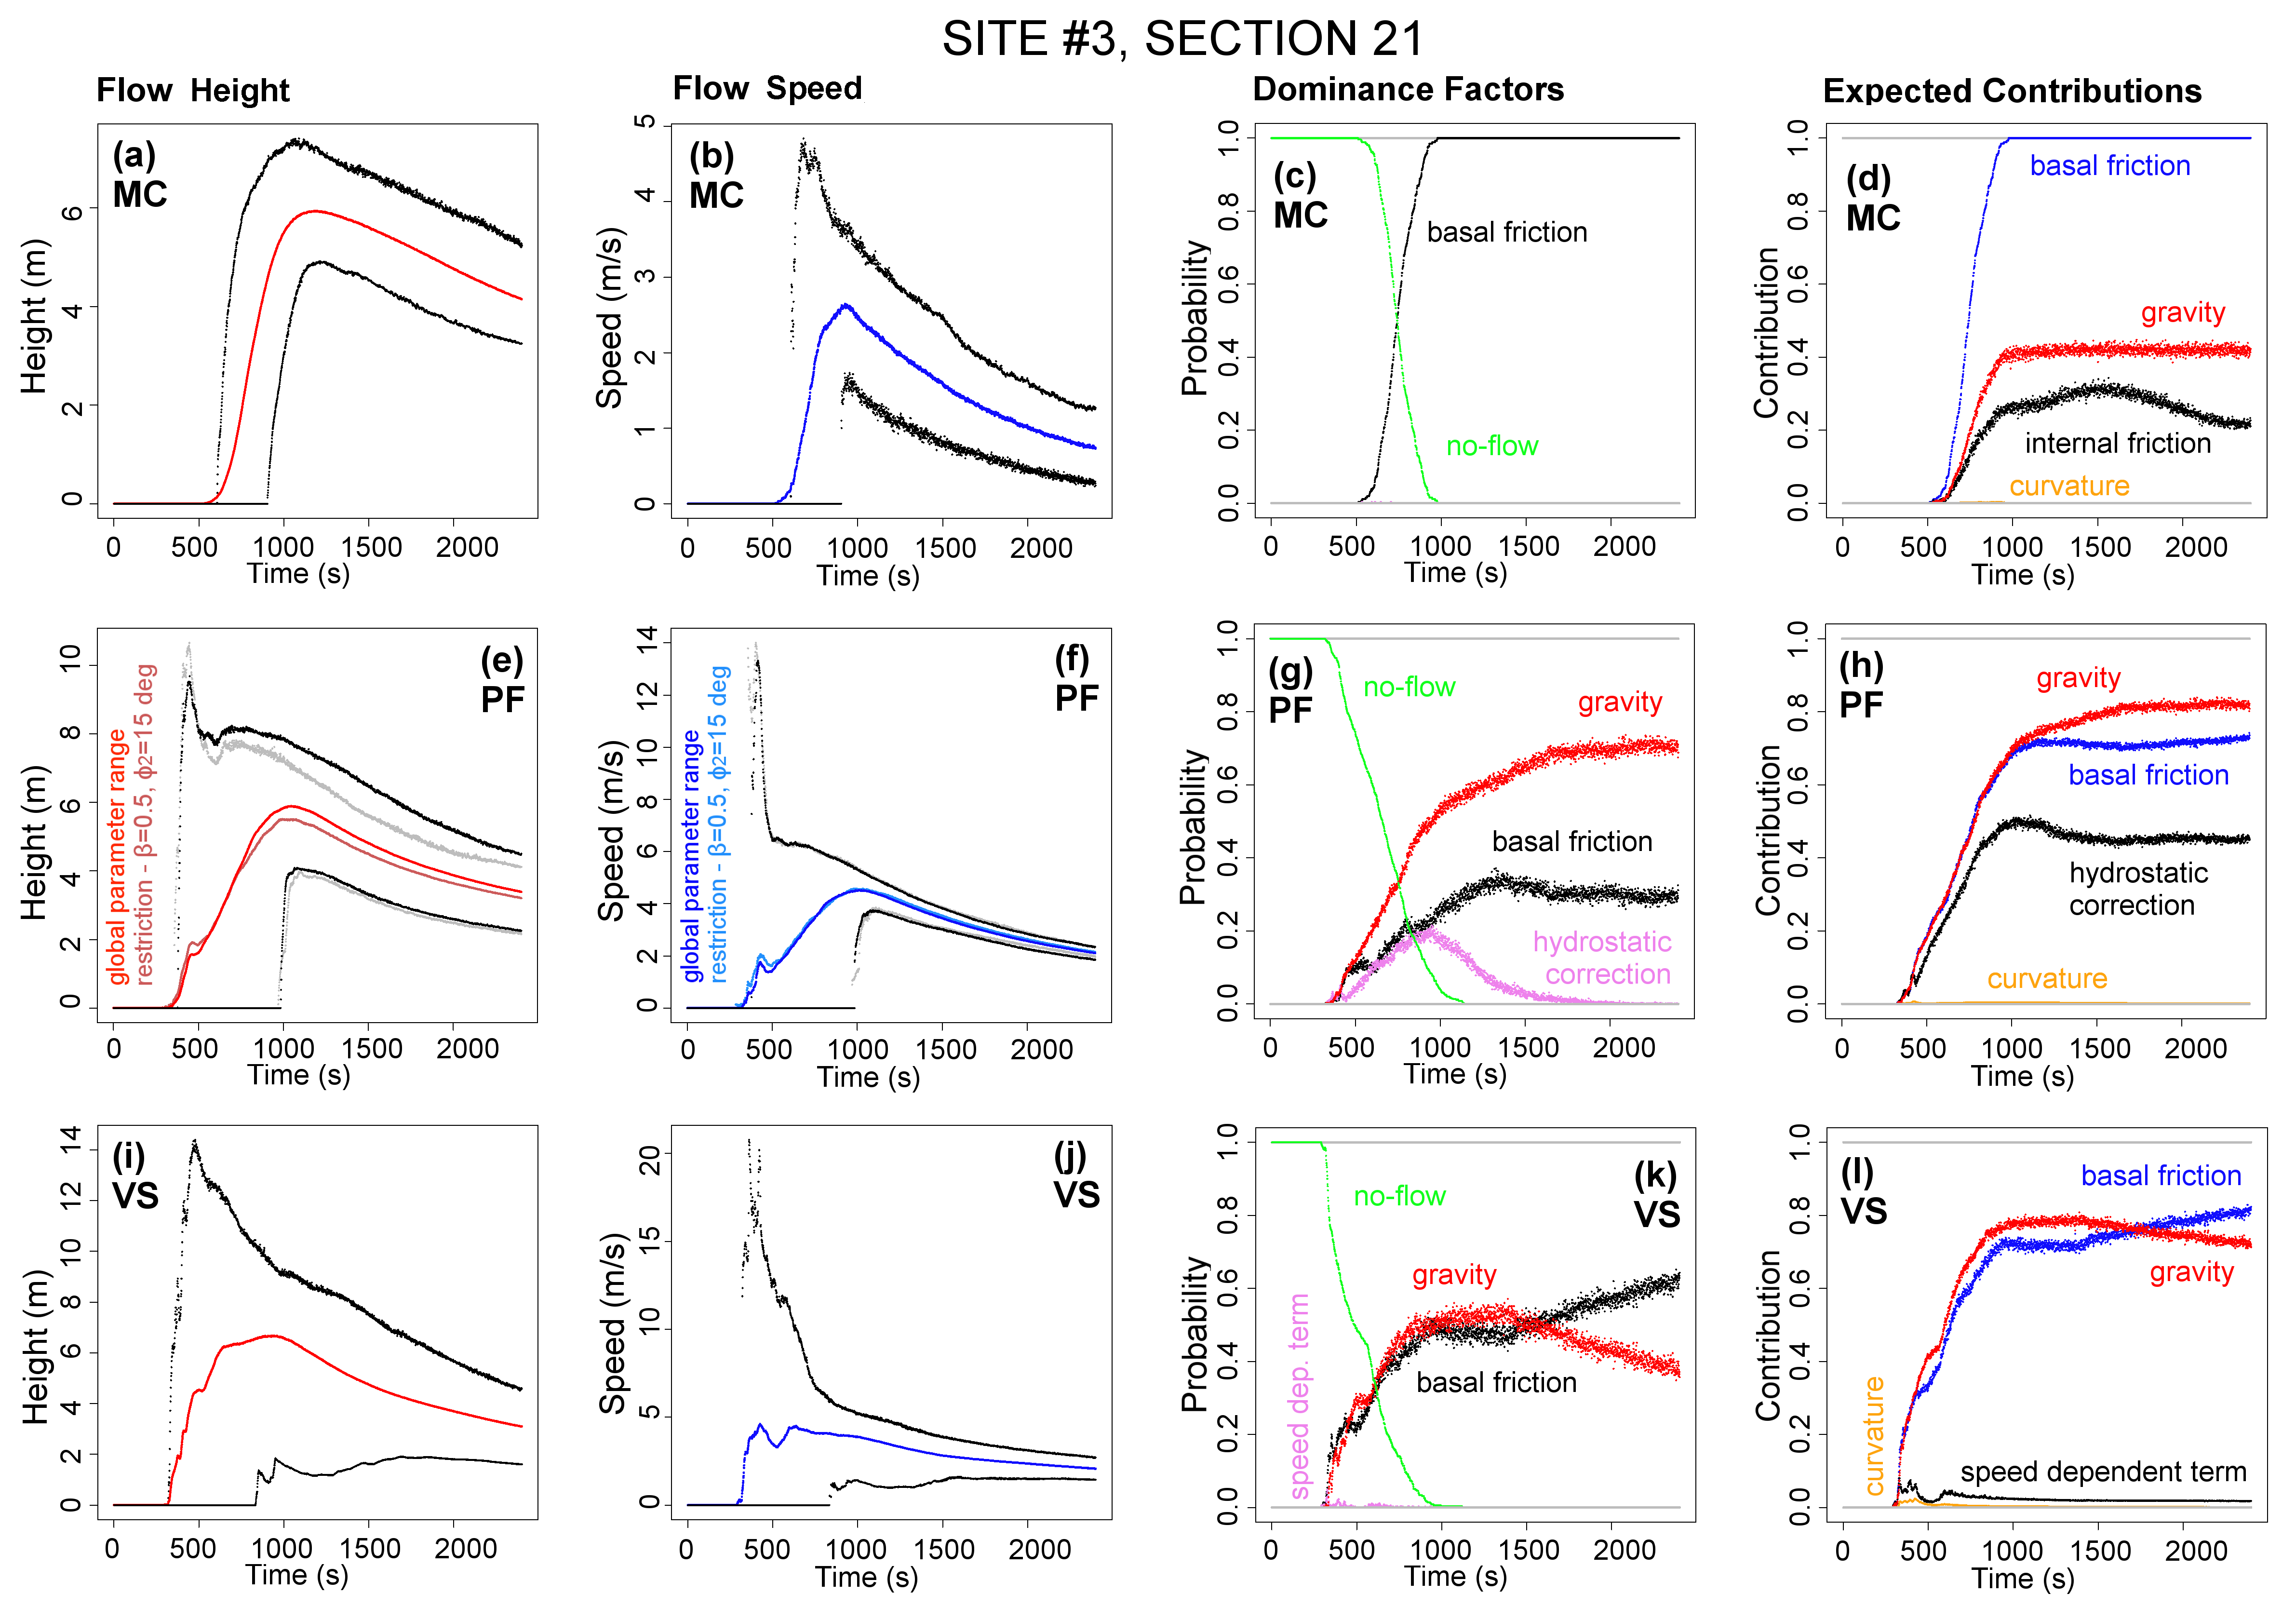
\includegraphics[width=0.97\textwidth]{Fig5.png}
\caption{Local flow properties in Site \#3, $\sim$2 km upstream from Atenquique village. (a,e,i) show flow height, (b,f,j) flow speed, (c,g,k) dominance factors, (d,h,l) expected contributions of the force terms. Different models are plotted separately: (a-d) assume MC; (e-h) assume PF, and (e,f) include estimates on a hyperplanar restriction of the input domain; (i-l) assume VS. In (a,b,e,f,i,j) colored line is mean value, black/gray lines are 5$^{\mathrm{th}}$ and 95$^{\mathrm{th}}$ percentile bounds.}
\label{Fig5}
\end{figure}
Figure \ref{Fig5} shows the local properties at site \#3, located $\sim$2 km upstream from Atenquique village. In MC, the flow reaches the site in $[600,\ 900]$ s, with a flow height of initially $[5,\ 7]$ m, and $[3,\ 5]$ m at $t_f=2400$ s. Flow speed is initially in $[1.5,\ 4.5]\ m/s$, and  one-third of these values are at $t_f$. Only the basal friction can be dominant, with gravitational force being 40\% of it, and internal friction 25\%, on average. In PF the flow reaches the site at $[300,\ 1000]$ s, with an initial flow height of  $[4,\ 8]$ m, having a short-lasting peak of $10$ m in the 95$^{th}$ percentile, and $[3,\ 5]$ m at $t_f$. Flow speed is initially in $[4,\ 6]\ m/s$, and has a short peak of almost $14\ m/s$ in the 95$^{th}$ percentile. It becomes $[2.0,\ 2.5]\ m/s$ at $t_f$. Either basal friction, gravity, or pressure force (related to the gradient of thickness) can be dominant. Gravitational force adds 80\% of the expected contribution, while basal friction 70\% and pressure force 45\%. In VS, the flow first reaches the site in $[300,\ 800]$ s, with a flow height of $[1.5,\ 12]$ m, initially, and a short peak at $14$ m, becoming $[1.5,\ 5]$ at $t_f$. Flow speed is in $[1,\ 15]\ m/s$, initially, has a short peak at $20\ m/s$, and then becomes $[1.5,\ 3.5]\ m/s$ at $t_f$. Either basal friction or gravity can be dominant, both with 75\% expected contribution. We note that gravity tends to slightly decrease in expected contribution, as well as its dominance factor, through time. This is a numerical effect related to the variation of the mesh, which changes our approximation of local slope.
\begin{figure}[H]
\centering
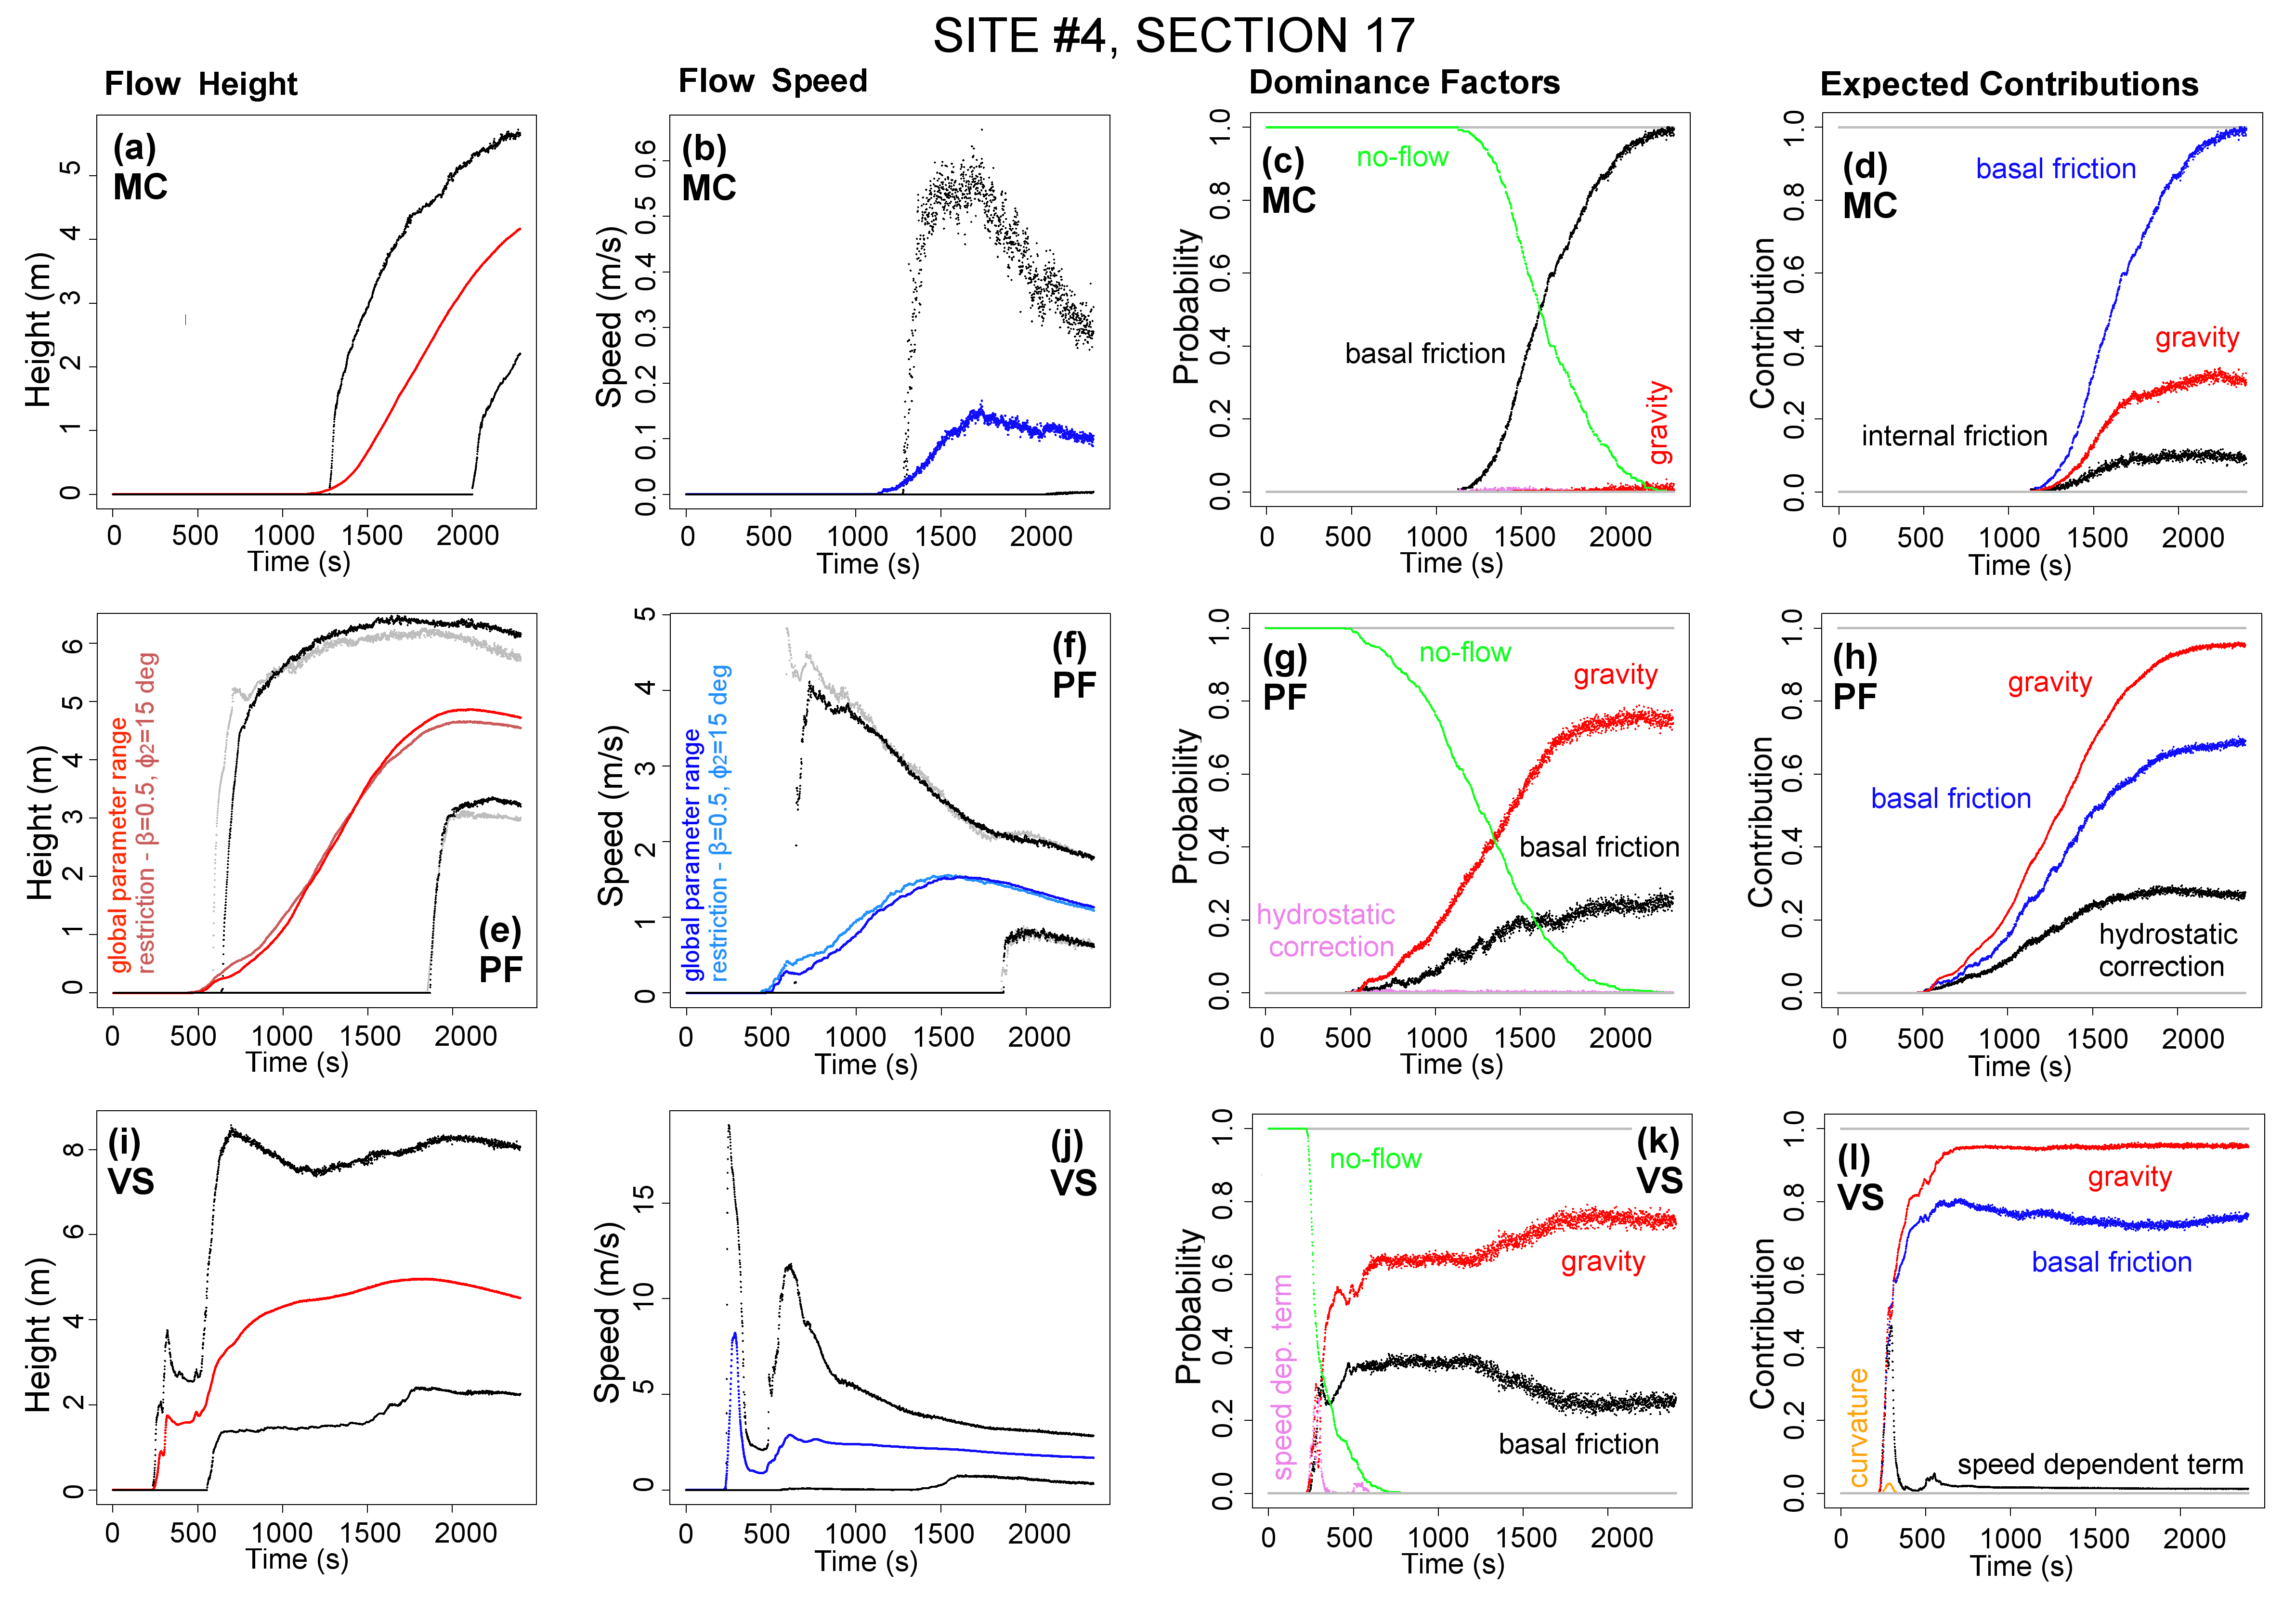
\includegraphics[width=0.97\textwidth]{Fig6.png}
\caption{Local flow properties in Site \#4, immediately before Atenquique village. (a,e,i) show flow height, (b,f,j) flow speed, (c,g,k) dominance factors, (d,h,l) expected contributions of the force terms. Different models are plotted separately: (a-d) assume MC; (e-h) assume PF, and (e,f) include estimates on a hyperplanar restriction of the input domain; (i-l) assume VS. In (a,b,e,f,i,j) colored line is mean value, black/gray lines are 5$^{\mathrm{th}}$ and 95$^{\mathrm{th}}$ percentile bounds.}
\label{Fig6}
\end{figure}
In summary, MC is characterized by a lower speed, and by the dominance of basal friction. The expected contribution of the internal friction is not negligible, meaning the internal shear of the material is important. In PF, the pressure force contribution is significant, and it can even be the dominant force initially. This is related to the steepening of the flow front. An initial short lasting wave of hight speed is observed in either PF or VS, as is particularly evident in the upper bound of the plots. This fast wave is related to the closest source, \#3. The uncertainty affecting height and speed is generally higher in VS than in PF, in spite of the higher dimensionality of the second.

Figure \ref{Fig6} shows the local properties at site \#4, located immediately upstream from Atenquique village. In MC, the flow reaches the site in $[1300,\ 2100]$ s, with a flow height of $[2,\ 5.5]$ m. Flow speed is $<0.6\ m/s$, and $0.1\ m/s$, on average. Only basal friction is dominant, with the gravitational force being 30\% of basal friction, and internal friction 10\%, on average. In PF, the flow reaches the site at $[600,\ 1800]$ s, with a flow height of $[3,\ 6]$ m, which is stable in time. Flow speed is initially in $[1,\ 4]\ m/s$ and half of these values are at $t_f$. Either basal friction or gravity can be dominant. Gravitational force can be 95\% of the expected contribution, while basal friction is 65\%, and the pressure force, 25\%. In VS, the flow reaches the site in $[250,\ 550]$ s, with a first wave of $<3$ m. A second wave of $[1.5,\ 8]$ m arrives, and stays stable in depth. Flow speed also shows two waves - it is $<19\ m/s$, initially, then rises to $<12\ m/s$, with a gap in the middle. It is $[1,\ 3]\ m/s$ at $t_f$. Either gravity or basal friction can be dominant, with 95\% and 80\% of the expected contribution, respectively. In the initial fast wave, the speed dependent friction can be dominant, with 25\% of the expected contribution.  In summary, all the models show lower flow height and speed than at the previous site upstream. The flow depth is stable, without decreasing downstream, meaning no formation of a significant deposit. MC is much slower than the other models, and its dynamics is completely dominated by basal friction. An initial, short-lasting wave of high speed is observed in VS. This fast wave is related to source \#5 in Arroyo Plat\'anos.
\begin{figure}[H]
\centering
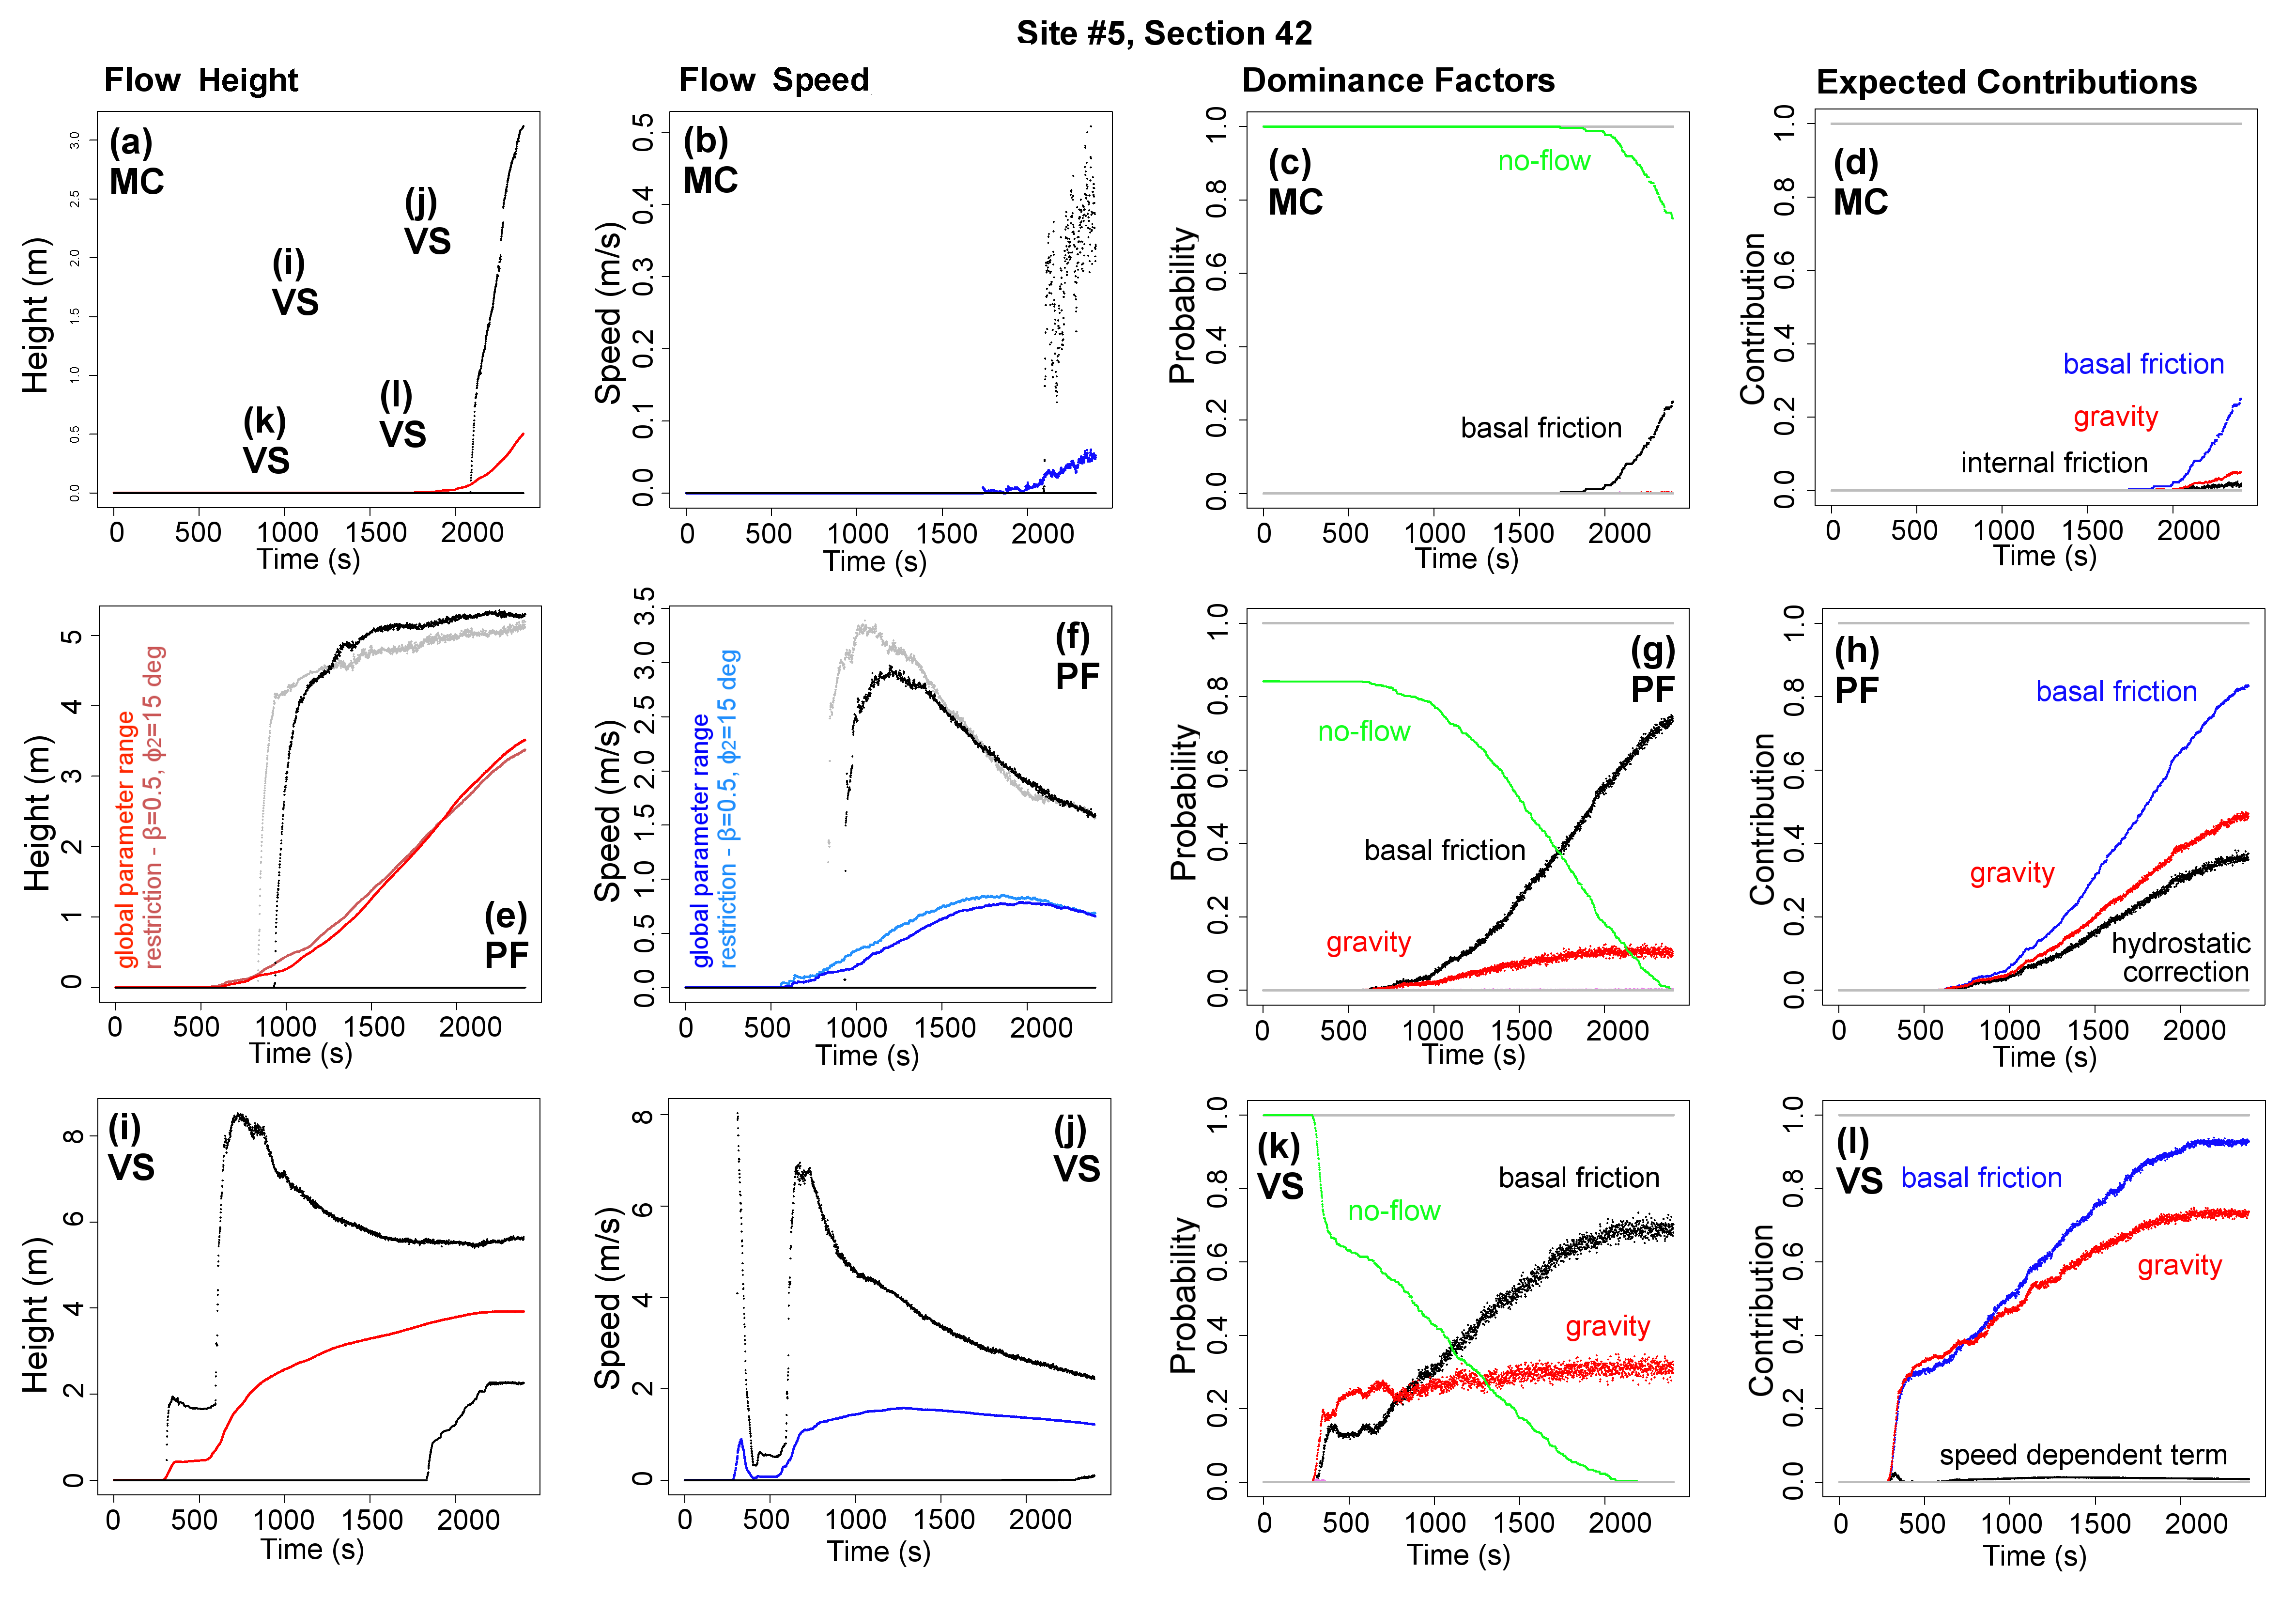
\includegraphics[width=0.97\textwidth]{Fig7.png}
\caption{Local flow properties in Site \#5, $\sim$1 km downstream inside Atenquique village. (a,e,i) show flow height, (b,f,j) flow speed, (c,g,k) dominance factors, (d,h,l) expected contributions of the force terms. Different models are plotted separately: (a-d) assume MC; (e-h) assume PF, and (e,f) include estimates on a hyperplanar restriction of the input domain; (i-l) assume VS. In (a,b,e,f,i,j) colored line is mean value, black/gray lines are 5$^{\mathrm{th}}$ and 95$^{\mathrm{th}}$ percentile bounds.}
\label{Fig7}
\end{figure}
Figure \ref{Fig7} shows the local properties at site \#5, $\sim$1 km downstream from site \#4, inside the bounds of Atenquique village. In MC, the flow only starts to inundate the site after $2100$ s, with a flow height $<3$ m. Flow speed is $<0.5\ m/s$, and ten times lower on average. Only basal friction can be dominant. In PF, the flow reaches the site at $[900,\ 2400]$ s, with a flow height $<5$ m. Flow speed is initially $<3\ m/s$, and less than half of this value at $t_f$. Basal friction dominates the dynamics, with 45\% expected contribution from the gravitational force, and 35\% from the pressure force. In VS, the flow reaches the site in $[300,\ 600]$ s, with a first wave of $<2$ m, and then a second wave $<8$ m. This second wave becomes $[2,\ 5.5]$ m at $t_f$. Flow speed is $<8\ m/s$ in the first wave, and then $<7\ m/s$ in the second, with a gap in the middle. The average speed is stable at $1.5\ m/s$. Either basal friction or gravity can dominate, with 95\% and 70\% expected contributions, respectively.  In summary, the models show a decrease in flow height and speed compared to the previous site. In MC, the site is not always reached, and in PF some input values inundate the site only at the end of the time domain. In PF,  restriction of the inputs over a lower dimensional subspace produces a lag of about $100$ s, possibly motivated by a fixed value of $\phi_2=15^\circ$ being higher than the middle of its variable range. The fast wave in VS is again related to source \#5.

\section{The likelihood of a model given uncertain data}\label{s4}
Figures \ref{Fig8} and \ref{Fig9} show the flow height and speed histograms at the three selected sites, either their maximum value, or  their value at $t=2400$ s. These confirm what is summarized in the previous section. The following probability density values  are evaluated with respect to m and m/s, respectively. In Figure \ref{Fig8}:
\begin{itemize}
\item\textbf{Site \#3} Flow height pdf at $t_f$ is above $0.1$ over: $[3,\ 5.5]$ m in MC, $[2,\ 4.5]$ m in PF and $[1.5,\ 4.5]$ m in VS. The first two models are more peaked, while the third produces a tail of very large thickness values, up to $8$ m. The maximum height pdf is above $0.1$ over: $[5.5,\ 8]$ m in MC, $[6,\ 9]$ m in PF, $[8,\ 13]$ in VS.
\item\textbf{Site \#4} Flow height pdf at $t_f$ is above $0.1$ over: $[2.5,\ 6]$ m in MC, $[3,\ 6]$ m in PF and $[2,\ 7]$ m in VS. The maximum height pdf is above $0.1$ over: $[2.25,\ 6]$ m in MC, $[5,\ 7]$ m in PF, $[6,\ 9.5]$ m in VS. The three models show well separate modal values at $4$, $6$ and $8$ m, respectively.
\item\textbf{Site \#5} In MC and PF do not always reach the site in $T=[0,\ 2400]$ s, so they both show a modal value of flow height in $0$ m. The flow height pdf at $t_f$ is above $0.1$ over: $[1,\ 1.5]$ m in MC with a tail up to $3.5$ m, $[3,\ 5.5]$ m in PF, $[2,\ 6]$ m in VS. The maximum height pdf is almost equal to final height in MC, and it is above $0.1$ over: $[3.5,\ 6]$ m in PF, $[3.5,\ 9]$ m in VS. Both PF and VS show a modal value at $5$ m.
\end{itemize}
In Figure \ref{Fig9}:
\begin{itemize}
\item\textbf{Site \#3} Flow speed pdf at $t_f$ is above $0.25$ over: $[0.1,\ 1.4]$ m/s in MC, $[1.6,\ 2.4]$ m/s in PF and $[1.4,\ 2.8]$  m/s in VS. MC is bimodal at $0.5$ m/s and $1$ m/s, while PF has a modal value at $2.1$ m/s. The maximum speed pdf is above $0.05$ over: $[1,\ 7]$ m/s in MC, $[4,\ 8]$ m in PF, $[4,\ 16]$ in VS. PF and VS have tails up to $25$--$30$ m/s.
\item\textbf{Site \#4} Flow speed pdf at $t_f$ is above $0.25$ over: $[0.00,\ 0.45]$ m/s in MC, $[0.6,\ 1.8]$ m/s in PF and $[0.5,\ 3.0]$  m/s in VS. PF has a modal value at $1$ m/s. Maximum speed pdf in MC is concentrated below $1$ m/s. In PF, it is above $0.25$ over $[1,\ 5]$ m/s. In VS, it is bimodal and above $0.25$ over: $[2,\ 6]$ m/s and $[12, 20]$ m/s.
\item\textbf{Site \#5} Flow speed pdf at $t_f$ is above $0.25$ over: $[0.0,\ 0.4]$ m/s in MC, $[0.0,\ 1.4]$ m/s in PF and over $[0.0,\ 0.2]$ and $[0.4,\ 2.2]$  m/s in VS. The maximum speed pdf is above $0.05$ over: $[0.0,\ 0.2]$ and $[0.4,\ 1.2]$ m/s in MC, to $[0,\ 4]$ m in PF, $[0,\ 9]$ in VS. PF and VS have tails up to $8$ and $13$ m/s, respectively.
\end{itemize}

\subsection{Alternative performance scores of the models}
In  Figures \ref{Fig8} and \ref{Fig9}, we display the empirical data concerning the observed quantities. These intervals are examples of uncertain data to test our methodology. Further research could refine/modify them.
\begin{figure}[H]
\centering
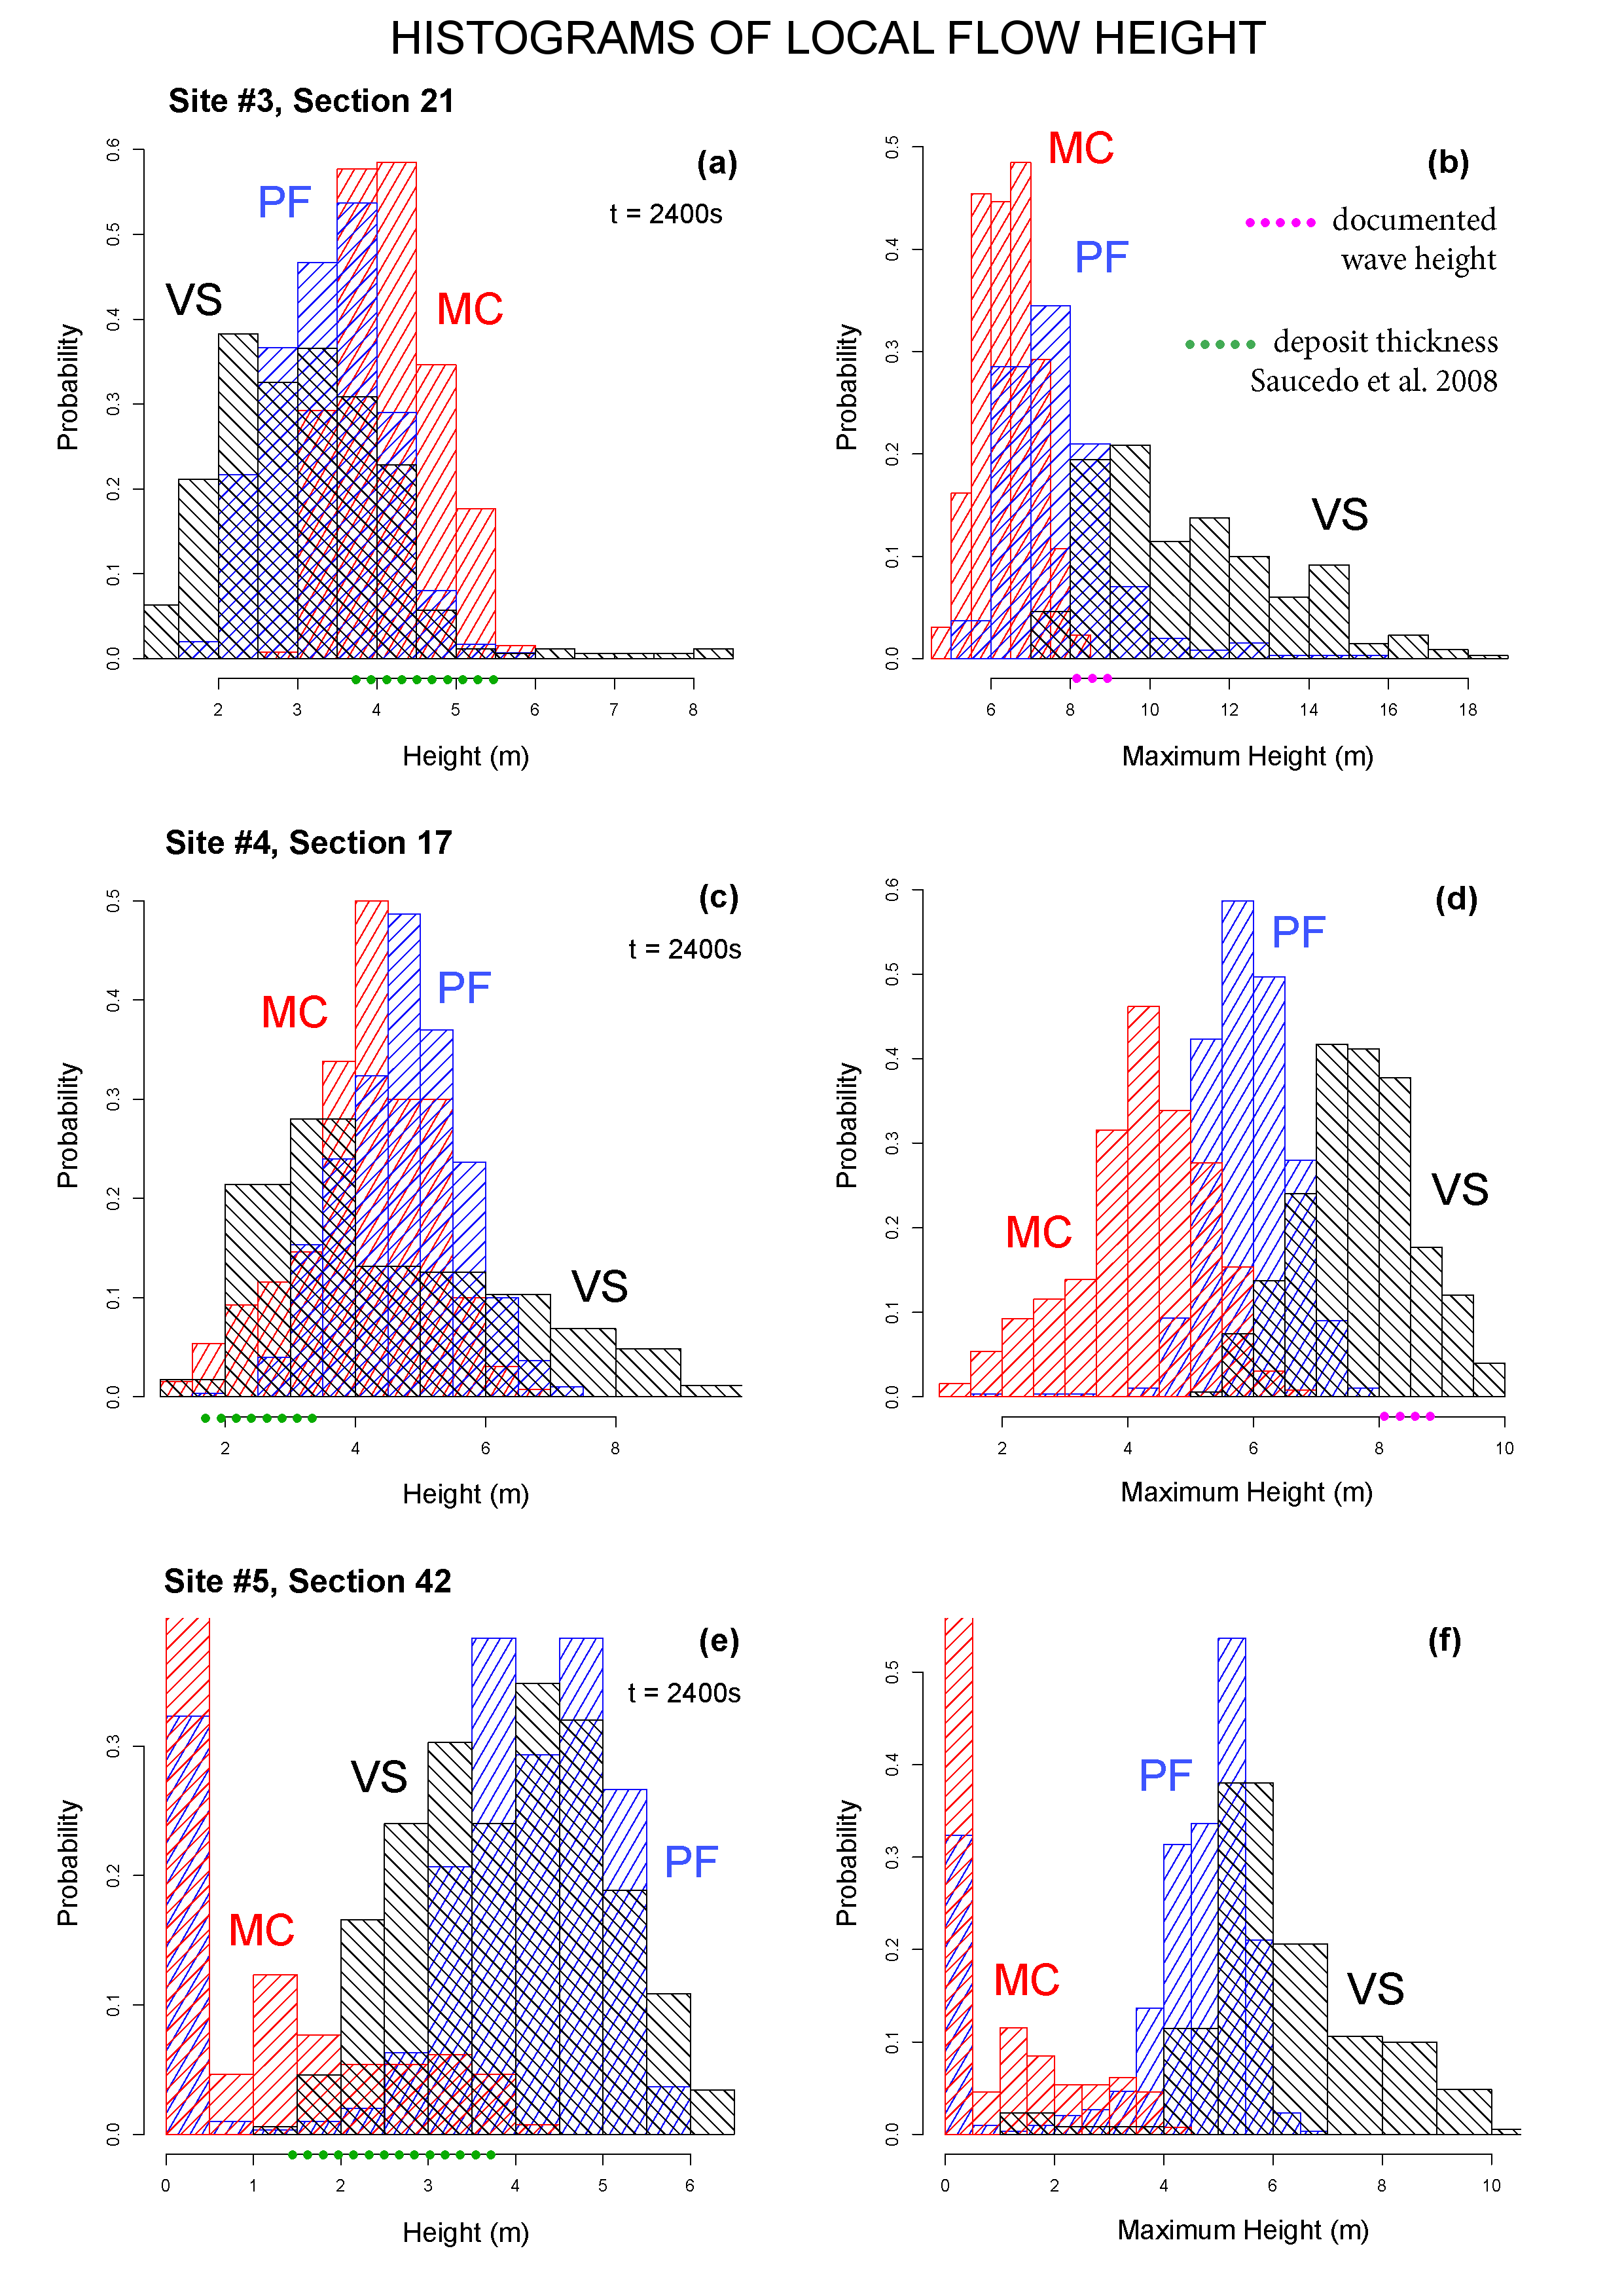
\includegraphics[width=0.85\textwidth]{Fig8.png}
\caption{Histograms of local flow height in Sites \#3,\#4, \#5. (a,c,e) show height at $t=2400$ s, (b,d,f) maximum height. Different models are displayed with different colors. Dots on the height axis show the uncertainty interval of data - green is the deposit thickness of \cite{Saucedo2008} and unpublished data, violet is the wave height documented by the survivors.}
\label{Fig8}
\end{figure}

\begin{figure}[H]
\centering
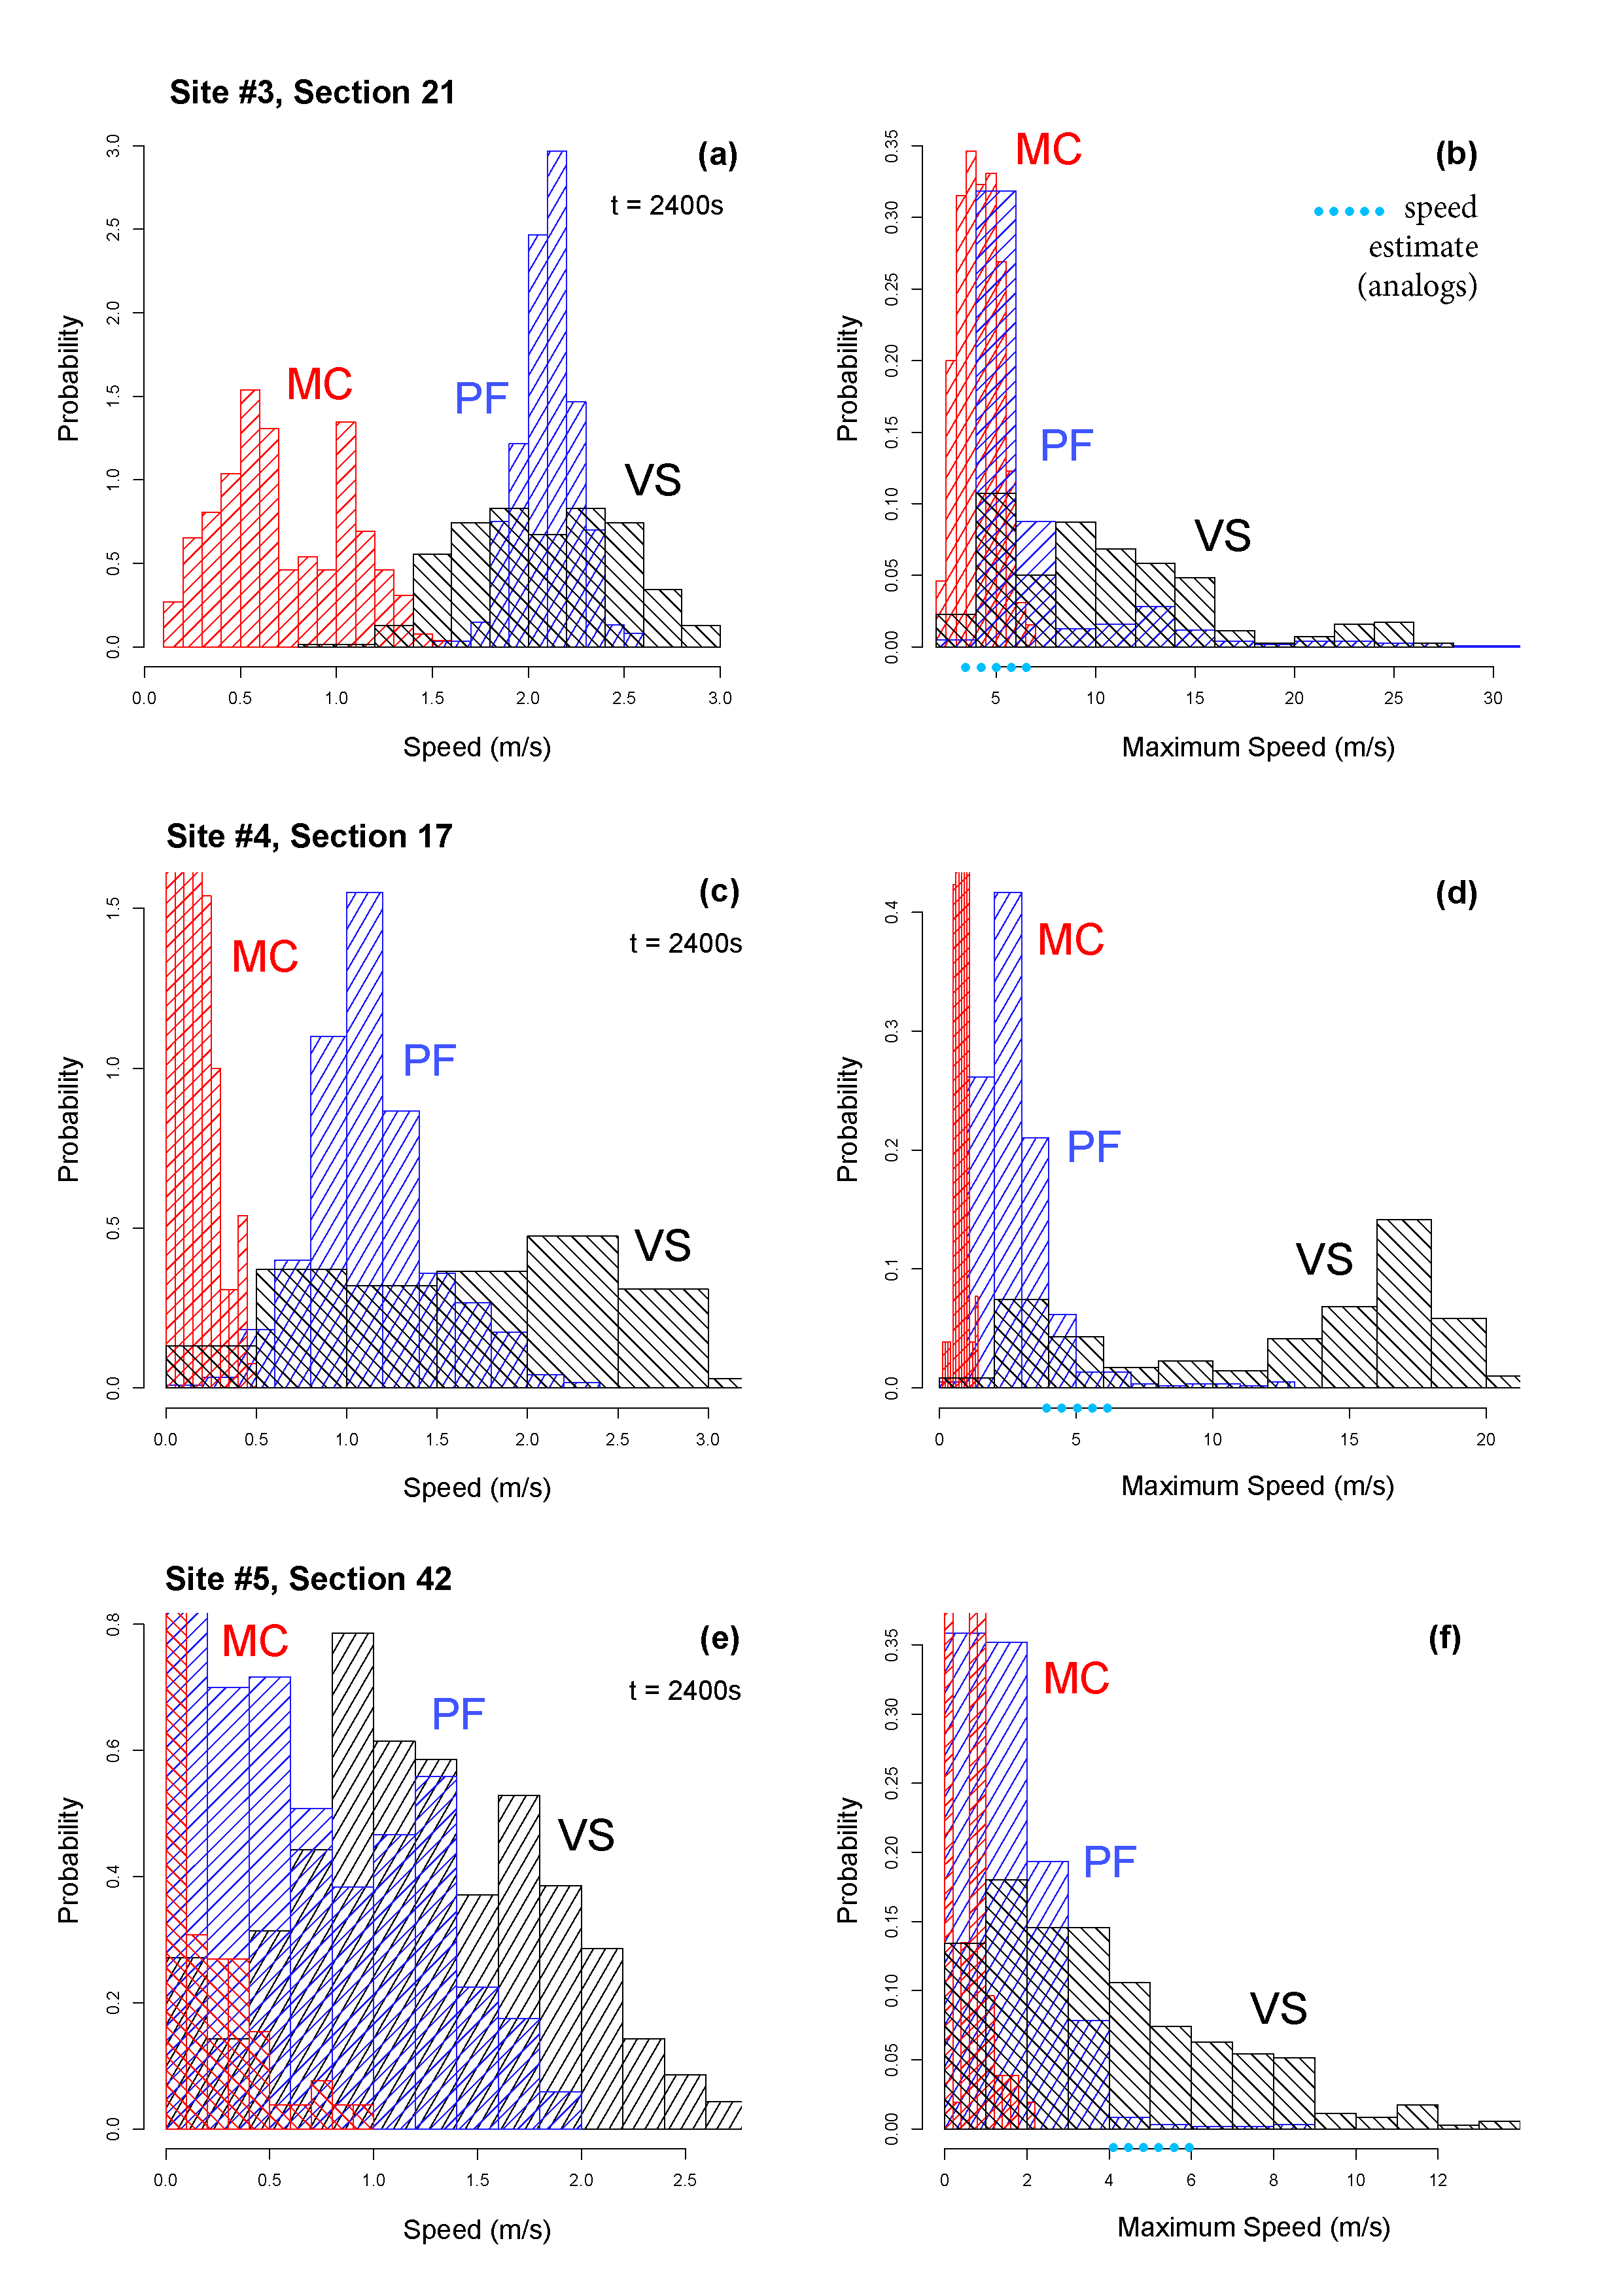
\includegraphics[width=0.85\textwidth]{Fig9.png}
\caption{Histograms of local flow speed in Sites \#3,\#4, \#5. (a,c,e) show speed at $t=2400$ s, (b,d,f) maximum speed. Different models are displayed with different colors. Cyan dots on the speed axis show the uncertainty interval of estimated speed \cite{Pierson1985}.}
\label{Fig9}
\end{figure}

\begin{figure}[H]
\centering
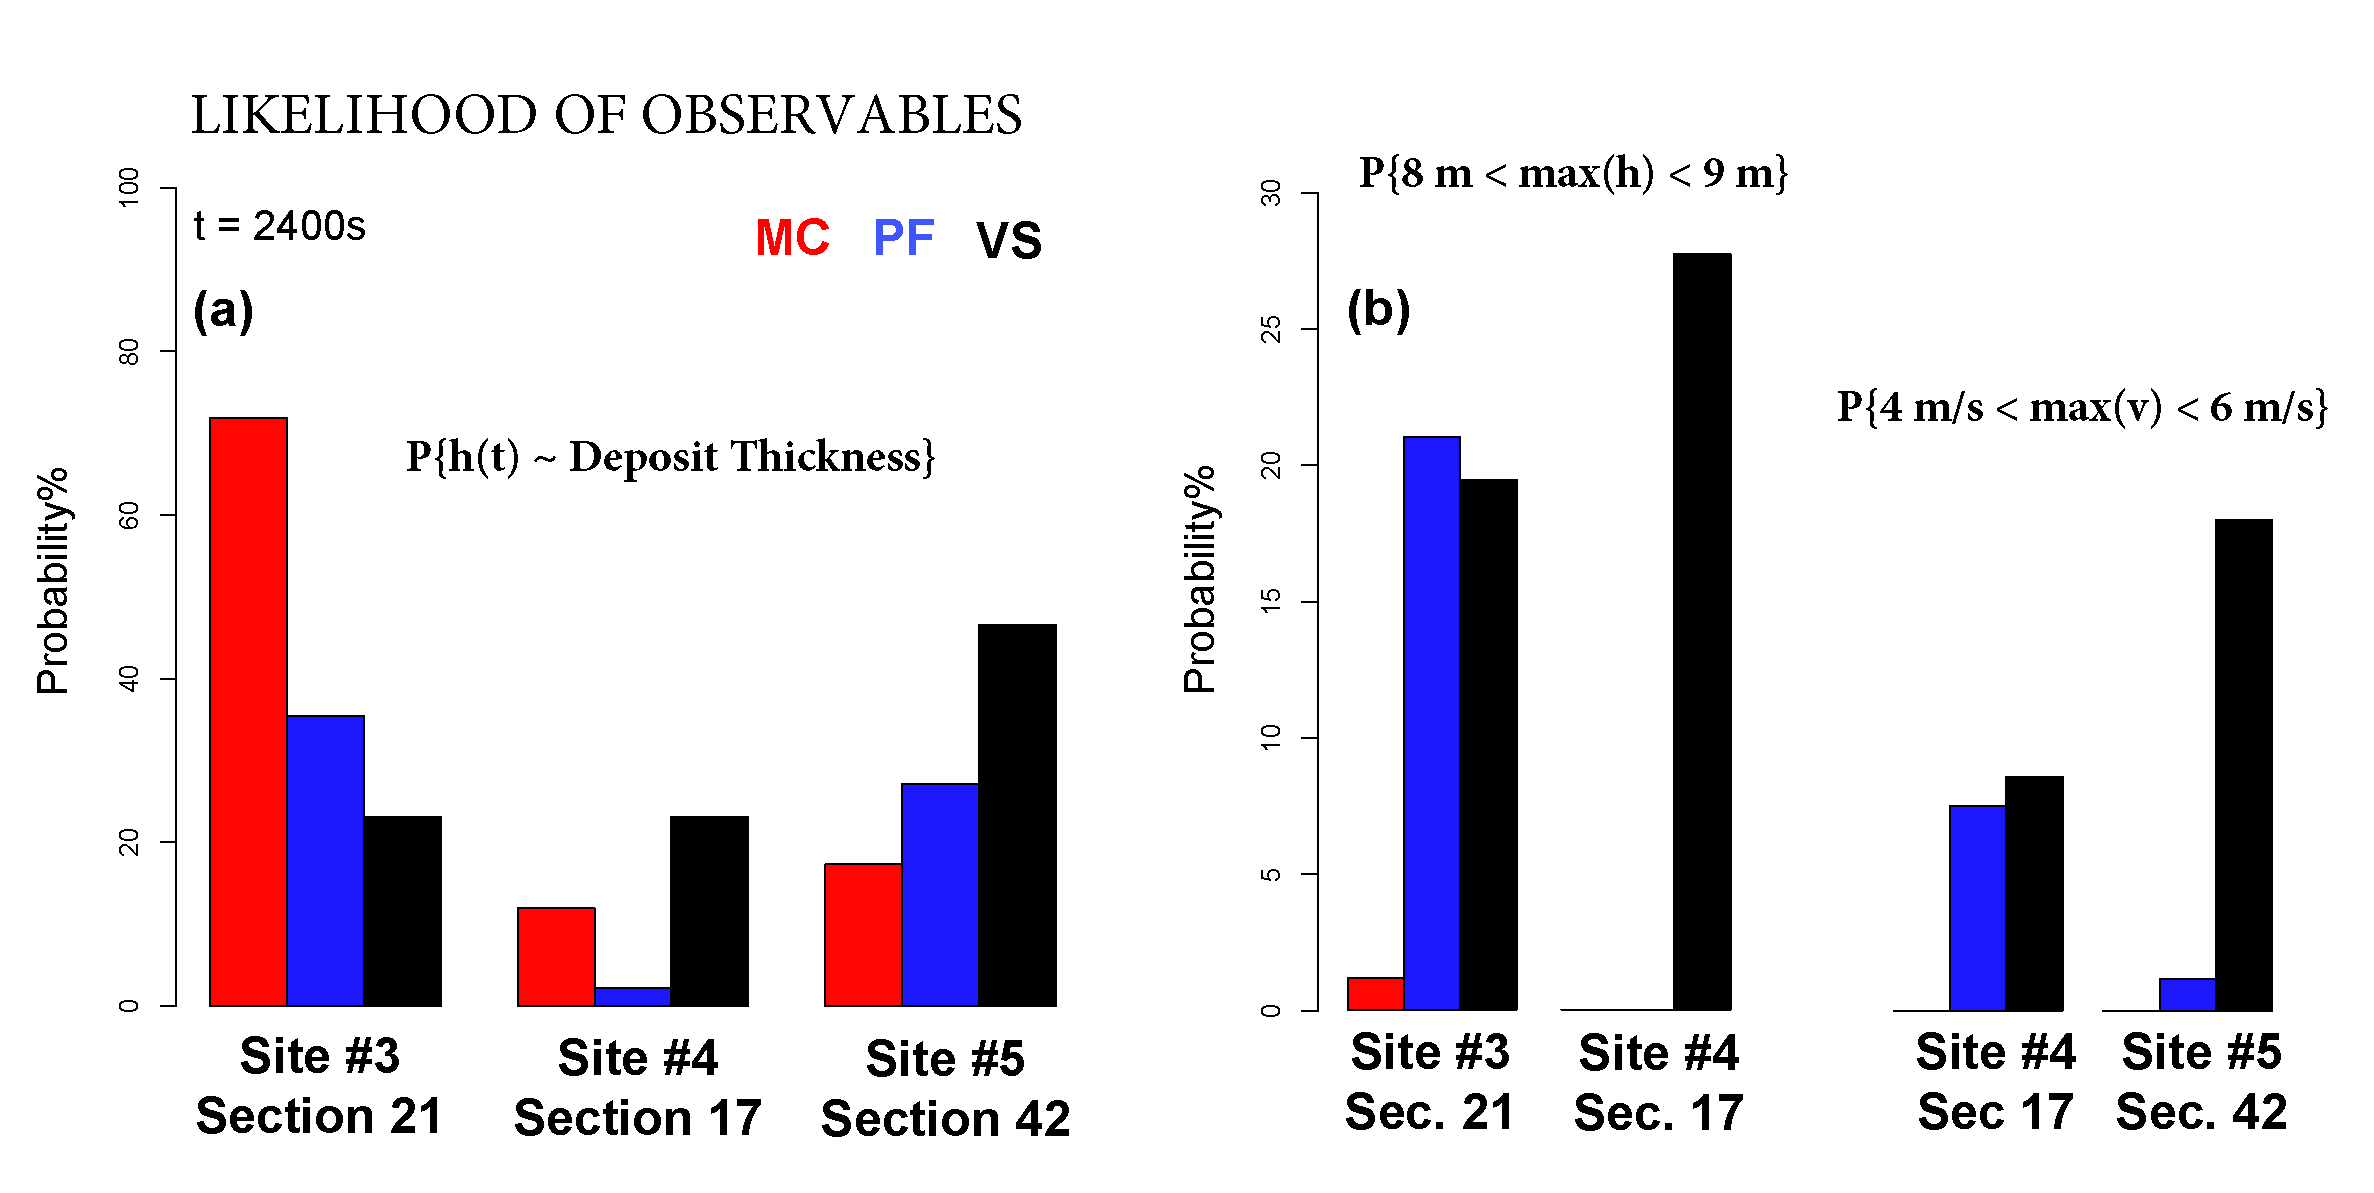
\includegraphics[width=1\textwidth]{Fig10.png}
\caption{Barplots of data likelihood in Sites \#3, \#4, \#5. (a) compares flow height at $t=2400$ s with observed deposit thickness \citep{Saucedo2008}. (b) compares maximum height and maximum speed with observed wave height \citep{PonceSegura1983} and analog flow speed \citep{Pierson1985}. Different models are displayed with different colors.}
\label{Fig10}
\end{figure}
\begin{enumerate}
\item The deposit thickness, calculated from the envelope of the closest field sections, is \\ $[3.7,\ 5.5]$ m at \textbf{Site \#3}, $[1.7,\ 3]$ m at \textbf{Site \#4}, and $[1.4,\ 3.8]$ m at \textbf{Site \#5} \citep{Saucedo2008}.
\item the flow height in Atenquique village, from historical documents and witnesses, is \\$[8,\ 9]$ m at \textbf{Site \#3} and/or \textbf{Site \#4} \citep{PonceSegura1983, Saucedo2008}.
\item The flow speed following the inundation of the village, based on a comparison with analog flows, is \\$[4,\ 6]\ m/s$ at \textbf{Site \#4} and/or \textbf{Site \#5} \citep{Pierson1985, Saucedo2008}.
\end{enumerate}
The estimation of the likelihood of the data points is an essential step towards the definition of partial solutions of the inverse problem. Besides this, it is also relevant information in the model selection problem. The likelihood of a data point, $D_i$, attaining its value given a certain model is defined as $P^j(D_i)$, $\forall i\in I$, $\forall M_j\in \mathcal M$. We remark that this is not a pdf value, but the probability of a measurable set. Figure \ref{Fig10} shows the barplots of data likelihood. Figure \ref{Fig10}a considers deposit thickness values, under the assumption that they are equivalent to the flow height at $t_f$. At Site \#3, 70\% of MC inputs provide flow thickness consistent with the deposit range, against 35\% of PF and 20\% of VS inputs. At Site \#4, likelihood scores are lower: 20\% in MC, 10\% in VS, $<$5\% in PF. At Site \#5, instead, we have: 15\% in MC, 25\% in PF, 45\% in VS. Figure \ref{Fig10}b evaluates the maximum flow height when the flow entered Atenquique village. In Site \#3, 20\% of inputs in PF and VS provide results consistent with data, while only $<$5\% do so in MC. At Site \#4, the likelihood score of VS is 27\%, while it is null in the other models. Figure \ref{Fig10}c focuses on the maximum flow speed after the flow inundated the village. At Site \#4, 8\% of inputs in PF and 9\% in VS provide speeds in the most likely range. At Site \#5, these are only 1\% in PF, and 17\% in VS.

In summary, model performance is dependent on the selected quantity of interest, and on the spatial location. Concerning the deposits, MC performs well at  Site \#3, while VS does so at Site \#5.  In the evaluation of the maximum flow depth in the village, both PF and VS can replicate the values at Site \#3, and only VS can replicate the values at Site \#4. If we focus on the maximum flow speed, at Site \#4 both PF and VS perform moderately well, while at Site \#5, only VS can provide speed values inside the assumed range.
\begin{figure}[H]
\centering
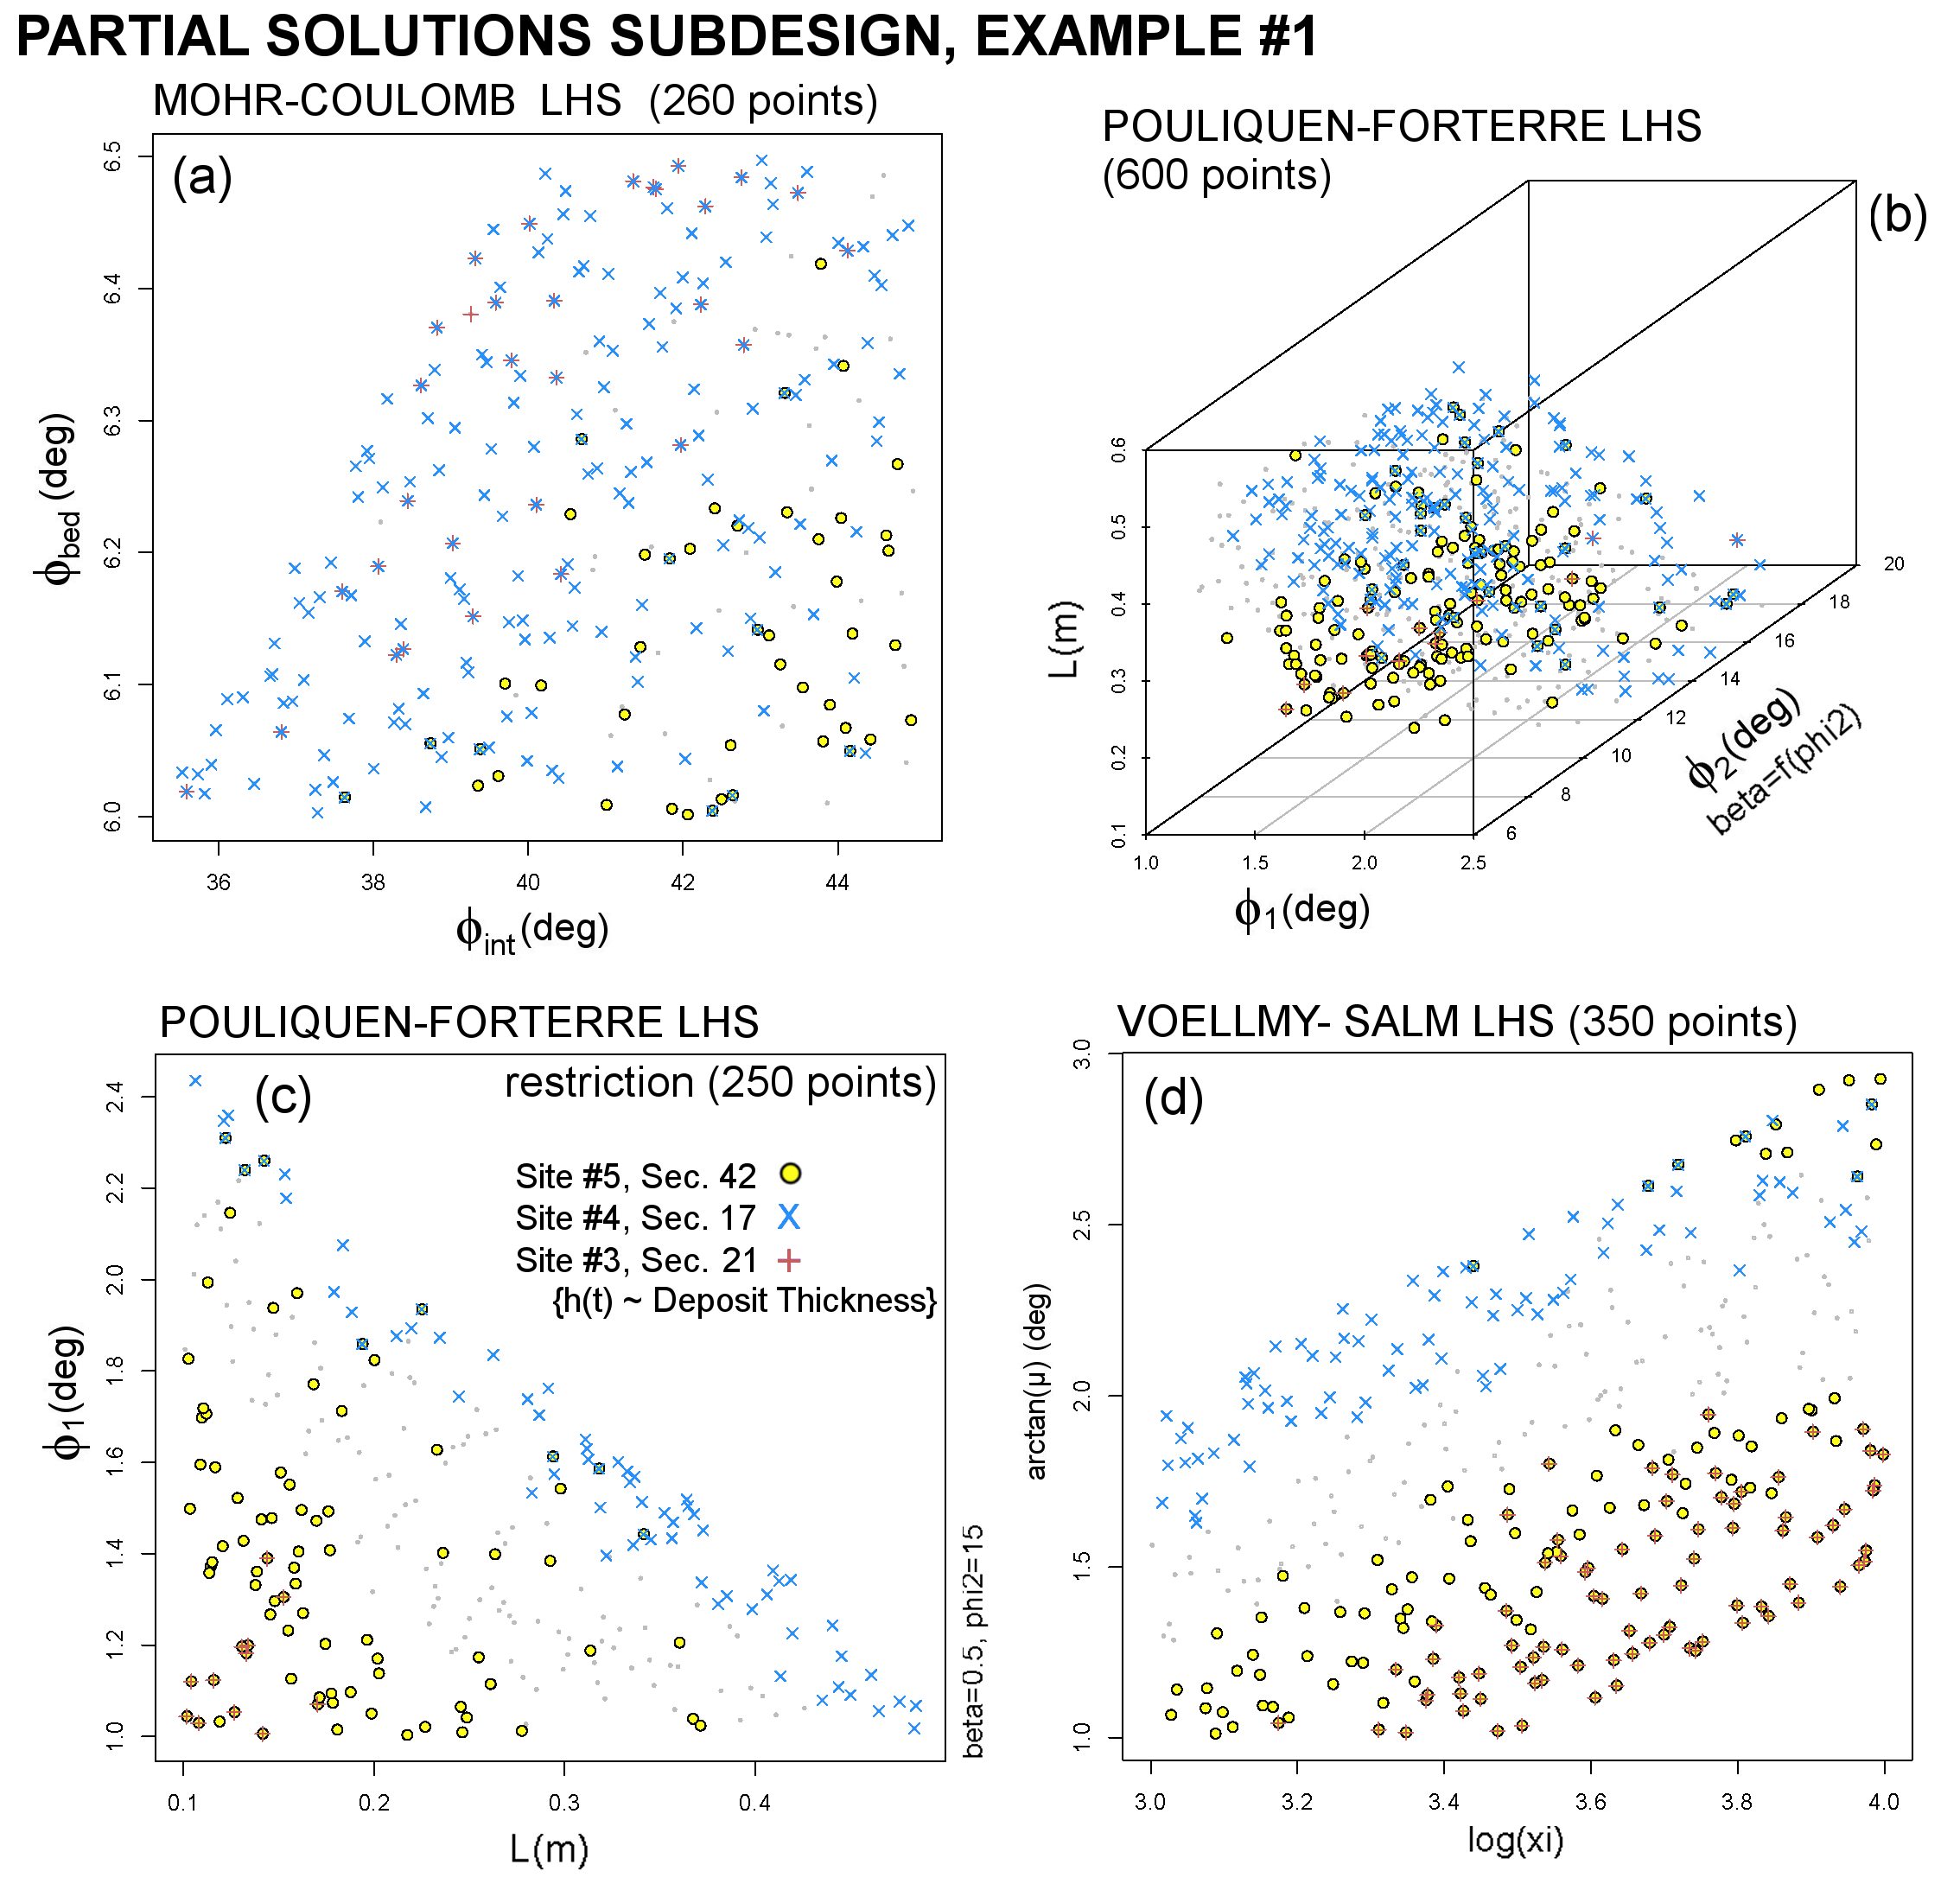
\includegraphics[width=0.82\textwidth]{Fig11_0.png}
\caption{Example \#1 of partial solution inputs in (a-b) MC, (c-d) PF, (e-f) VS experimental design. (a-c-e) are projected along the $V$ coordinate, and (b-d-f) along $\phi_{int}$, $\phi_2$ and $\xi$ coordinates, respectively. The color expresses the considered data: yellow is deposit thickness in Site \#5, blue in Site \#4, red in Site \#3 \citep{Saucedo2008}.}
\label{Fig11_0}
\end{figure}

\begin{figure}[H]
\centering
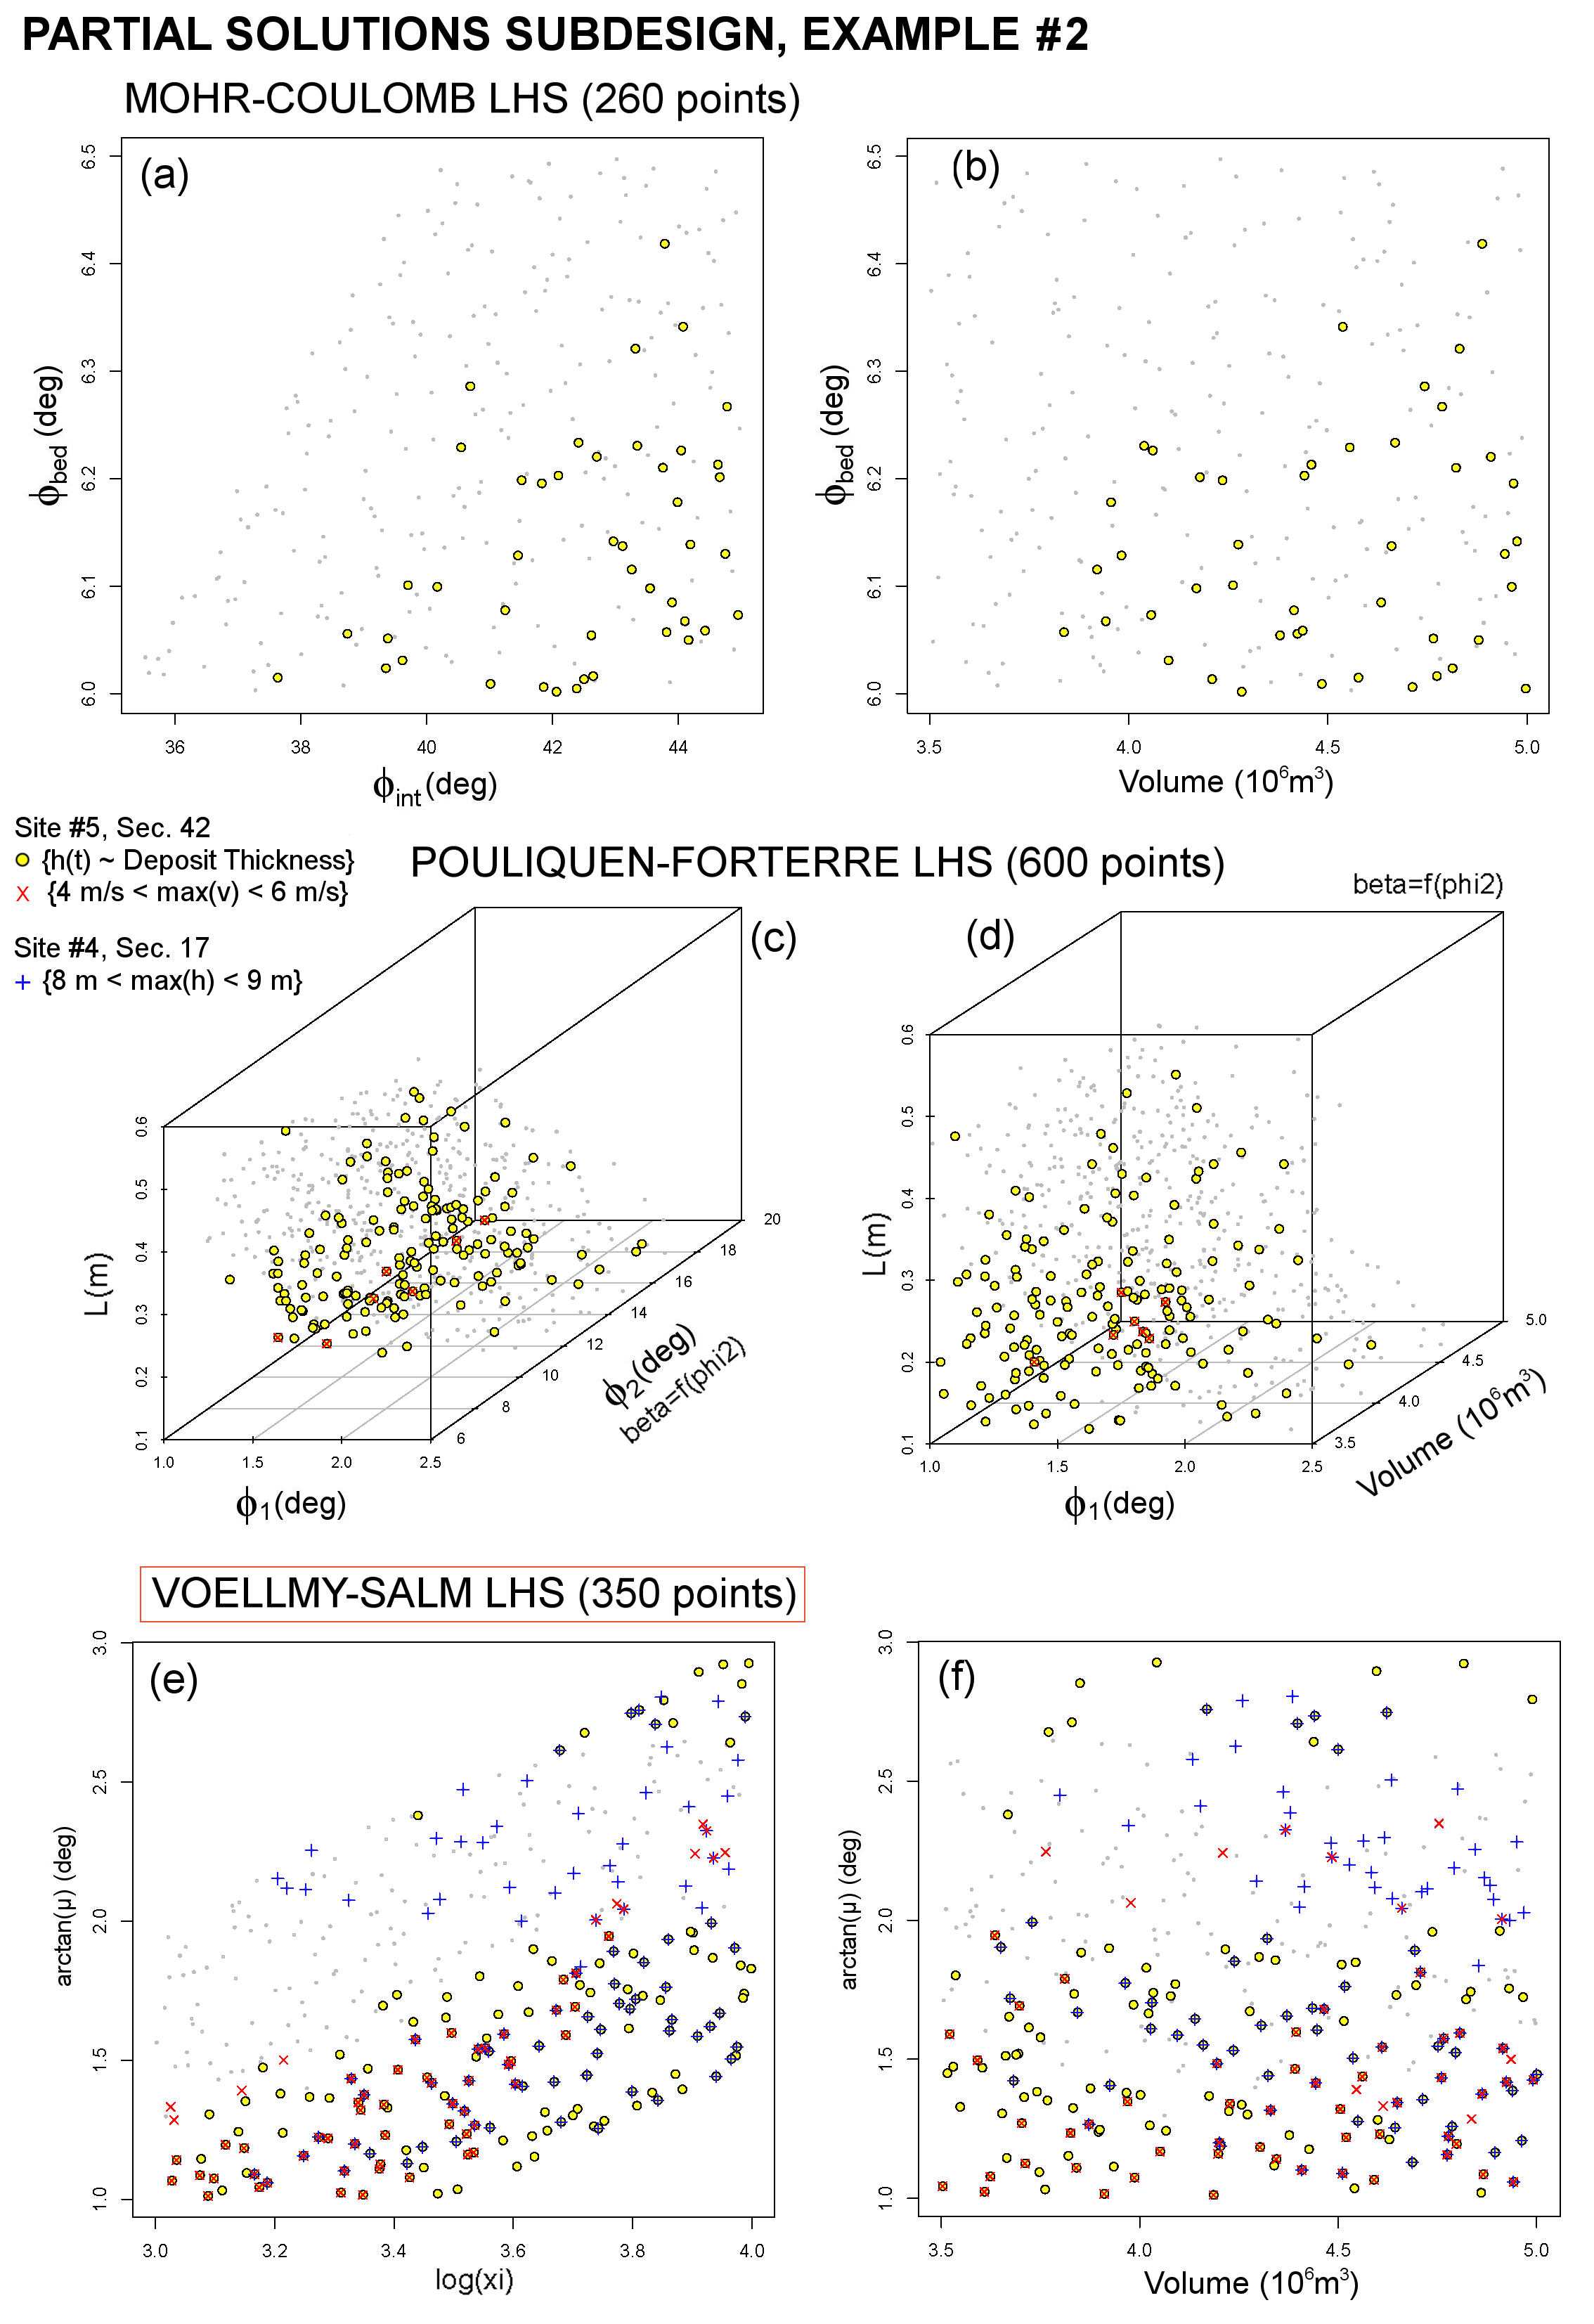
\includegraphics[width=0.82\textwidth]{Fig11.png}
\caption{Example \#2 of partial solution inputs in (a-b) MC, (c-d) PF, (e-f) VS experimental design. (a-c-e) are projected along the $V$ coordinate, and (b-d-f) along $\phi_{int}$, $\phi_2$ and $\xi$ coordinates, respectively. The color expresses the considered data: yellow is deposit thickness in Site \#5 \citep{Saucedo2008}, blue is wave height in Site \#4 \citep{PonceSegura1983}, red is flow speed in Site \#5 \citep{Pierson1985}.}
\label{Fig11}
\end{figure}

\begin{figure}[H]
\centering
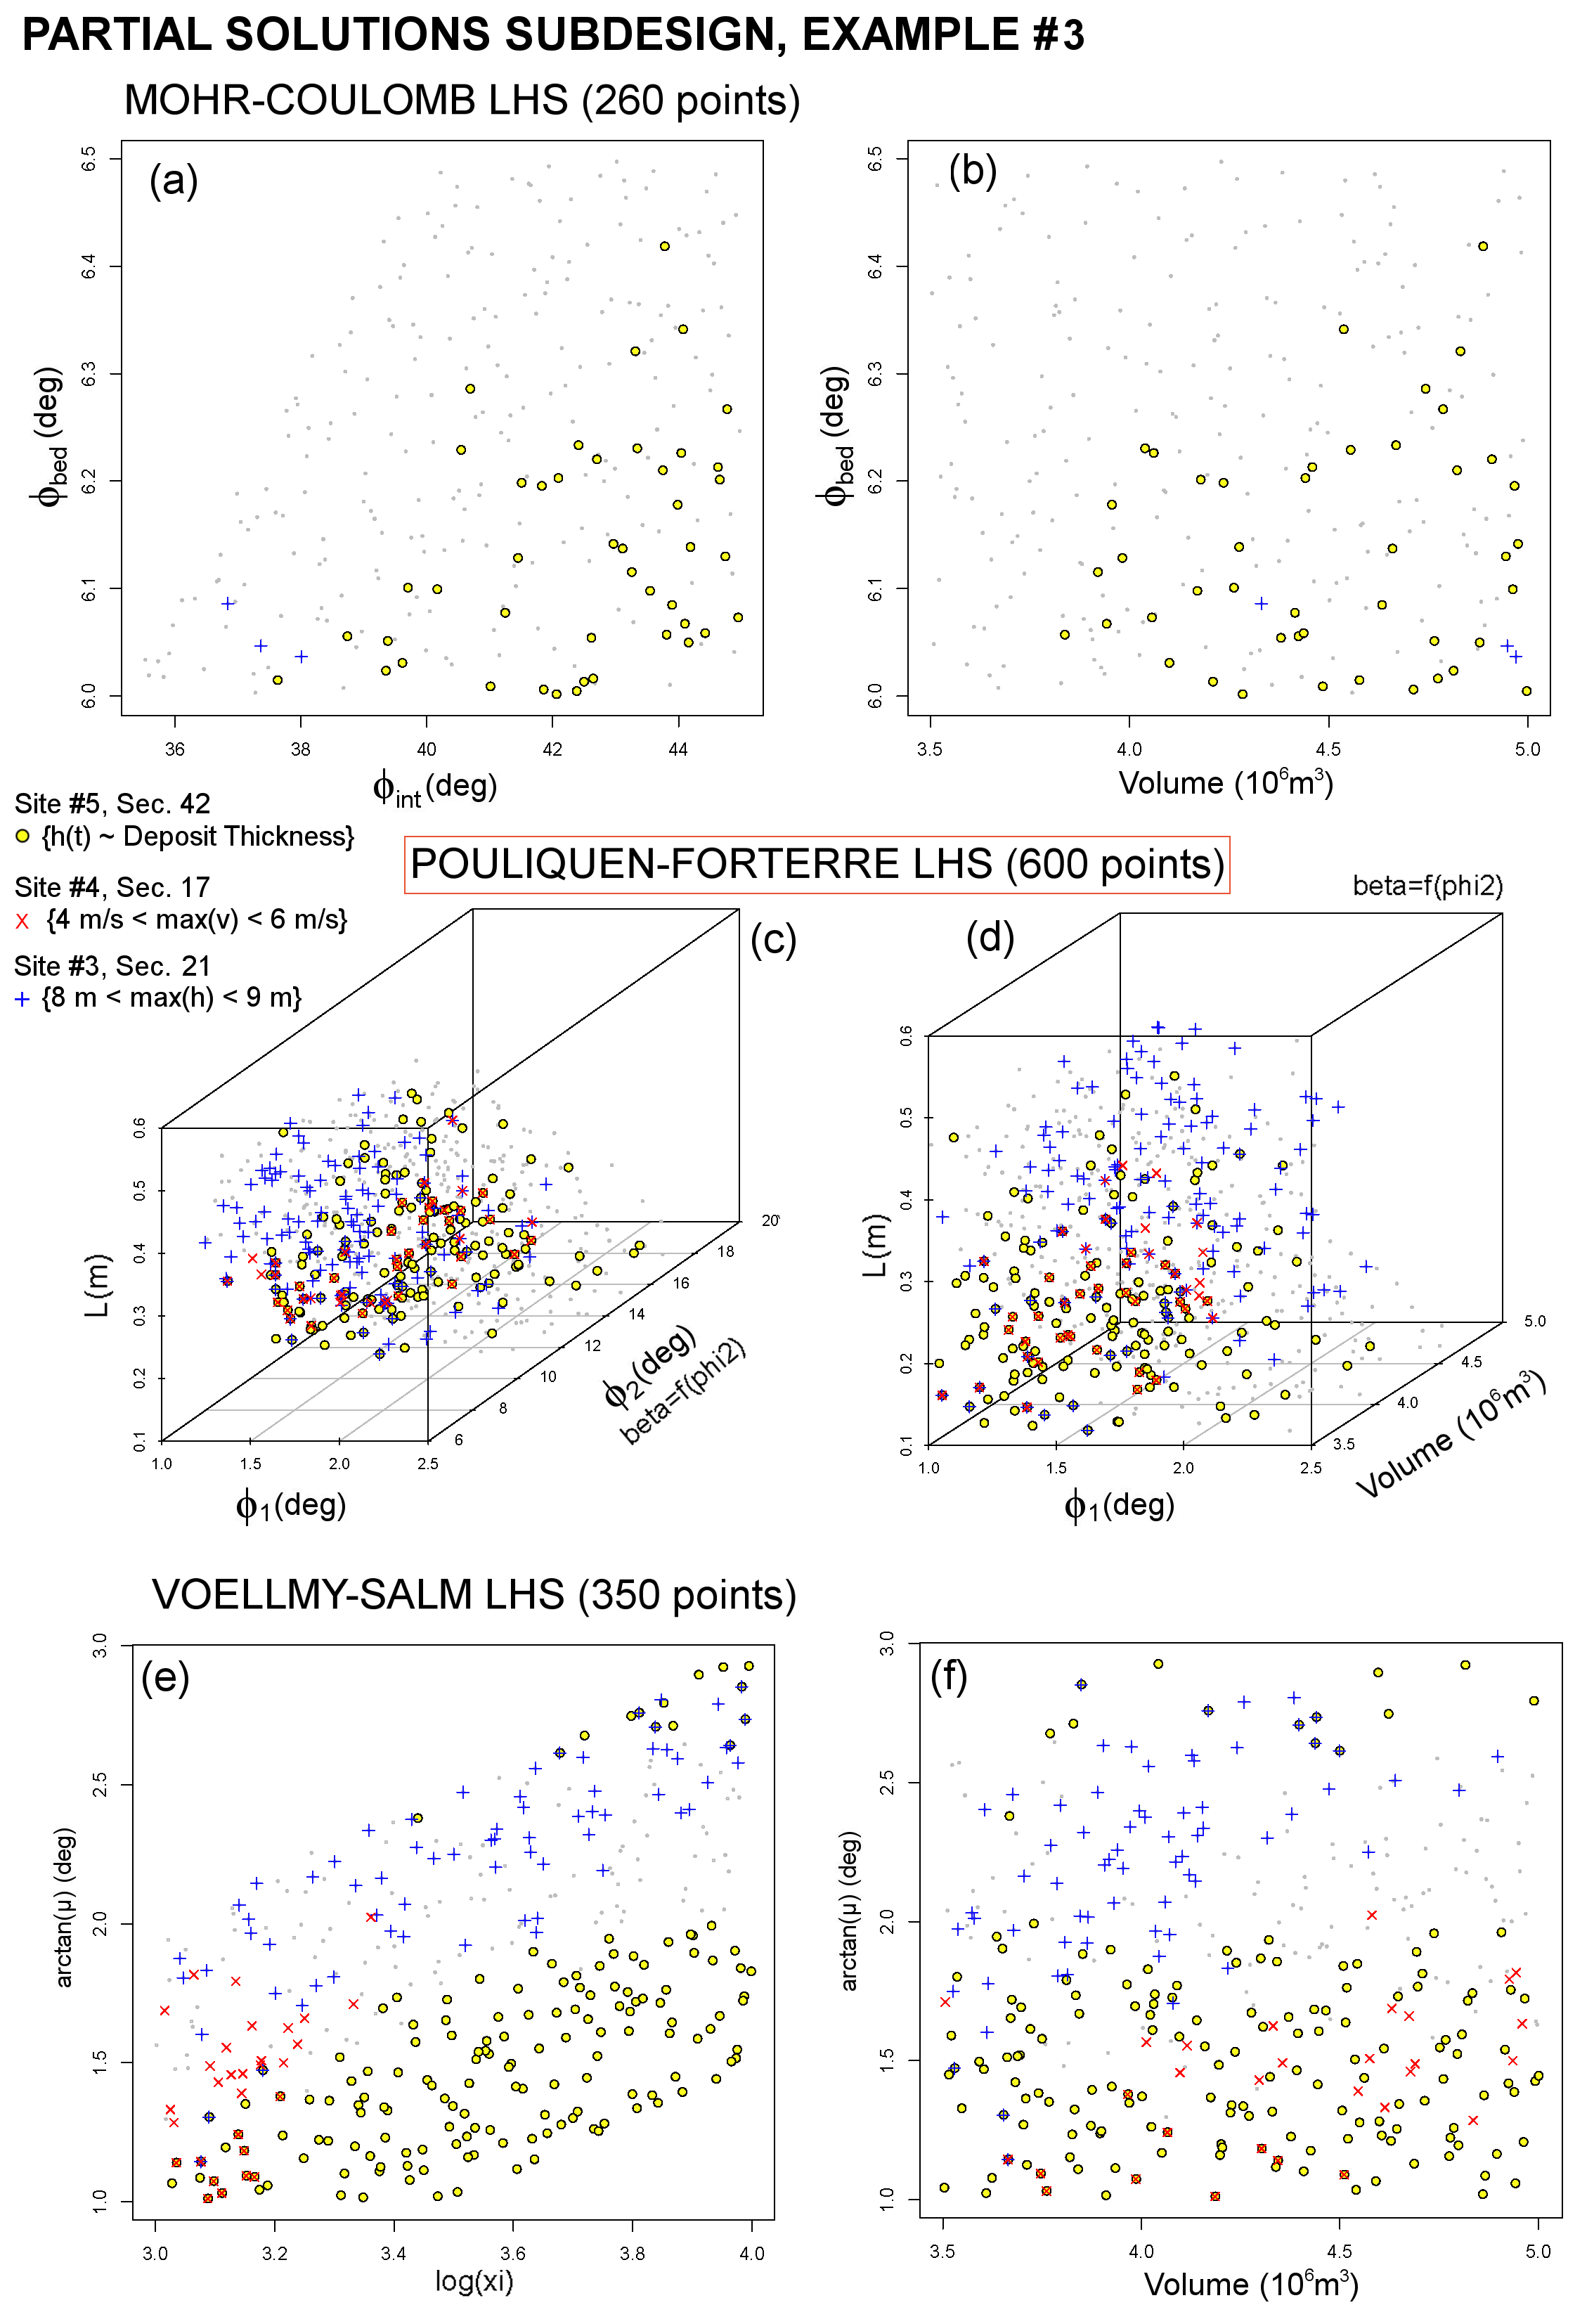
\includegraphics[width=0.82\textwidth]{Fig11_PF.png}
\caption{Example \#3 of partial solution inputs in (a-b) MC, (c-d) PF, (e-f) VS experimental design. (a-c-e) are projected along the $V$ coordinate, and (b-d-f) along $\phi_{int}$, $\phi_2$ and $\xi$ coordinates, respectively. The color expresses the considered data: yellow is deposit thickness in Site \#5 \citep{Saucedo2008}, blue is wave height in Site \#3 \citep{PonceSegura1983}, red is flow speed in Site \#4 \citep{Pierson1985}.}
\label{Fig11a}
\end{figure}
\section{Partial solutions in the input space}
Figures \ref{Fig11_0}, \ref{Fig11}, \ref{Fig11a} display three examples of partial solutions in the specialized experimental design.
For each example $n=1,2,3$ we select a subfamily of empirical data $(D_i)_{i\in I_n}$ and define, $\forall j$:
\begin{equation}
\tilde\Theta_n^j:=\bigcap_{i\in I_n} \Omega_i^j.
\end{equation}
Example \#1 focuses on the deposit thickness data at Sites \#3, \#4, \#5.  Examples \#2 and \#3 consider the deposit thickness at Site \#5 only. Additionally, Example \#2 evaluates the maximum flow height at Site \#4, and the maximum flow speed at Site \#5, while Example \#3 does that at Site \#3 and Site \#4, respectively.

Figure \ref{Fig11_0} concerns Example \#1. In all the models, $\tilde\Theta_1^j=\emptyset$. In MC, the set of inputs that replicate the deposit thickness at Site \#4 are disjoint from those in Site \#5. Instead, in PF and VS the inputs related to Site \#3 are disjoint from those related to Site \#4. Figure \ref{Fig11} concerns Example \#2. In MC and PF, the  maximum flow height from the data is never reproduced. In MC, the required maximum flow speed is never achieved. Thus, $\tilde\Theta_2^j\neq\emptyset$ only if $j=\textrm{VS}$. The partial solution inputs in $\tilde\Theta_2^{\textrm{VS}}$ are bounded by:
$$\arctan(\mu) \in [1.0,\ 1.8],\quad \xi\in[3.1, 3.7],\quad V \in [3.8,\ 5.0] \times 10^6\ m^3.$$ Figure \ref{Fig11a} is related to Example \#3. In MC, the required maximum flow speed from the data is never reproduced. We have that $\tilde\Theta_2^j\neq\emptyset$ for $j\in\{\textrm{PF}, \textrm{VS}\}$. In PF, the partial solution inputs in $\tilde\Theta_3^{\textrm{PF}}$ are bounded by:
$$\phi_1 \in [1.0,\ 1.6],\quad L \in [0.12,\ 0.25]\ m,\quad V \in [3.9,\ 4.9] \times 10^6\ m^3.$$
In VS, only one point belongs to the partial solution input set, with $\arctan(\mu) \simeq 1.2$, $\xi \simeq 3.1$, $V \simeq 3.6 \times 10^6$ $m^3$. Remarkably, the input spaces reproducing the three required pieces of empirical data are almost disjoint in pairs, and $\tilde\Theta_3^{\textrm{VS}}$ is small and close to the frontiers of the uncertainty ranges. Additional details in PF over the hyperplane $\{\beta=0.5,\ \phi_2=15\}$ described in Table 1 are included in Supporting Information SI6.

\subsection{Examples of conditional results}
The solution of the partial inverse problems can enable us to select a model, which nevertheless depends on the required properties and the spatial location. In particular:
\begin{itemize}
\item in Example \#1 the inverse problem is not well posed,
\item in Example \#2 only in VS can we find solutions: $\tilde\Theta_2^{\textrm{VS}}\neq\emptyset$,
\item in Example \#3 both in PF and VS we find solutions: $\tilde\Theta_3^{\textrm{PF}}\neq\emptyset$, $\tilde\Theta_3^{\textrm{VS}}\neq\emptyset$.
\end{itemize}
The points in the experimental design that belong to $\tilde\Theta_2^{\textrm{VS}}$ and $\tilde\Theta_3^{\textrm{PF}}$ are 21 and 9 respectively. We do not detail $\tilde\Theta_3^{\textrm{VS}}$ because it contains only one design point and the results can be disrupted even by relatively small variations of the inputs. Additional tests at a finer resolution in the experimental design could be performed to achieve a more accurate characterization of the conditional input spaces, if required.

In Figures \ref{Fig12} and \ref{Fig12a}, we report the histograms of:
$$K=\max_{t\in T}\kappa,\quad \kappa_f:=\kappa(t_f)\quad Q:=\max_{t\in T}\frac{\kappa}{h}$$
at Sites \#4 and \#5. The spatial maps of the maximum in flow height, $h$, and kinetic energy, $\kappa$, are also displayed. The \emph{dynamic pressure} $Q$ formally assumes a mass with unit density.

In Figure \ref{Fig12}, at Site \#4:
$$K\in[100,\ 400]\ m^3/s^2,\quad \kappa_f\in[4,\ 16]\ m^3/s^2,\quad Q\in[0,\ 150]\ m^2/s^2$$
and at Site \#5:
$$K\in[40,\ 140]\ m^3/s^2,\quad \kappa_f\in[0,\ 9]\ m^3/s^2,\quad Q\in[7.5,\ 17.5]\ m^2/s^2$$
The modal values of $K$ are $\sim 225\ m^3/s^2$ and $60\ m^3/s^2$, respectively.
\begin{figure}[H]
\centering
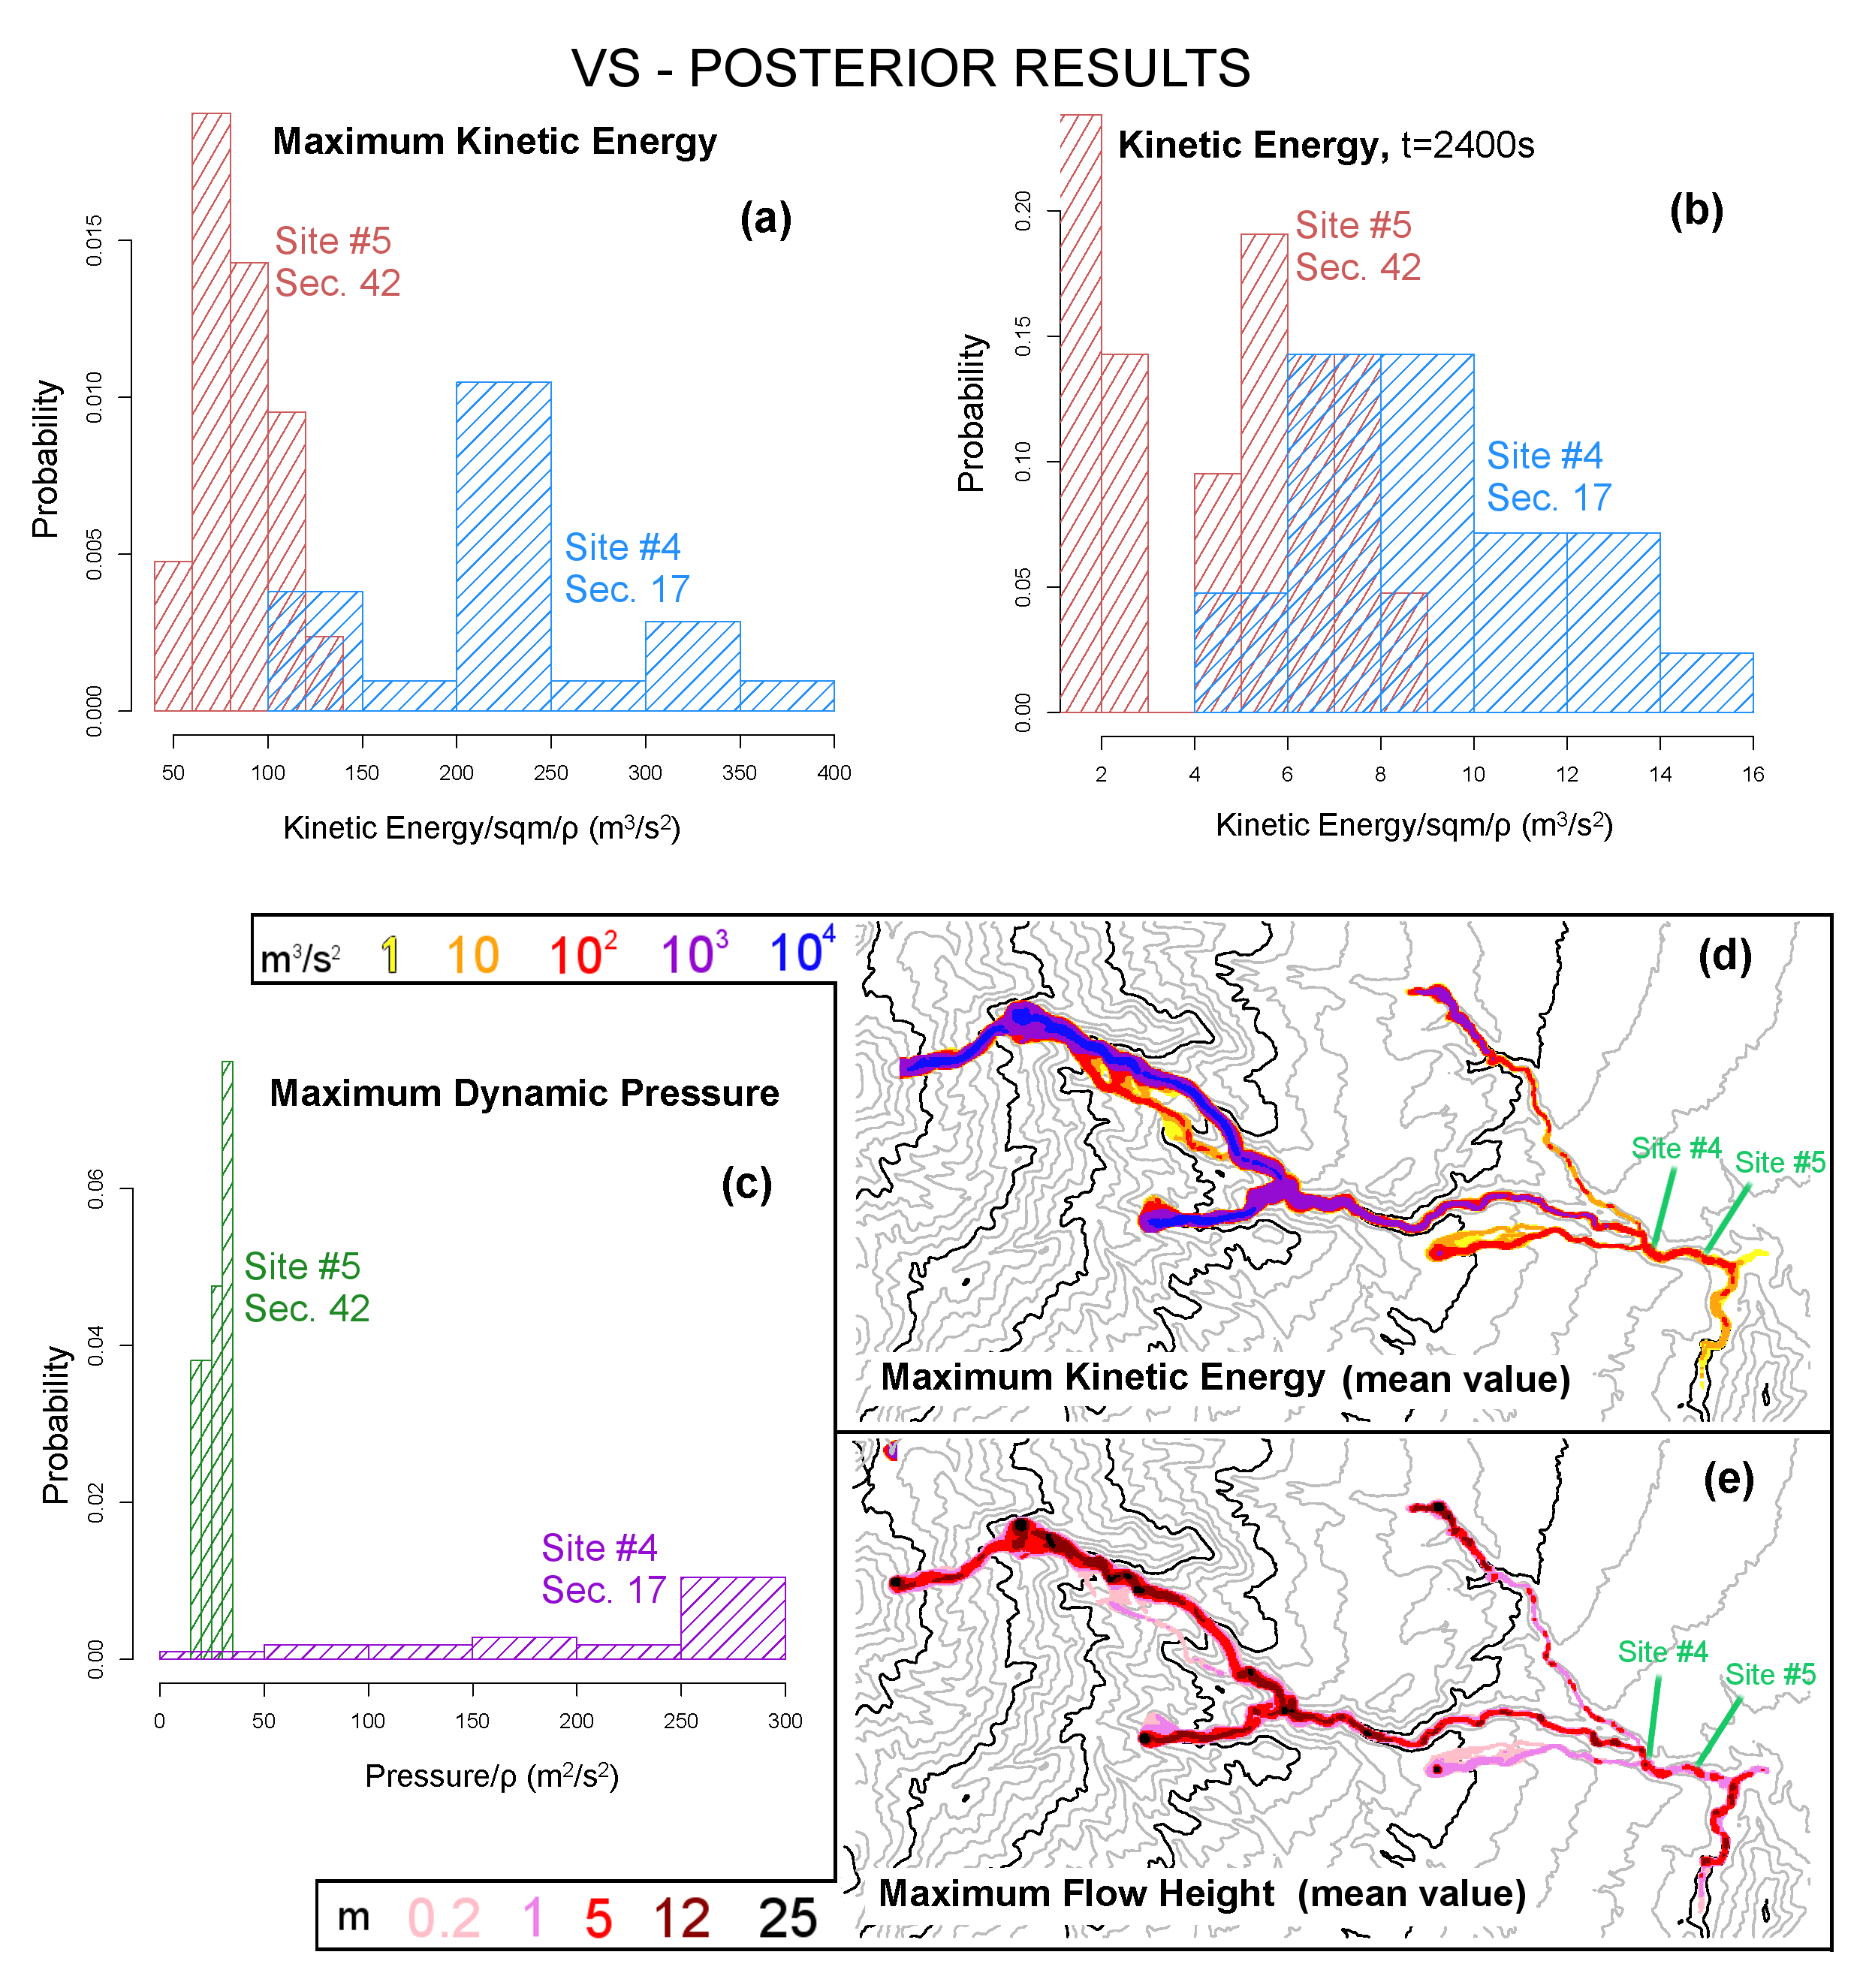
\includegraphics[width=1\textwidth]{Fig12.png}
\caption{Flow properties of VS model, over the input space $\tilde\Theta_2^{\textrm{VS}}$. Histograms of (a,b) local kinetic energy and (c) dynamic pressure in Sites \#4 and \#5, (a) at $t=2400$ s, (b,c) maximum value. Different sites are displayed with different colors. Mean values over $\tilde\Theta_2^{\textrm{VS}}$ of the maps of maximum (d) kinetic energy and (e) flow height as a function of time. Colors are related to their values. Elevation contours are included at intervals of 100 m (gray) and 500 m (black) \citep{NASA2014}. Sites \#4 and \#5 are displayed.}
\label{Fig12}
\end{figure}
In Figure \ref{Fig12a}, at Site \#4:
$$K\in[35,\ 75]\ m^3/s^2,\quad \kappa_f\in[3,\ 8]\ m^3/s^2,\quad Q\in[8,\ 13]\ m^2/s^2$$
and at Site \#5:
$$K\in[18,\ 34]\ m^3/s^2,\quad \kappa_f\in[1,\ 7]\ m^3/s^2,\quad Q\in[4,\ 7]\ m^2/s^2$$
Modal values are not well-constrained in this case.

\begin{figure}[H]
\centering
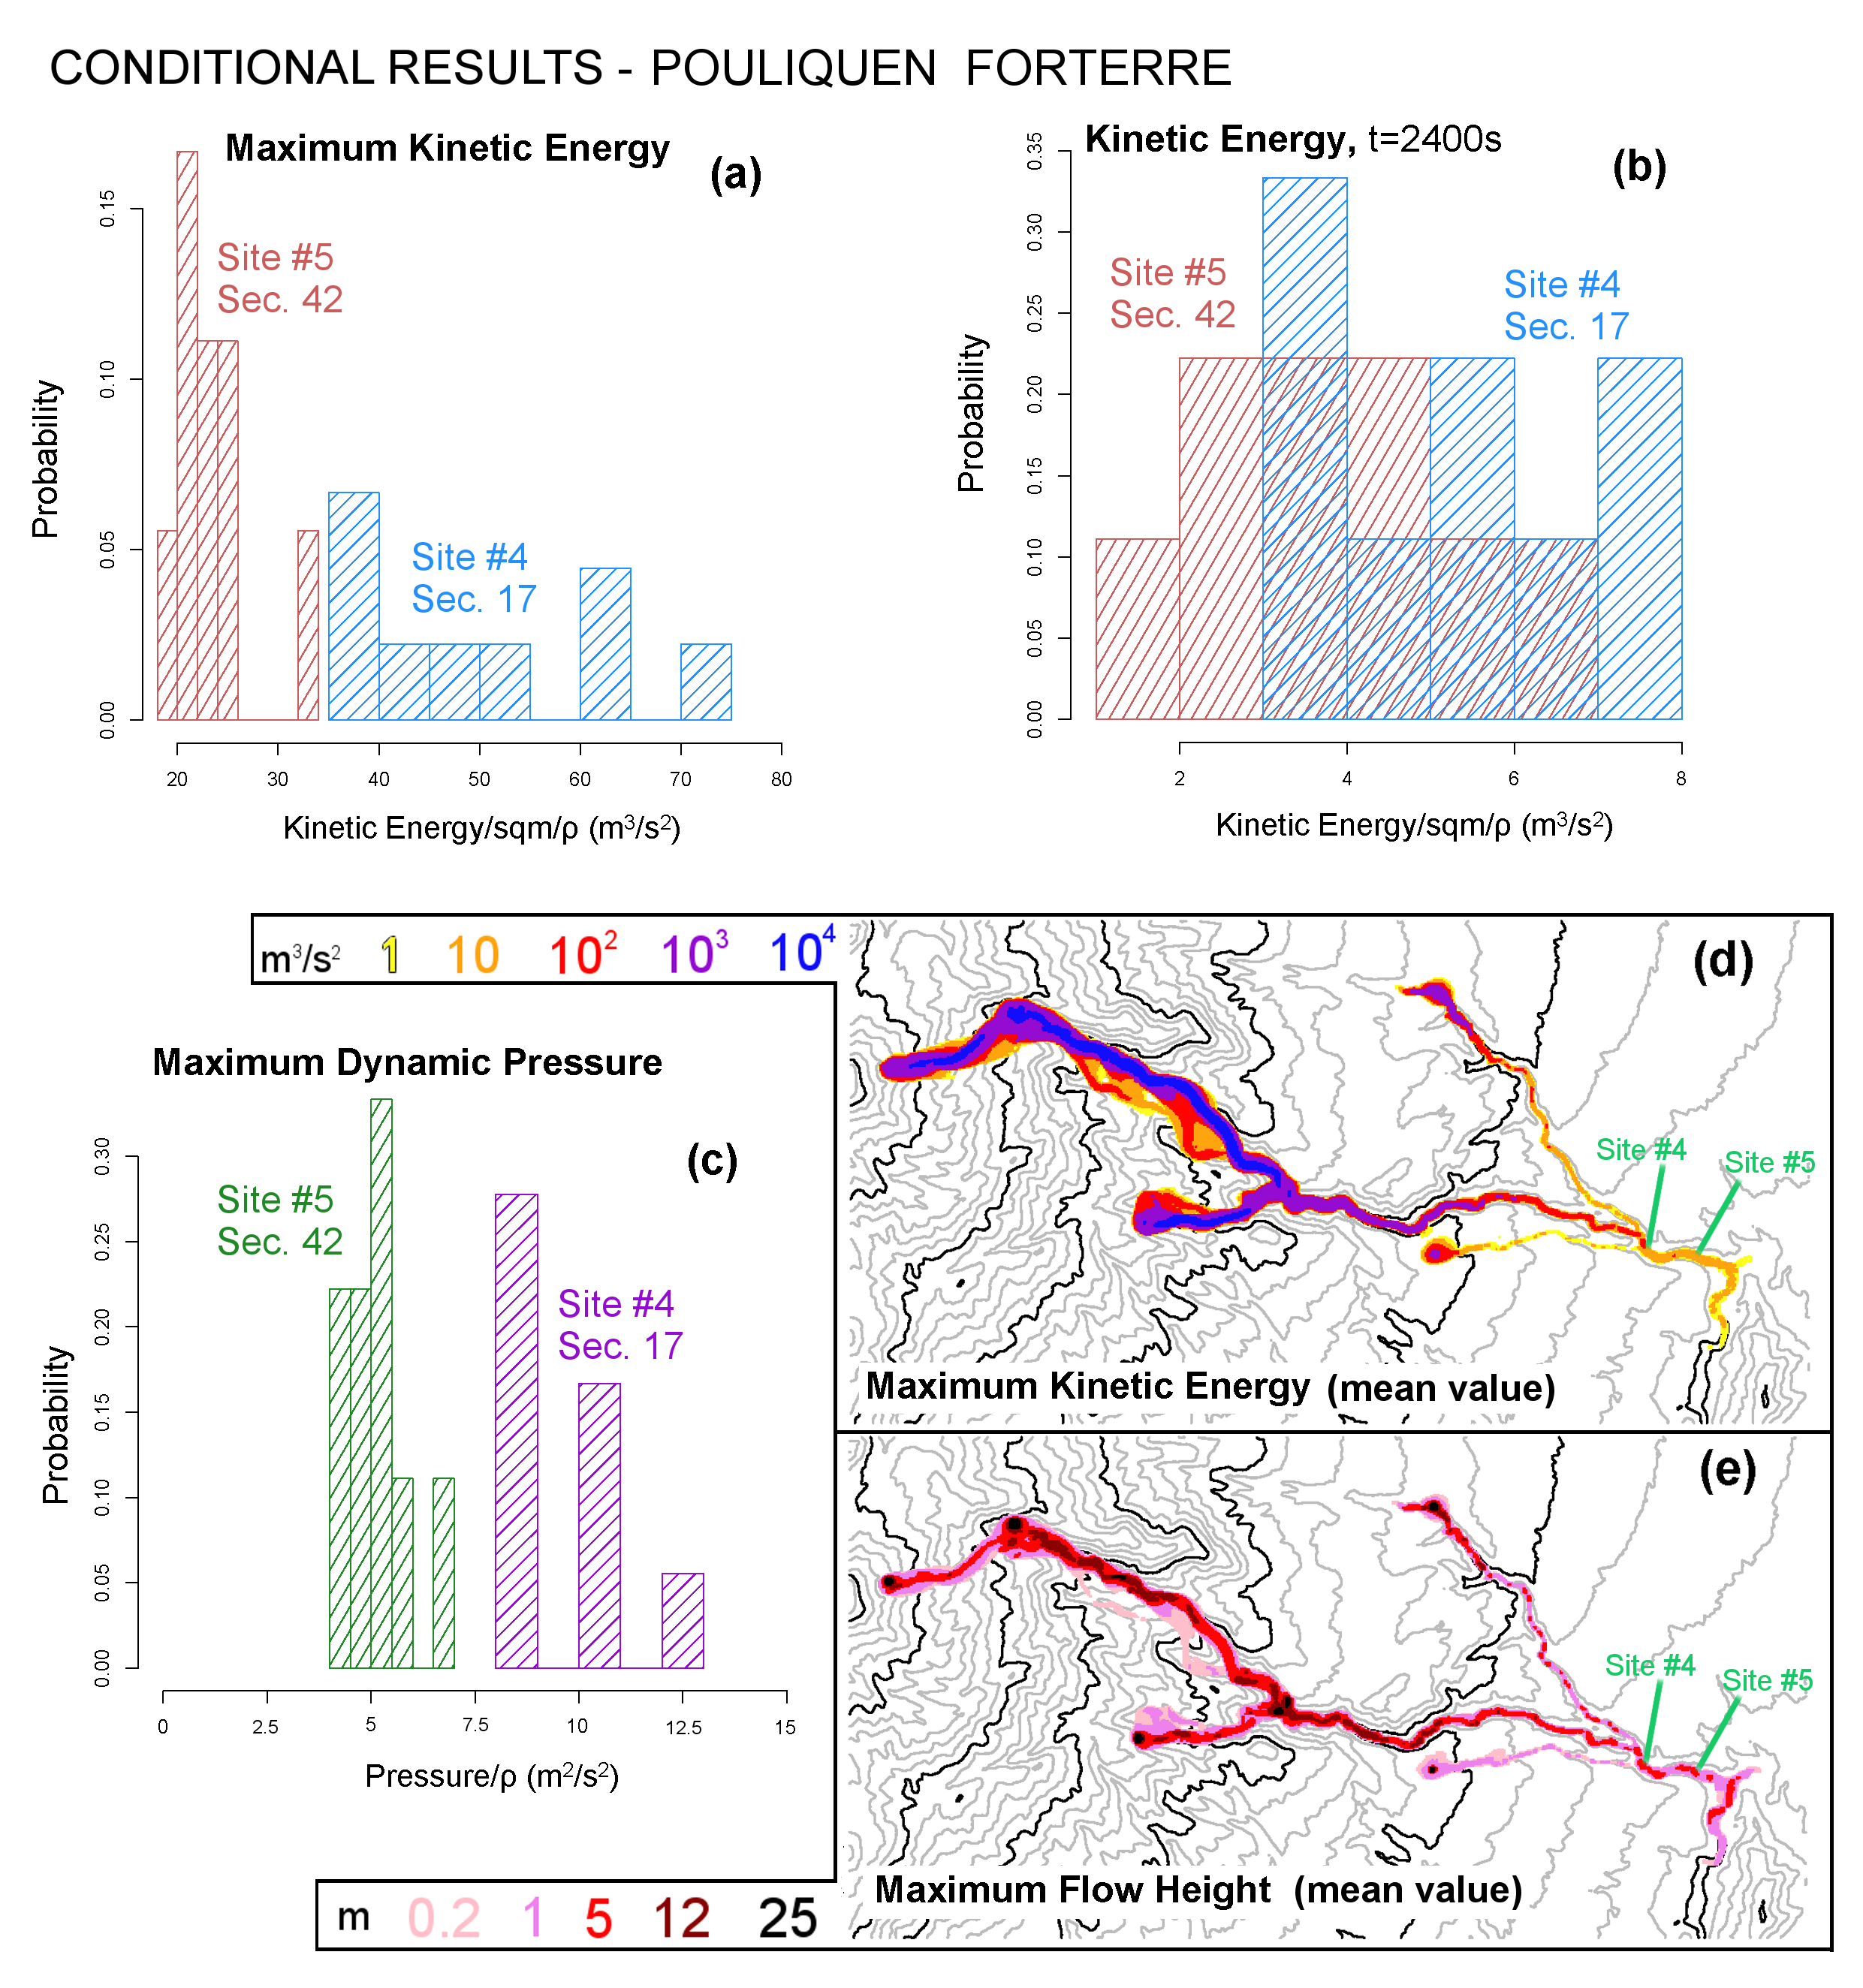
\includegraphics[width=1\textwidth]{Fig12_PF.png}
\caption{Flow properties of PF model, over the input space $\tilde\Theta_3^{\textrm{PF}}$. Histograms of (a,b) local kinetic energy and (c) dynamic pressure in Sites \#4 and \#5, (a) at $t=2400$ s, (b,c) maximum value. Different sites are displayed with different colors. Mean values over $\tilde\Theta_3^{\textrm{PF}}$ of the maps of maximum (d) kinetic energy and (e) flow height as a function of time. Colors are related to their values. Elevation contours are included at intervals of 100 m (gray) and 500 m (black) \citep{NASA2014}. Sites \#4 and \#5 are displayed.}
\label{Fig12a}
\end{figure}

In the spatial maps, PF shows slightly lower maximum flow height, and significantly lower energy than VS, especially in the distal part of the domain. The flow in the tributaries can reach the village, except for the smallest flows of Arroyo Pl\'atanos in PF, which however at $t_f$ are only tens of meters from the main branch. As in the unconditional maps, local maxima of flow height are located in the ravine, while the kinetic energy shows a more regular decrease.

We remark that the assumed $[4,\ 6]\ m/s$ constraint on the maximum flow speed has an immediate effect on the dynamic pressure estimates. Imposing it at Site \#5 as in the VS example, or Site \#4 as in the PF example, can radically changes the results, even if the deposit thickness at Site \#5 is still in $[1.4, 3.8]$ m.


%xx Need a paragraph or two here that discusses and summarizes what was learned about the Atenquique flow: what is the best estimated rheology?  What are the best estimated parameter values?  Does any rheology "work" or do all rheologies "work" in some sense?  What is the cut-off value for work/not work?  etc xx

\section{Conclusions}
In this study, we have introduced a new prediction-oriented method for the hazard assessment of volcaniclastic debris flows (lahars), based on multiple geophysical mass flow models. In particular, our approach has the advantage to decompose the original inverse problem into a hierarchy of simpler problems, and allows for the exploration of the impact of synthetic flows that are similar to those that occurred in the past, but different in plausible ways.

We applied our procedure to the case study of the 1955 Atenquique volcaniclastic debris flow. We adopted and compared three depth averaged models based on the Saint-Venant equations and widely used in hazard assessments. In summary:
\begin{itemize}
  \item We defined a \emph{specialized experimental design} after assuming: the existence of the numerical output, the realism of the underlying physics, robust numerical simulation, meaningful flow dynamics, and/or the capability to inundate a designated region. This produced a wide range of outputs which contain valuable information for hazard assessment.
\end{itemize}
Indeed, these outputs are not strictly reconstructing past flows and hence can provide hazard estimates under weaker constraints, potentially including extreme cases. Moreover, our designs were not trivial geometrically, due to the correlated effects of model inputs. This is a first step towards the development of a non-subjective and partially automated experimental design construction.
\begin{itemize}
  \item We statistically described the characteristics of the outputs and contributing variables by performing a Monte Carlo simulation over the specialized design. We mapped them globally and detailed them locally. This allowed us to calculate the likelihood of different model realizations given multiple pieces of information regarding the 1955 debris flow, providing useful information in either model selection or data inversion.
\end{itemize}
Our analysis concerned the mean values and also the uncertainty percentiles of the quantities of interest. Moreover, the probabilistic setting allowed us to implement the uncertainty affecting observed data. We also included information about contributing variables, which shed light over the different assumptions underlying the models.
\begin{itemize}
  \item We constructed partial solutions, conditioning the specialized experimental design to be consistent with three example subsets of observed data. We also described and intersected the corresponding inputs sets. We found model selection to be inherently linked to the inversion problem. That is, the partial inverse problems enabled us to select models, and the model choice nevertheless depended on the required properties and the spatial location.
\end{itemize}

%xx Need a conclusion here about the best estimated model of the Atenquique debris flow xx

The connection of inverse problems and model uncertainty thus represents a fundamental challenge in the future development of multi-model solvers dynamically selecting the model based on the performance against local data.

\section*{Acknowledgements}
We would like to acknowledge the support of NSF awards 1521855, 1621853, and 1339765. We would like to thank Byron Rupp for his fundamental work on the localization and volume constraints of the Atenquique debris flow \citep{Rupp2004}, and Ali Akhavan Safaei for the C++ and Python scripts to collect the local outputs and contributing variables on the grid elements \citep{Ali2018}.

\appendix
\section{Overview of the depth-averaged models}\label{A-1}
Many models based on different assumptions from those adopted in this study are available in literature, either more complex \citep{PitmanLe2005,Iverson2014} or more simple \citep{DadeHuppert1998}. We decided to focus on these three because of their historical relevance, and because they are all incorporated in our large scale mass flow simulation framework TITAN2D. We also remark that the poorly constrained data available for the past flow would make the application of a more complex model increasingly difficult.

\subsection{Mohr-Coulomb}\label{MCM}
Based on the long history of studies in soil mechanics \citep{Rankine1857,DruckerPage52}, the Mohr-Coulomb rheology (MC) was developed and used to represent the behavior of geophysical mass flows \citep{SavageHutter1989}. Shear and normal stress are assumed to obey Coulomb friction equation, both within the flow and at its boundaries. In other words,
\begin{equation}
\tau = \sigma \tan \phi,
\end{equation}
where $\tau$ and $\sigma$ are respectively the shear and normal stresses on failure surfaces, and $\phi$ is a friction angle. This relationship does not depend on the flow speed.

We can summarize the MC rheology assumptions as:
\begin{itemize}
\item \textit{Basal Friction} based on a constant friction angle.

\item \textit{Internal Friction} based on a constant friction angle.

\item \textit{Earth pressure coefficient} formula depends on the Mohr circle (implicitly depends on the friction angles).

\item Velocity based \textit{curvature effects} are included into the equations.
\end{itemize}

Under the assumption of symmetry of the stress tensor with respect to the \textit{z} axis, the earth pressure coefficient $k=k_{ap}$ can take on only one of three values $\{ 0, \pm 1\}$. The material yield criterion is represented by the two straight lines at angles $\pm \phi$ (the internal friction angle) relative to horizontal direction. Similarly, the normal and shear stress at the bed are represented by the line $\tau=-\sigma \tan(\delta)$ where $\delta$ is the bed friction angle.

\paragraph{MC equations} As a result, we can write down the source terms of the Eqs. (\ref{eq:D_A}):
\begin{eqnarray}\label{S_terms_MC}
S_x =& g_x h  - \frac{\bar{u}}{\| \underset{^\sim}{\bar{\textbf u}} \|} \left[h\left(g_z+\frac{\bar{u}^2}{r_x}\right)\tan(\phi_{bed})\right] - h k_{ap} \ {\rm sgn}\left(\frac{\partial \bar{u}}{\partial y}\right) \frac{\partial (g_z h)}{\partial y} \sin(\phi_{int}) \nonumber \\
 S_y =& g_y h  - \frac{\bar{v}}{\| \underset{^\sim}{\bar{\textbf u}} \|} \left[h\left(g_z +\frac{\bar{v}^2}{r_y}\right)\tan(\phi_{bed})\right] - h k_{ap} \ {\rm sgn}\left({\frac{\partial \bar{v}}{\partial x}}\right) \frac{\partial (g_z h)}{\partial x} \sin(\phi_{int})
\end{eqnarray}
Where, $\underset{^\sim}{\bar{\textbf u}} = (\bar{u} , \bar{v})$, is the depth-averaged velocity vector, $r_x$ and $r_y$ denote the radii of curvature
of the local basal surface. The inverse of the radii of curvature is usually approximated with the partial derivatives of the basal slope, e.g., $1/r_x = \partial \theta_x/\partial x$, where $\theta_x$ is the local bed slope.

\subsection{Pouliquen-Forterre}\label{PFM}
The scaling properties for granular flows down rough inclined planes led to the development of the Pouliquen-Forterre rheology (PF), assuming a variable frictional behavior as a function of Froude Number and flow depth \citep{Pouliquen1999, ForterrePouliquen2002, PouliquenForterre2002, ForterrePouliquen2003}.

PF rheology assumptions can be summarized as:
\begin{itemize}
\item \textit{Basal Friction} is based on an interpolation of two different friction angles, based on the flow regime and depth.

\item \textit{Internal Friction} is neglected.

\item \textit{Earth pressure coefficient} is equal to one.

\item Normal stress is modified by a \textit{pressure force} related to the flow thickness gradient.

\item Velocity based \textit{curvature effects} are included into the equations.
\end{itemize}

Two critical slope inclination angles are defined as functions of the flow thickness, namely $\phi_{start}(h)$ and $\phi_{stop}(h)$. The function $\phi_{stop}(h)$ gives the slope angle at which a steady uniform flow leaves a deposit of thickness $h$, while $\phi_{start}(h)$ is the angle at which a layer of thickness $h$ is mobilized. They define two different basal friction coefficients.
\begin{eqnarray}
\mu_{start}(h)=\tan(\phi_{start}(h))\\
\mu_{stop}(h)=\tan(\phi_{stop}(h))
\end{eqnarray}

An empirical friction law $\mu_{b}(\|\underset{^\sim}{\bar{\textbf{u}}} \| , h)$ is then defined in the whole range of velocity and thickness. The expression changes depending on two flow regimes, according to a parameter $\beta$ and the Froude number $Fr=\| \underset{^\sim}{\bar{\textbf{u}}} \| / \ \sqrt{h g_{z}}$.

\paragraph{Dynamic friction regime - $Fr \ge \beta$}
\begin{equation}\label{mu_beta1}
\mu(h, Fr)=\mu_{stop}(h \beta / Fr)
\end{equation}

\paragraph{Intermediate friction regime - $0 \le Fr < \beta$}
\begin{equation}\label{mu_beta2}
\mu(h, Fr)=\left(\frac{Fr}{\beta}\right)^\gamma [\mu_{stop}(h)-\mu_{start}(h)] + \mu_{start}(h),
\end{equation}
where $\gamma$ is the power of extrapolation, assumed equal to $10^{-3}$ in the sequel \citep{PouliquenForterre2002}.

The functions $\mu_{stop}$ and $\mu_{start}$ are defined by:
\begin{equation}\label{mu-stop}
\mu_{stop}(h)=\tan\phi_{1} + \frac{\tan\phi_{2}-\tan\phi_{1}}{1+h/\it \mathcal{L}}
\end{equation}
and
\begin{equation}\label{mu-start}
\mu_{start}(h)=\tan\phi_{3} + \frac{\tan\phi_{2}-\tan\phi_{1}}{1+h/\it \mathcal{L}}
\end{equation}
The critical angles $\phi_{1}$, $\phi_{2}$ and $\phi_{3}$ and the parameters $\mathcal{L}, \beta$ are the parameters of the model.

In particular, $\mathcal{L}$ is the characteristic depth of the flow over which a transition between the angles $\phi_{1}$ to $\phi_{2}$ occurs, in the $\mu_{stop}$ formula. In practice, if $h\ll \mathcal L$, then $\mu_{stop}(h)\approx \tan\phi_{2}$, and if $h\gg \mathcal L$, then $\mu_{stop}(h)\approx\tan\phi_{1}$.

\paragraph{PF equations} The depth-averaged Eqs. (\ref{eq:D_A}) source terms thus take the following form:
\begin{eqnarray}\label{eq:S_terms_PF}
S_{x} &=&  g_{x} h -  \frac{\bar{u}}{\| \underset{^\sim}{\bar{\textbf{u}}} \|}\left[h \left(g_z+\frac{\bar{u}^2}{r_x}\right) \ \mu_{b}(\|\underset{^\sim}{\bar{\textbf{u}}} \| , h)\right] \ + g_{z}h\frac{\partial h}{\partial x} \nonumber \\
S_{y} &=&  g_{y} h - \frac{\bar{v}}{\| \underset{^\sim}{\bar{\textbf{u}}} \|}\left[h \left(g_z +\frac{\bar{v}^2}{r_y}\right) \ \mu_{b}(\|\underset{^\sim}{\bar{\textbf{u}}} \| , h)\right] \ + g_{z}h\frac{\partial h}{\partial y}
\end{eqnarray}

\subsection{Voellmy-Salm}\label{VSM}
The theoretical analysis of dense snow avalanches led to the VS rheology (VS) \citep{Voellmy1955, Salm1990, Salm1993, Bartelt1999}. Dense snow or debris avalanches consist of mobilized, rapidly flowing ice-snow mixed to debris-rock granules \citep{BarteltMcArdell2009}. The VS rheology assumes a velocity dependent resisting term in addition to the traditional basal friction, ideally capable of including an approximation of the turbulence-generated dissipation. Many experimental and theoretical studies were developed in this framework \citep{Gruber2007, Kern2009, Christen2010, Fischer2012}. The following relation between shear and normal stresses holds:
\begin{equation}
\tau = \mu \sigma + \frac{\rho \| \underline{\textbf g} \|}{\xi} \| \underset{^\sim}{\bar{\textbf u}} \|^2,
\end{equation}
where, $\sigma$ denotes the normal stress at the bottom of the fluid layer and $\underline{\textbf g} = (g_{x} , g_{y} , g_{z})$ represents the gravity vector. The two parameters of the model are the bed friction coefficient $\mu$ and the velocity dependent friction coefficient $\xi$.

We can summarize VS rheology assumptions as:
\begin{itemize}
\item \textit{Basal Friction} is based on a constant coefficient, similarly to the MC rheology.

\item \textit{Internal Friction} is neglected.

\item \textit{Earth pressure coefficient} is equal to one.

\item Additional \textit{turbulent friction} is based on the local velocity by a quadratic expression.

\item Velocity based \textit{curvature effects} are included into the equations, following an alternative formulation.
\end{itemize}

The effect of the topographic local curvatures is addressed with terms containing the local radii of curvature $r_x$ and $r_y$. In this case the expression is based on the speed instead of the scalar components of velocity \citep{PudasainiHutter2003,Fischer2012}.

\paragraph{VS equations} Therefore, the final source terms take the following form:
\begin{eqnarray}
\label{eq:S_terms_VS}
S_{x} &=&  g_{x} h - \frac{\bar{u}}{\| \underset{^\sim}{\bar{\textbf u}}\|} \ \left[ h \left(g_{z} + \frac{\| \underset{^\sim}{\bar{\textbf u}} \|^2}{r_{x}} \right)\mu+ \frac{\| \underset{^\sim}{\textbf g} \|}{\xi}\| \underset{^\sim}{\bar{\textbf u}} \|^2\right], \nonumber \\
S_{y} &=& g_{y} h - \frac{\bar{v}}{\| \underset{^\sim}{\bar{\textbf u}}\|} \ \left[ h \left(g_{z} + \frac{\| \underset{^\sim}{\bar{\textbf u}} \|^2}{r_{y}} \right)\mu+ \frac{\| \underset{^\sim}{\textbf g} \|}{\xi}\| \underset{^\sim}{\bar{\textbf u}} \|^2\right].
\end{eqnarray}

\section{Contributing variables}\label{A-2}
Let $\left[F_n(\underline{\textbf x},t)\right]_{n=1,\dots, N}$ be an array of force terms, where $\underline{\textbf x}\in \mathbf R^d$ is a spatial location, and $t\in T$ is a time instant. The degree of contribution of those force terms to the flow dynamics can be significantly variable in space and time, and we define the \emph{dominance factors} $[p_n(\underline{\textbf x},t)]_{n=1,\dots, N}$, i.e., the probability of each $F_n(\underline{\textbf x},t)$ to be the dominant force. Those probabilities provide insight into the dominance of a particular source or dissipation term on the model dynamics. We remark that we focus on the modulus of the forces and hence we cope with scalar terms. It is also important to remark that all the forces depend on the input variables, and they can be thus considered as random variables. Furthermore, these definitions are general and could be applied to any set of contributing variables, and not only to the force terms. More details about this can be found in \cite{Patra2018}.

\begin{definition}[Dominance factors]
Let $(F_i)_{i\in I}$ be random variables on $(\Omega, \mathcal F, P_M)$. Then, $\forall i$, the dominant variable is defined as:
$$\Phi:=\max_i |F_i|.$$
In particular, for each $j \in I$, the dominance factors are defined as:
$$p_j:=P_M\left\{\Phi=|F_j|\right\}.$$
\end{definition}

Moreover, we define the \emph{random contributions}, an additional tool that we use to compare the different force terms, following a less restrictive approach than the dominance factors. They are obtained dividing the force terms by the dominant force $\Phi$, and hence belong to $[0,1]$.

\begin{definition}[Expected contributions]
Let $(F_i)_{i\in I}$ be random variables on $(\Omega, \mathcal F, P_M)$. Then, $\forall i$, the random contribution is defined as:
$$C_i:=\left\{
\begin{array}{ll}
      \frac{F_i}{\Phi}, & \textrm{if }\Phi\neq 0; \\
      0, & \hbox{otherwise.}
    \end{array}
  \right.$$
where $\Phi$ is the dominant variable. Thus, $\forall i$, the expected contributions are defined by $E\left[C_i\right]$.
\end{definition}

In particular, for a particular location $x$, time $t$, and parameter sample $\omega$, we have $C_n(\underline{\textbf x},t,\omega)=0$ if there is no flow or all the forces are null. The expectation of $C_n$ is reduced by the chance of $F_n$ being small compared to the other terms, or by the chance of having no flow in $(\underline{\textbf x},t)$.

\bibliographystyle{apalike}
\bibliography{mybibfileMX}
\end{document} 